% =====================================================================================
% main.tex -- What a target-domain training signal buys a sim-to-real lens finder on Euclid Q1,
% from a balanced to a 1:10 target (paper v6; earlier titles from rewrites v1 and v5).
% =====================================================================================
%
% Full draft: prose in sections/, generated tables and figures, appendices partly written.
%
% Build:
%     pdflatex main && bibtex main && pdflatex main && pdflatex main
%
% Everything under tables/ and figures/ is GENERATED. Never edit those files; rebuild
% them with
%     python paper/scripts/make_all.py
% and see paper/README.md for what each script reads.
%
% Class choice: a stock single-column `article`. The OJAp style file swaps in later; the
% tables are emitted as ordinary floats at \footnotesize so they fit this text block,
% and paper/scripts/_common.py:write_table is the single place that changes if a
% two-column style is adopted.
% =====================================================================================
\documentclass[11pt,a4paper]{article}

\usepackage[T1]{fontenc}
\usepackage[utf8]{inputenc}
\usepackage{lmodern}
\usepackage[margin=1in]{geometry}

\usepackage{amsmath}
\usepackage{amssymb}
\usepackage{graphicx}
\usepackage{booktabs}
\usepackage{xcolor}
\usepackage{array}
% placeins [section]: a \FloatBarrier at every \section, so no float drifts past it.
\usepackage[section]{placeins}
\usepackage[numbers,sort&compress]{natbib}
\usepackage[colorlinks=true,allcolors=blue]{hyperref}

% Float placement. The generated tables are emitted as [tbp] floats
% (paper/scripts/_common.py:write_table); these limits let a tall table share a page with
% text instead of being deferred to the end of the document.
\renewcommand{\topfraction}{0.9}
\renewcommand{\bottomfraction}{0.8}
\renewcommand{\textfraction}{0.07}
\renewcommand{\floatpagefraction}{0.7}
\setcounter{topnumber}{3}
\setcounter{totalnumber}{4}

% Ragged-right paragraph cells in the generated tables: >{\TRAG}p{<width>}. The name is
% upper-case on purpose -- check_latex.py counts the lower-case l/c/r/p letters of a column
% spec, so a macro spelled in capitals adds no phantom column.
\newcommand{\TRAG}{\raggedright\arraybackslash}

% Lines carrying several inline intervals or a long \texttt identifier cannot be broken
% inside them; a little emergency stretch lets TeX set such a paragraph slightly looser
% instead of pushing a box into the margin. Paragraphs that set well are unaffected.
\setlength{\emergencystretch}{2.5em}

% Every generated table puts its \caption above the tabular, and article's \belowcaptionskip
% is 0pt, so a caption's last line can touch the table's top rule. One fixed gap, tables only
% (figures keep their captions below with the class defaults); a kernel hook, no package.
% 4pt is the largest gap that keeps the paper at 49 pages (5pt and 6pt give 50; PROJECTv7 7.62).
\AddToHook{env/table/begin}{\setlength{\belowcaptionskip}{4pt}}

\graphicspath{{figures/}}

% \todo marks unfinished content. make_archive.py refuses to build paper.zip while any
% remains (see paper/README.md).
\newcommand{\todo}[1]{\textcolor{red}{\textbf{[TODO: #1]}}}

% Generated number macros (paper/scripts/make_m_sim_zl.py); prose quotes these, never
% a retyped value.
% GENERATED FILE -- do not edit by hand.
% Rebuild:  python make_all.py (generator: make_m_sim_zl.py)
% Macros: deflector-redshift summary of the 30,000 simulated lenses.
% Source: paper/data/sim_zl.json (written by this script from the shards).
\newcommand{\simZlMedian}{0.65}
\newcommand{\simZlPTen}{0.48}
\newcommand{\simZlPNinety}{0.76}

% GENERATED FILE -- do not edit by hand.
% Rebuild:  python make_all.py (generator: make_a4_augprec.py)
% Macros for Section 4 and Appendix A4, from paper/data/lever1_aug_precision_D1.json.
\newcommand{\augprecTrainable}{1{,}921}
\newcommand{\augprecTotal}{$-0.0816$}
\newcommand{\augprecTotalCI}{$[-0.1429, -0.0102]$}
\newcommand{\augprecTotalLenses}{8}
\newcommand{\augprecAug}{$-0.0612$}
\newcommand{\augprecAugCI}{$[-0.1327, +0.0000]$}
\newcommand{\augprecAugLenses}{6}
\newcommand{\augprecPrec}{$-0.0204$}
\newcommand{\augprecPrecCI}{$[-0.0510, +0.0204]$}
\newcommand{\augprecPrecLenses}{2}
\newcommand{\augprecCellA}{$0.2347$}
\newcommand{\augprecCellC}{$0.1531$}
\newcommand{\augprecOnePos}{$0.0102$}
\newcommand{\augprecBaselineFoldZero}{$0.2449$}
\newcommand{\augprecCellCKaggle}{$0.1735$}
\newcommand{\augprecVenueDiff}{$0.0204$}
\newcommand{\augprecVenueLenses}{2}
\newcommand{\augprecVenueCI}{$[-0.0204, +0.0510]$}

% GENERATED FILE -- do not edit by hand.
% Rebuild:  python paper/scripts/make_a5_restart.py
% Macros for Section 8 and Appendix A5 (see paper/scripts/make_a5_restart.py for sources).
\newcommand{\restartKeys}{\texttt{head\_type}, \texttt{head}, \texttt{standardizer}, \texttt{cfg}}
\newcommand{\restartMuZeroSteps}{800}
\newcommand{\restartScheduleSteps}{8{,}000}
\newcommand{\restartControlSteps}{2{,}000}
\newcommand{\restartStart}{$0.3878$}
\newcommand{\restartTrough}{$0.2347$}
\newcommand{\restartTroughStep}{500}
\newcommand{\restartEnd}{$0.3367$}
\newcommand{\restartMaxDrift}{$0.1531$}
\newcommand{\restartMaxDriftPos}{15}
\newcommand{\restartRecovery}{$0.1020$}
\newcommand{\restartOnePos}{$0.0102$}
\newcommand{\restartFixedMaxDrift}{$0.0408$}
\newcommand{\restartFixedMaxDriftPos}{4}
\newcommand{\restartFixedMean}{$0.3686$}
\newcommand{\restartFixedSD}{$0.0107$}
\newcommand{\restartFixedN}{16}
\newcommand{\restartTailMean}{$0.3696$}
\newcommand{\restartTailSD}{$0.0105$}
\newcommand{\restartTailN}{9}
\newcommand{\restartSatPasses}{40}
\newcommand{\restartPool}{782}
\newcommand{\restartSatBatches}{160}
\newcommand{\restartEmaIters}{5{,}000}
\newcommand{\restartMomentum}{0.999}
\newcommand{\restartTauDirect}{$0.9586$}
\newcommand{\restartTauAgree}{$5.1 \times 10^{-6}$}
\newcommand{\restartPbarAgree}{$9.1 \times 10^{-5}$}
\newcommand{\restartSatTol}{$5 \times 10^{-3}$}
\newcommand{\restartMuOffset}{8{,}000}
\newcommand{\restartAdamSteps}{200}
\newcommand{\restartAdamDebiased}{+2.22\%}
\newcommand{\restartAdamProbeEnd}{500}

% GENERATED FILE -- do not edit by hand.
% Rebuild:  python make_all.py (generator: make_orderings_v3.py)
% The contrast count (rewrite v3), len(_common.CONTRAST_ROWS); replaces M_orderings.tex in main.tex.
\newcommand{\contrastCount}{13}

% GENERATED FILE -- do not edit by hand.
% Rebuild:  python make_all.py (generator: make_m_venue.py)
% Macros for Section 4's venue paragraph; sources in paper/scripts/make_m_venue.py.
\newcommand{\venueTrainPrecision}{fp16}
\newcommand{\venueEvalPrecision}{fp32}
\newcommand{\venueGpu}{Tesla~T4}
\newcommand{\venueGpuArms}{CORAL, DANN, BNM and $\lambda{=}0$}
\newcommand{\venueCoralCheckpoints}{9}
\newcommand{\venueCoralMaxAuroc}{$2.1 \times 10^{-5}$}

% GENERATED FILE -- do not edit by hand.
% Rebuild:  python paper/scripts/make_m_batch.py
% Macros for Section 4's batch-composition sentence; sources in paper/scripts/make_m_batch.py.
\newcommand{\batchSourceRows}{256}
\newcommand{\batchTargetRows}{256}
\newcommand{\batchSourcePositives}{128}

% GENERATED FILE -- do not edit by hand.
% Rebuild:  python make_all.py (generator: make_m_sim_source.py)
% Macros for Section 3's source description, parsed from scripts/generate_arc_on_real.py; sources in paper/scripts/make_m_sim_source.py.
\newcommand{\simSourceSample}{23.5}
\newcommand{\simSourceGalType}{parametric}
\newcommand{\simSourceHlrMin}{0.15}
\newcommand{\simSourceHlrMax}{1.5}
\newcommand{\simArcSnrMin}{5}
\newcommand{\simArcSnrMax}{30}

% GENERATED FILE -- do not edit by hand.
% Rebuild:  python make_all.py (generator: make_m_zoobot2.py)
% Macros for Section 4's pretraining sentence; transcribed literature values in paper/data/zoobot2_pretraining.json.
\newcommand{\zoobotPretrainImages}{842\,000}
\newcommand{\zoobotPretrainCampaigns}{6}

% GENERATED FILE -- do not edit by hand.
% Rebuild:  python make_all.py (generator: make_a2_hashes.py)
% Macros for Appendix A2's DANN pre-fold paragraph and the lambda=0 Kaggle date, asserted from the evidence files by paper/scripts/make_a2_hashes.py.
\newcommand{\dannPrefoldEntry}{10}
\newcommand{\dannPrefoldSha}{51351308}
\newcommand{\dannArcEntry}{5}
\newcommand{\dannPrefoldIdenticalKeys}{35}
\newcommand{\dannPrefoldAddedKeys}{4}
\newcommand{\lambdaKaggleDate}{6 September 2026}

% GENERATED FILE -- do not edit by hand.
% Rebuild:  python make_all.py (generator: make_a7_prereg_pool.py)
% Macros: the test pool (Sections 3 and 9).
% Test-pool macros for Sections 3 and 9, from audit/decontam/rule.json via
% scripts/exact_ids.contaminant_sets and the stored scores.
\newcommand{\DOneRemoved}{265}
\newcommand{\DOneLensNeg}{28}
\newcommand{\DOneDeflNeg}{237}
\newcommand{\DTwoPositives}{20}
\newcommand{\DeflOtherNeg}{320}
\newcommand{\DeflAllNeg}{557}
\newcommand{\DTwoMaxShift}{0.0100}
\newcommand{\DTwoMaxShiftArm}{Baseline A}
\newcommand{\TestNegDrawn}{26\,399}
\newcommand{\TestNegDOne}{26\,134}

% GENERATED FILE -- do not edit by hand.
% Rebuild:  python make_all.py (generator: make_m_prose.py)
% Macros for the result numbers quoted in the prose, test pool D1.
% Each prints as the typed number did: same decimals, same explicit sign.
% pre-registered pool (fold 0)
\newcommand{\baseFoldZeroPrereg}{0.1939}
% fold-0 window
\newcommand{\wzEightMultMinTwo}{0.96}
\newcommand{\wzEightMultMaxTwo}{1.95}
% Figure 6 curves (D8)
\newcommand{\dEightFmAbovePct}{77}
% deflector sample (deflector_cutouts_clean.npz)
\newcommand{\DeflMassFloor}{10.7}
\newcommand{\DeflZmin}{0.10}
\newcommand{\DeflZmax}{0.79}
\newcommand{\DeflUnphysMass}{12.5}
\newcommand{\DeflUnphysMag}{-26}
\newcommand{\DeflUnphysN}{19}
% deflectors drawn into the shards
\newcommand{\DeflUnphysDrawn}{17}
\newcommand{\DeflUnphysLenses}{132}
% grade-X list vs catalogue v0.0.3
\newcommand{\GradeXnowC}{8}
% splits.json source_train.neg_mlfp
\newcommand{\GradeXUsed}{4455}
% data/splits/dilute10_pool.json reference set c (dilute10 part 1)
\newcommand{\GradeXAll}{4940}
% scripts/01_query_catalog.py (MER query)
\newcommand{\FluxMin}{2.3}
\newcommand{\FluxMax}{229}
\newcommand{\MagFaint}{23.0}
\newcommand{\MagBright}{18.0}
% test negatives on pool D1, PSF magnitude > 22.5
\newcommand{\FracFaintTest}{43}

% Rewrite v1: the review-round numbers (paper/scripts/make_review_macros.py) and the
% main-text display variants at two decimals (paper/scripts/make_m_display.py).
% GENERATED FILE -- do not edit by hand.
% Rebuild:  python make_all.py (generator: make_review_macros.py)
% Macros for the review-round numbers (rewrite v1). Sources:
% audit/review_r1/out, audit/review_r1b/out (input hashes re-checked), PROJECTv7.md, run files.
% audit/review_r1/out/F4_fold_overlap.json
\newcommand{\rvSharedTargetMin}{293}
\newcommand{\rvSharedTargetMax}{294}
\newcommand{\rvTargetLensPool}{391}
\newcommand{\rvTargetOverlapPct}{75}
% audit/review_r1/out/F5_host_properties.json
\newcommand{\rvHostAurocMin}{0.46}
\newcommand{\rvHostAurocMax}{0.58}
\newcommand{\rvBareDeflN}{2881}
\newcommand{\rvSourceNegN}{24\,000}
\newcommand{\rvSourcePosN}{24\,000}
% audit/review_r1/out/F6_d2_lenses.json
\newcommand{\rvDTwoTrainNeg}{14}
\newcommand{\rvDTwoValNeg}{6}
\newcommand{\rvDTwoRandom}{19}
% audit/review_r1/out/F7_lenses_in_test_pool.json
\newcommand{\rvOwnPosMin}{4}
\newcommand{\rvOwnPosMax}{8}
\newcommand{\rvFsevenDaMin}{13}
\newcommand{\rvFsevenDaMax}{18}
\newcommand{\rvFsevenRefMin}{7}
\newcommand{\rvFsevenRefMax}{9}
\newcommand{\rvAboveThrN}{26}
% audit/decontam/rule.json
\newcommand{\rvRuleSha}{b83fa019}
% audit/review_r1/out/A1_resolution.json
\newcommand{\rvNoiseMin}{0.034}
\newcommand{\rvNoiseMax}{0.053}
\newcommand{\rvScale}{0.05}
\newcommand{\rvGapThreeMin}{0.005}
\newcommand{\rvGapThreeMax}{0.033}
\newcommand{\rvGapBnmMin}{0.09}
\newcommand{\rvGapBnmMax}{0.13}
\newcommand{\rvSigmaMin}{0.04}
\newcommand{\rvSigmaMax}{0.09}
\newcommand{\rvLagMin}{-0.09}
\newcommand{\rvLagMax}{+0.14}
% audit/review_r1/out/A2_top_negatives.json
\newcommand{\rvTopNegN}{191}
% audit/review_r1/out/A2_crossmatch.json
\newcommand{\rvTopNegC}{22}
% audit/review_r1/out/A3_recall_by_grade.json
\newcommand{\rvGradeRatioMin}{1.9}
\newcommand{\rvGradeRatioMax}{3.2}
% audit/review_r1/out/A2_magnitude_bias.json
\newcommand{\rvAboveFaintPct}{34}
\newcommand{\rvPoolFaintPct}{43}
% audit/review_r1/out/A3_recall_by_property.json
\newcommand{\rvThetaN}{245}
\newcommand{\rvConfTestN}{391}
% audit/review_r1/out/A3_galleries.json
\newcommand{\rvMissedAllN}{136}
\newcommand{\rvMissedAllB}{99}
% runs/{dann_main,baseline_unfrozen,bnm_r6_folds}/*/run.json (dann_d_holdout_n / target_holdout_n), all 12 folds; audit/review_r1b/out/L1_target_labels.json
\newcommand{\rvHoldoutN}{78}
% audit/review_r1b/out/L2_bright_pool.json
\newcommand{\rvBrightN}{14\,950}
\newcommand{\rvBnmBrightRatio}{0.55}
\newcommand{\rvBnmDOneRatio}{0.71}
% runs/bnm_r6_prereg.json
\newcommand{\rvGradShiftPct}{27.6}
% PROJECTv7.md:494 (no-DA head AUROC)
\newcommand{\rvEarlyNoDa}{0.61}
% PROJECTv7.md:4143 (plain DANN head AUROC)
\newcommand{\rvEarlyDann}{0.37}
% PROJECTv7.md:494 (IW-CDAN head AUROC)
\newcommand{\rvEarlyIw}{0.33}
% PROJECTv7.md:3178-3181 (frozen linear probe)
\newcommand{\rvEarlyProbe}{0.90}

% GENERATED FILE -- do not edit by hand.
% Rebuild:  python make_all.py (generator: make_m_display.py)
% Main-text display variants (two decimals, whole per cent), computed from the same calls as the four-decimal tables.
% Table 2 (_common.fold_mean, D1)
\newcommand{\dFmBaseline}{0.18}
\newcommand{\dSdBaseline}{0.03}
\newcommand{\dFmLambda}{0.18}
\newcommand{\dSdLambda}{0.03}
\newcommand{\dFmBnm}{0.40}
\newcommand{\dSdBnm}{0.04}
\newcommand{\dFmFreeMatch}{0.52}
\newcommand{\dSdFreeMatch}{0.07}
\newcommand{\dFmDann}{0.50}
\newcommand{\dSdDann}{0.17}
\newcommand{\dFmDannSens}{0.55}
\newcommand{\dSdDannSens}{0.11}
\newcommand{\dFmCoral}{0.52}
\newcommand{\dSdCoral}{0.08}
\newcommand{\dHeadMin}{0.40}
\newcommand{\dHeadMax}{0.52}
% Table 3 (_common.contrast, D1) row 0
\newcommand{\dCtLamBase}{0.00}
\newcommand{\dCtLamBaseLo}{-0.09}
\newcommand{\dCtLamBaseHi}{+0.09}
\newcommand{\dCtLamBaseAbs}{0.00}
\newcommand{\dCtLamBaseAbsLo}{0.09}
\newcommand{\dCtLamBaseAbsHi}{0.09}
% Table 3 (_common.contrast, D1) row 1
\newcommand{\dCtDannLam}{+0.31}
\newcommand{\dCtDannLamLo}{+0.06}
\newcommand{\dCtDannLamHi}{+0.57}
\newcommand{\dCtDannLamAbs}{0.31}
\newcommand{\dCtDannLamAbsLo}{0.06}
\newcommand{\dCtDannLamAbsHi}{0.57}
% Table 3 (_common.contrast, D1) row 2
\newcommand{\dCtCoralLamM}{+0.31}
\newcommand{\dCtCoralLamMLo}{+0.18}
\newcommand{\dCtCoralLamMHi}{+0.43}
\newcommand{\dCtCoralLamMAbs}{0.31}
\newcommand{\dCtCoralLamMAbsLo}{0.18}
\newcommand{\dCtCoralLamMAbsHi}{0.43}
% Table 3 (_common.contrast, D1) row 3
\newcommand{\dCtFmLamM}{+0.32}
\newcommand{\dCtFmLamMLo}{+0.20}
\newcommand{\dCtFmLamMHi}{+0.45}
\newcommand{\dCtFmLamMAbs}{0.32}
\newcommand{\dCtFmLamMAbsLo}{0.20}
\newcommand{\dCtFmLamMAbsHi}{0.45}
% Table 3 (_common.contrast, D1) row 4
\newcommand{\dCtBnmLam}{+0.22}
\newcommand{\dCtBnmLamLo}{+0.14}
\newcommand{\dCtBnmLamHi}{+0.30}
\newcommand{\dCtBnmLamAbs}{0.22}
\newcommand{\dCtBnmLamAbsLo}{0.14}
\newcommand{\dCtBnmLamAbsHi}{0.30}
% Table 3 (_common.contrast, D1) row 5
\newcommand{\dCtCoralLamP}{+0.34}
\newcommand{\dCtCoralLamPLo}{+0.19}
\newcommand{\dCtCoralLamPHi}{+0.49}
\newcommand{\dCtCoralLamPAbs}{0.34}
\newcommand{\dCtCoralLamPAbsLo}{0.19}
\newcommand{\dCtCoralLamPAbsHi}{0.49}
% Table 3 (_common.contrast, D1) row 6
\newcommand{\dCtFmLamP}{+0.33}
\newcommand{\dCtFmLamPLo}{+0.23}
\newcommand{\dCtFmLamPHi}{+0.44}
\newcommand{\dCtFmLamPAbs}{0.33}
\newcommand{\dCtFmLamPAbsLo}{0.23}
\newcommand{\dCtFmLamPAbsHi}{0.44}
% Table 3 (_common.contrast, D1) row 7
\newcommand{\dCtBnmCoral}{-0.12}
\newcommand{\dCtBnmCoralLo}{-0.18}
\newcommand{\dCtBnmCoralHi}{-0.06}
\newcommand{\dCtBnmCoralAbs}{0.12}
\newcommand{\dCtBnmCoralAbsLo}{0.06}
\newcommand{\dCtBnmCoralAbsHi}{0.18}
% Table 3 (_common.contrast, D1) row 8
\newcommand{\dCtBnmDann}{-0.09}
\newcommand{\dCtBnmDannLo}{-0.31}
\newcommand{\dCtBnmDannHi}{+0.12}
\newcommand{\dCtBnmDannAbs}{0.09}
\newcommand{\dCtBnmDannAbsLo}{0.12}
\newcommand{\dCtBnmDannAbsHi}{0.31}
% Table 3 (_common.contrast, D1) row 9
\newcommand{\dCtBnmFm}{-0.13}
\newcommand{\dCtBnmFmLo}{-0.30}
\newcommand{\dCtBnmFmHi}{+0.03}
\newcommand{\dCtBnmFmAbs}{0.13}
\newcommand{\dCtBnmFmAbsLo}{0.03}
\newcommand{\dCtBnmFmAbsHi}{0.30}
% Table 3 (_common.contrast, D1) row 10
\newcommand{\dCtDannCoral}{-0.02}
\newcommand{\dCtDannCoralLo}{-0.22}
\newcommand{\dCtDannCoralHi}{+0.18}
\newcommand{\dCtDannCoralAbs}{0.02}
\newcommand{\dCtDannCoralAbsLo}{0.18}
\newcommand{\dCtDannCoralAbsHi}{0.22}
% Table 3 (_common.contrast, D1) row 11
\newcommand{\dCtDannFm}{-0.02}
\newcommand{\dCtDannFmLo}{-0.21}
\newcommand{\dCtDannFmHi}{+0.17}
\newcommand{\dCtDannFmAbs}{0.02}
\newcommand{\dCtDannFmAbsLo}{0.17}
\newcommand{\dCtDannFmAbsHi}{0.21}
% Table 3 (_common.contrast, D1) row 12
\newcommand{\dCtDannCoralM}{+0.03}
\newcommand{\dCtDannCoralMLo}{-0.07}
\newcommand{\dCtDannCoralMHi}{+0.14}
\newcommand{\dCtDannCoralMAbs}{0.03}
\newcommand{\dCtDannCoralMAbsLo}{0.07}
\newcommand{\dCtDannCoralMAbsHi}{0.14}
% Table 3 (_common.contrast, D1)
\newcommand{\dGainMin}{0.22}
\newcommand{\dGainMax}{0.34}
% lines_ratios_D1.json CORAL x nb3 2000 pct_of_lines
\newcommand{\dLrCoral}{99}
% lines_ratios_D1.json CORAL x nb3 2000 pct_of_lines_ci95
\newcommand{\dLrCoralLo}{68}
\newcommand{\dLrCoralHi}{131}
% lines_ratios_D1.json CORAL x nb3 2000 fold_mean completeness
\newcommand{\dCompCoral}{0.50}
% lines_ratios_D1.json FreeMatch x nb3 1500 pct_of_lines
\newcommand{\dLrFreeMatch}{97}
% lines_ratios_D1.json FreeMatch x nb3 1500 pct_of_lines_ci95
\newcommand{\dLrFreeMatchLo}{68}
\newcommand{\dLrFreeMatchHi}{126}
% lines_ratios_D1.json FreeMatch x nb3 1500 fold_mean completeness
\newcommand{\dCompFreeMatch}{0.48}
% lines_ratios_D1.json BNM x nb3 4000 pct_of_lines
\newcommand{\dLrBnm}{71}
% lines_ratios_D1.json BNM x nb3 4000 pct_of_lines_ci95
\newcommand{\dLrBnmLo}{54}
\newcommand{\dLrBnmHi}{88}
% lines_ratios_D1.json BNM x nb3 4000 fold_mean completeness
\newcommand{\dCompBnm}{0.36}
% lines_ratios_D1.json DANN x nb3 4000 pct_of_lines
\newcommand{\dLrDann}{91}
% lines_ratios_D1.json DANN x nb3 4000 pct_of_lines_ci95
\newcommand{\dLrDannLo}{27}
\newcommand{\dLrDannHi}{155}
% lines_ratios_D1.json DANN x nb3 4000 fold_mean completeness
\newcommand{\dCompDann}{0.46}
% lines_ratios_D1.json DANN x nb3 2000 pct_of_lines
\newcommand{\dLrDannSens}{106}
% lines_ratios_D1.json DANN x nb3 2000 pct_of_lines_ci95
\newcommand{\dLrDannSensLo}{65}
\newcommand{\dLrDannSensHi}{147}
% lines_ratios_D1.json DANN x nb3 2000 fold_mean completeness
\newcommand{\dCompDannSens}{0.53}
% lines_ratios_D1.json Baseline A folds_1_4 pct_of_lines
\newcommand{\dLrBaseline}{18}
% lines_ratios_D1.json Baseline A folds_1_4 ci95 / 0.50
\newcommand{\dLrBaselineLo}{11}
\newcommand{\dLrBaselineHi}{25}
% lines_ratios_D1.json
\newcommand{\dLrDaMin}{71}
\newcommand{\dLrDaMax}{99}
% Appendix G (_common.fold_mean on pools orig, D1, D2)
\newcommand{\dPoolUpMin}{0.01}
\newcommand{\dPoolUpMax}{0.10}
\newcommand{\dPoolDTwoMax}{0.01}
% Table 1 (_common.round1_summary, D1)
\newcommand{\dFrozenBase}{0.20}
\newcommand{\dFrozenCoral}{0.22}
% Table 1 (_common.round1_summary, D1) paired
\newcommand{\dFrozenCoralDiff}{+0.02}
\newcommand{\dFrozenCoralLo}{0.00}
\newcommand{\dFrozenCoralHi}{+0.05}
% Table 1 (_common.round1_summary, D1)
\newcommand{\dFrozenAda}{0.43}
% Table 1 (_common.round1_summary, D1) paired
\newcommand{\dFrozenAdaDiff}{+0.23}
\newcommand{\dFrozenAdaLo}{+0.17}
\newcommand{\dFrozenAdaHi}{+0.28}
% Table 1 (_common.round1_summary, D1)
\newcommand{\dFrozenFm}{0.43}
% Table 1 (_common.round1_summary, D1) paired
\newcommand{\dFrozenFmDiff}{+0.23}
\newcommand{\dFrozenFmLo}{+0.19}
\newcommand{\dFrozenFmHi}{+0.30}
% foldmean_bootstrap_D1.json
\newcommand{\dLpDiff}{+0.10}
\newcommand{\dLpLo}{+0.03}
\newcommand{\dLpHi}{+0.17}
% Table A (AUROC)
\newcommand{\dAuLambda}{0.88}
% fold0_curves_D1.json (lambda=0, last step)
\newcommand{\dFzLambdaLast}{0.16}
% fold0_curves_D1.json (frozen-probe start, Baseline A fold 0)
\newcommand{\dFzInit}{0.24}

% GENERATED FILE -- do not edit by hand.
% Rebuild:  python make_all.py (generator: make_rewrite_v2_macros.py)
% Macros added by rewrite v2 (make_rewrite_v2_macros.py); sources in paper/data/rewrite2_macros.json.
\newcommand{\rwDeflPool}{19\,167}
\newcommand{\rwDeflArc}{4182}
\newcommand{\rwDeflReuse}{ten}
\newcommand{\rwDeflDistinct}{2881}
\newcommand{\rwOptLr}{10^{-4}}
\newcommand{\rwOptDecay}{0.75}
\newcommand{\rwOptWd}{0.05}
\newcommand{\rwFmHeadLr}{10^{-3}}
\newcommand{\rwFmEncLr}{10^{-4}}
\newcommand{\rwFmWd}{10^{-4}}
\newcommand{\rwBaseLr}{10^{-3}}
\newcommand{\rwBaseWd}{10^{-4}}
\newcommand{\rwBatch}{256}
\newcommand{\rwFzSteps}{500, 1500, 2875, 4875}
\newcommand{\rwFzStepMin}{500}
\newcommand{\rwFzStepMax}{4875}
\newcommand{\rwFzWithinSd}{11}
\newcommand{\rwFzPoints}{65}
\newcommand{\rwBudgetPreCurve}{BNM's rule and Baseline A's budget}

% GENERATED FILE -- do not edit by hand.
% Rebuild:  python make_all.py (generator: make_rewrite_v4_macros.py)
% Macros added by rewrite v4 (make_rewrite_v4_macros.py).
\newcommand{\rwAboveN}{168}
\newcommand{\rwDTwoWord}{Twenty}

% GENERATED FILE -- do not edit by hand.
% Rebuild:  python make_all.py (generator: make_rewrite_v5_macros.py)
% Macros added by rewrite v5 (make_rewrite_v5_macros.py).
\newcommand{\rwFiveFmStart}{0.41}
\newcommand{\rwFiveFmStartFour}{0.4118}
\newcommand{\rwFiveFmFrozenPart}{0.23}
\newcommand{\rwFiveFmFrozenPartFour}{0.2276}
\newcommand{\rwFiveFmUnfrozenPart}{0.10}
\newcommand{\rwFiveFmUnfrozenPartFour}{0.1049}
\newcommand{\rwFiveCoralStart}{0.21}
\newcommand{\rwFiveCoralStartFour}{0.2098}
\newcommand{\restartScheduleStepsNs}{8000}
\newcommand{\restartControlStepsNs}{2000}
\newcommand{\restartEmaItersNs}{5000}
\newcommand{\restartMuOffsetNs}{8000}
\newcommand{\augprecTrainableNs}{1921}

% GENERATED FILE -- do not edit by hand.
% Rebuild:  python make_all.py (generator: make_k8_pairs.py)
% Macros added by rewrite v5 addendum 1 (make_k8_pairs.py).
\newcommand{\rwFiveKWord}{eight}
\newcommand{\rwFiveKPairsWord}{five}
\newcommand{\rwFiveFurtherKEight}{ten}
\newcommand{\rwFiveFurtherKOne}{two}
\newcommand{\rwFivePosPerFold}{98}

% Paper v6: the 1:10 diluted-target experiment and the DANN - lambda=0 memorisation diagnostic
% (paper/scripts/make_dilute10_macros.py).
% GENERATED FILE -- do not edit by hand.
% Rebuild:  python make_all.py (generator: make_dilute10_macros.py)
% Macros of the 1:10 diluted-target experiment (paper v6). Sources: runs/dilute10_analysis/results.json, runs/dann_lambda0_holdout_gap/results.json, runs/dilute10_head_norms/head_norms.json, data/splits/dilute10_pool.json, runs/dilute10/*/fold*/ run files.
\newcommand{\dlTprDann}{0.52}
\newcommand{\dlTprDannFour}{0.5192}
\newcommand{\dlSdDann}{0.01}
\newcommand{\dlSdDannFour}{0.0087}
\newcommand{\dlAurocDann}{0.88}
\newcommand{\dlReadDann}{4000}
\newcommand{\dlGDann}{+0.33}
\newcommand{\dlGDannLo}{+0.29}
\newcommand{\dlGDannHi}{+0.38}
\newcommand{\dlGDannFour}{+0.3350}
\newcommand{\dlGDannLoFour}{+0.2913}
\newcommand{\dlGDannHiFour}{+0.3787}
\newcommand{\dlGDannSigns}{4}
\newcommand{\dlDDann}{-0.02}
\newcommand{\dlDDannLo}{-0.28}
\newcommand{\dlDDannHi}{+0.24}
\newcommand{\dlDDannFour}{-0.0206}
\newcommand{\dlDDannLoFour}{-0.2840}
\newcommand{\dlDDannHiFour}{+0.2427}
\newcommand{\dlDDannSigns}{2}
\newcommand{\dlDDannHiAbs}{0.24}
\newcommand{\dlDDannHiAbsFour}{0.2427}
\newcommand{\dlBalDann}{+0.31}
\newcommand{\dlBalDannFour}{+0.3144}
\newcommand{\dlBalDannAbs}{0.31}
\newcommand{\dlBalDannAbsFour}{0.3144}
\newcommand{\dlRetDann}{1.07}
\newcommand{\dlBranchDann}{SURVIVES}
\newcommand{\dlTprBnm}{0.38}
\newcommand{\dlTprBnmFour}{0.3783}
\newcommand{\dlSdBnm}{0.12}
\newcommand{\dlSdBnmFour}{0.1203}
\newcommand{\dlAurocBnm}{0.94}
\newcommand{\dlReadBnm}{4000}
\newcommand{\dlGBnm}{+0.19}
\newcommand{\dlGBnmLo}{0.00}
\newcommand{\dlGBnmHi}{+0.39}
\newcommand{\dlGBnmFour}{+0.1941}
\newcommand{\dlGBnmLoFour}{+0.0029}
\newcommand{\dlGBnmHiFour}{+0.3854}
\newcommand{\dlGBnmSigns}{4}
\newcommand{\dlDBnm}{+0.03}
\newcommand{\dlDBnmLo}{-0.11}
\newcommand{\dlDBnmHi}{+0.16}
\newcommand{\dlDBnmFour}{+0.0257}
\newcommand{\dlDBnmLoFour}{-0.1076}
\newcommand{\dlDBnmHiFour}{+0.1591}
\newcommand{\dlDBnmSigns}{2}
\newcommand{\dlDBnmHiAbs}{0.16}
\newcommand{\dlDBnmHiAbsFour}{0.1591}
\newcommand{\dlBalBnm}{+0.22}
\newcommand{\dlBalBnmFour}{+0.2199}
\newcommand{\dlBalBnmAbs}{0.22}
\newcommand{\dlBalBnmAbsFour}{0.2199}
\newcommand{\dlRetBnm}{0.88}
\newcommand{\dlBranchBnm}{SURVIVES}
\newcommand{\dlTprCoral}{0.19}
\newcommand{\dlTprCoralFour}{0.1943}
\newcommand{\dlSdCoral}{0.04}
\newcommand{\dlSdCoralFour}{0.0397}
\newcommand{\dlAurocCoral}{0.79}
\newcommand{\dlReadCoral}{2000}
\newcommand{\dlGCoral}{+0.01}
\newcommand{\dlGCoralLo}{-0.03}
\newcommand{\dlGCoralHi}{+0.05}
\newcommand{\dlGCoralFour}{+0.0102}
\newcommand{\dlGCoralLoFour}{-0.0251}
\newcommand{\dlGCoralHiFour}{+0.0454}
\newcommand{\dlGCoralSigns}{3}
\newcommand{\dlDCoral}{+0.33}
\newcommand{\dlDCoralLo}{+0.19}
\newcommand{\dlDCoralHi}{+0.46}
\newcommand{\dlDCoralFour}{+0.3273}
\newcommand{\dlDCoralLoFour}{+0.1925}
\newcommand{\dlDCoralHiFour}{+0.4621}
\newcommand{\dlDCoralSigns}{4}
\newcommand{\dlDCoralHiAbs}{0.46}
\newcommand{\dlDCoralHiAbsFour}{0.4621}
\newcommand{\dlBalCoral}{+0.34}
\newcommand{\dlBalCoralFour}{+0.3375}
\newcommand{\dlBalCoralAbs}{0.34}
\newcommand{\dlBalCoralAbsFour}{0.3375}
\newcommand{\dlRetCoral}{0.03}
\newcommand{\dlBranchCoral}{COLLAPSES}
\newcommand{\dlGmCoral}{-0.02}
\newcommand{\dlGmCoralLo}{-0.07}
\newcommand{\dlGmCoralHi}{+0.03}
\newcommand{\dlGmCoralFour}{-0.0206}
\newcommand{\dlGmCoralLoFour}{-0.0740}
\newcommand{\dlGmCoralHiFour}{+0.0329}
\newcommand{\dlGmCoralSigns}{3}
\newcommand{\dlBalmCoral}{+0.31}
\newcommand{\dlRetmCoral}{-0.07}
\newcommand{\dlTprFm}{0.44}
\newcommand{\dlTprFmFour}{0.4374}
\newcommand{\dlSdFm}{0.15}
\newcommand{\dlSdFmFour}{0.1502}
\newcommand{\dlAurocFm}{0.98}
\newcommand{\dlReadFm}{1500}
\newcommand{\dlGFm}{+0.25}
\newcommand{\dlGFmLo}{0.00}
\newcommand{\dlGFmHi}{+0.51}
\newcommand{\dlGFmFour}{+0.2533}
\newcommand{\dlGFmLoFour}{-0.0042}
\newcommand{\dlGFmHiFour}{+0.5107}
\newcommand{\dlGFmSigns}{4}
\newcommand{\dlDFm}{+0.08}
\newcommand{\dlDFmLo}{-0.08}
\newcommand{\dlDFmHi}{+0.24}
\newcommand{\dlDFmFour}{+0.0793}
\newcommand{\dlDFmLoFour}{-0.0800}
\newcommand{\dlDFmHiFour}{+0.2385}
\newcommand{\dlDFmSigns}{3}
\newcommand{\dlDFmHiAbs}{0.24}
\newcommand{\dlDFmHiAbsFour}{0.2385}
\newcommand{\dlBalFm}{+0.33}
\newcommand{\dlBalFmFour}{+0.3325}
\newcommand{\dlBalFmAbs}{0.33}
\newcommand{\dlBalFmAbsFour}{0.3325}
\newcommand{\dlRetFm}{0.76}
\newcommand{\dlBranchFm}{COLLAPSES}
\newcommand{\dlGmFm}{+0.24}
\newcommand{\dlGmFmLo}{-0.02}
\newcommand{\dlGmFmHi}{+0.51}
\newcommand{\dlGmFmFour}{+0.2431}
\newcommand{\dlGmFmLoFour}{-0.0229}
\newcommand{\dlGmFmHiFour}{+0.5090}
\newcommand{\dlGmFmSigns}{4}
\newcommand{\dlBalmFm}{+0.32}
\newcommand{\dlRetmFm}{0.75}
\newcommand{\dlGBnmLoThree}{+0.003}
\newcommand{\dlGBnmLoAbsThree}{0.003}
\newcommand{\dlGFmLoThree}{-0.004}
\newcommand{\dlGFmLoAbsThree}{0.004}
\newcommand{\dlTprDannBal}{0.50}
\newcommand{\dlSdDannBal}{0.17}
\newcommand{\dlLamTpr}{0.18}
\newcommand{\dlLamAuroc}{0.88}
\newcommand{\dlFmStart}{0.30}
\newcommand{\dlFmStartFour}{0.3019}
\newcommand{\dlFmStartBal}{0.41}
\newcommand{\dlFmStartBalFour}{0.4118}
\newcommand{\dlFmFrozenPart}{+0.12}
\newcommand{\dlFmFrozenPartFour}{+0.1177}
\newcommand{\dlFmUnfrozenPart}{+0.14}
\newcommand{\dlFmUnfrozenPartFour}{+0.1355}
\newcommand{\dlFmFrozenPartBal}{+0.23}
\newcommand{\dlFmFrozenPartBalFour}{+0.2276}
\newcommand{\dlFmUnfrozenPartBal}{+0.10}
\newcommand{\dlFmUnfrozenPartBalFour}{+0.1049}
\newcommand{\dlCoralStart}{0.19}
\newcommand{\dlCoralStartBal}{0.21}
\newcommand{\dlFmFrozenDiff}{-0.11}
\newcommand{\dlFmFrozenDiffLo}{-0.16}
\newcommand{\dlFmFrozenDiffHi}{-0.07}
\newcommand{\dlFmFrozenDiffFour}{-0.1099}
\newcommand{\dlFmFrozenDiffLoFour}{-0.1634}
\newcommand{\dlFmFrozenDiffHiFour}{-0.0689}
\newcommand{\dlCoralFrozenDiff}{-0.02}
\newcommand{\dlCoralFrozenDiffLo}{-0.05}
\newcommand{\dlCoralFrozenDiffHi}{+0.01}
\newcommand{\dlCoralFrozenDiffFour}{-0.0154}
\newcommand{\dlCoralFrozenDiffLoFour}{-0.0461}
\newcommand{\dlCoralFrozenDiffHiFour}{+0.0076}
\newcommand{\dlCoralFrozenAuroc}{0.90}
\newcommand{\dlCoralGainMin}{97}
\newcommand{\dlCoralGainMax}{104}
\newcommand{\dlCoralGainRoneMin}{22}
\newcommand{\dlCoralGainRoneMax}{33}
\newcommand{\dlCoralGainRatioWord}{four}
\newcommand{\dlUnitGain}{25.3}
\newcommand{\dlCoralSteps}{2000}
\newcommand{\dlCoralFeatMin}{117.9}
\newcommand{\dlCoralFeatMax}{161.4}
\newcommand{\dlCoralFeatStart}{130}
\newcommand{\dlCoralFeatStartMin}{126.3}
\newcommand{\dlCoralFeatStartMax}{158.6}
\newcommand{\dlCoralCeiling}{110}
\newcommand{\dlCoralSkipMin}{9}
\newcommand{\dlCoralSkipMax}{10}
\newcommand{\dlCoralAppliedPct}{99.5}
\newcommand{\dlFmSkipMin}{2}
\newcommand{\dlFmSkipMax}{3}
\newcommand{\dlFmAppliedPct}{99.8}
\newcommand{\dlBnmPpMin}{0.03}
\newcommand{\dlBnmPpMax}{0.11}
\newcommand{\dlBnmPpMean}{0.06}
\newcommand{\dlBnmPpFirst}{0.07}
\newcommand{\dlBnmPpFirstStep}{125}
\newcommand{\dlBnmPpN}{32}
\newcommand{\dlBnmPpEvery}{125}
\newcommand{\dlBnmPpBalMin}{0.25}
\newcommand{\dlBnmPpBalMax}{0.43}
\newcommand{\dlBnmLensFrac}{0.08}
\newcommand{\dlBnmPpThreshold}{0.09}
\newcommand{\dlNPredWord}{four}
\newcommand{\dlNt}{10}
\newcommand{\dlNtWord}{ten}
\newcommand{\dlNtG}{6}
\newcommand{\dlNtD}{4}
\newcommand{\dlNboot}{2}
\newcommand{\dlNbootWord}{two}
\newcommand{\dlGFmOrig}{+0.21}
\newcommand{\dlGFmOrigLo}{+0.01}
\newcommand{\dlGFmOrigHi}{+0.41}
\newcommand{\dlOrigMatchN}{8}
\newcommand{\dlOrigMatchWord}{eight}
\newcommand{\dlReducedMatchN}{10}
\newcommand{\dlPoolLens}{391}
\newcommand{\dlPoolLensFour}{392}
\newcommand{\dlPoolGal}{3910}
\newcommand{\dlPoolGalFour}{3920}
\newcommand{\dlRatio}{10}
\newcommand{\dlFresh}{14\,085}
\newcommand{\dlHosts}{7/7/3/6}
\newcommand{\dlTrainLens}{352}
\newcommand{\dlTrainGal}{3871}
\newcommand{\dlTrainLensFour}{353}
\newcommand{\dlTrainGalFour}{3881}
\newcommand{\dlHoldout}{78}
\newcommand{\dlTrainFracThree}{0.083}
\newcommand{\dlPoolFracThree}{0.091}
\newcommand{\dlBatchLens}{23}
\newcommand{\dlBatchLensTrain}{21}
\newcommand{\dlBatchLensBal}{128}
\newcommand{\dlDenserWord}{220}
\newcommand{\dlLensFoldPpWord}{two}
\newcommand{\dlLensMeanPpWord}{half a}
\newcommand{\dlExposureRatio}{5.5}
\newcommand{\dlRngSteps}{2000}
\newcommand{\dlAbortDate}{2026-10-17}
\newcommand{\dlShaPartOne}{bd537a02}
\newcommand{\dlShaPartTwo}{b8e09197}
\newcommand{\dlShaPartThree}{1b583ea2}
\newcommand{\dlShaPlan}{68367e25}
\newcommand{\dlShaGapPlan}{9dee7d6a}
\newcommand{\dlReproNWord}{six}
\newcommand{\mzPrim}{+0.10}
\newcommand{\mzPrimLo}{-0.21}
\newcommand{\mzPrimHi}{+0.41}
\newcommand{\mzPrimFour}{+0.0987}
\newcommand{\mzPrimLoFour}{-0.2113}
\newcommand{\mzPrimHiFour}{+0.4086}
\newcommand{\mzSec}{+0.08}
\newcommand{\mzSecLo}{-0.08}
\newcommand{\mzSecHi}{+0.24}
\newcommand{\mzSecFour}{+0.0779}
\newcommand{\mzSecLoFour}{-0.0832}
\newcommand{\mzSecHiFour}{+0.2390}
\newcommand{\mzViewShift}{0.18}
\newcommand{\mzNckpt}{16}
\newcommand{\mzHoldout}{78}

% Final build: the cross-check total the acknowledgements quote (make_final_macros.py).
% GENERATED FILE -- do not edit by hand.
% Rebuild:  python make_all.py (generator: make_final_macros.py)
% The acknowledgements' cross-check total, from paper/data/crosscheck.json by paper/scripts/make_final_macros.py; crosscheck.py asserts it equals its own total.
\newcommand{\nCrossChecks}{2822}

% GENERATED FILE -- do not edit by hand.
% Rebuild:  python make_all.py (generator: make_prereg_fixes.py)
% The pre-registration fixes' numbers (PROJECTv7 7.65), read from stored files by paper/scripts/make_prereg_fixes.py;
% crosscheck.build_prereg_fixes recomputes each.
\newcommand{\dDannFiveFoldFourK}{0.50}
\newcommand{\dDannFiveFoldTwoK}{0.54}
\newcommand{\fmTauNinetyStep}{3500}
\newcommand{\bnmDecayDelta}{-0.011}
\newcommand{\bnmDecayLo}{-0.065}
\newcommand{\bnmDecayHi}{+0.016}
\newcommand{\bnmDecayCap}{8000}
\newcommand{\bnmPredPosStart}{0.23}
\newcommand{\bnmPredPosTarget}{0.5}
\newcommand{\bnmPredPosFirstStep}{125}
\newcommand{\bnmPredPosLate}{0.34}
\newcommand{\bnmPredPosLateFrom}{3000}
\newcommand{\bnmPredPosMin}{0.25}
\newcommand{\bnmPredPosMax}{0.43}
\newcommand{\bnmGateAurocTol}{10^{-3}}
\newcommand{\bnmGateAurocBound}{3 \times 10^{-5}}
\newcommand{\bnmBudgetPreview}{1000}
\newcommand{\bnmBudgetSteps}{1000}
\newcommand{\winSqrtkLam}{0.48}
\newcommand{\winSqrtkMin}{0.80}
\newcommand{\winSqrtkMax}{1.15}
\newcommand{\winSqrtkCoral}{0.62}
\newcommand{\winSixDann}{0.095}
\newcommand{\winSixCoral}{0.078}
\newcommand{\winSixBnmOrig}{0.078}
\newcommand{\winSixDannOrig}{0.077}
\newcommand{\winEightDiff}{0.018}
\newcommand{\winEightSdLo}{0.017}
\newcommand{\winEightSdHi}{0.025}
\newcommand{\winEightMultLo}{1.0}
\newcommand{\winEightMultHi}{1.4}
\newcommand{\dlPartTwoMaxStepsWord}{ten}
\newcommand{\dlGateAurocTol}{10^{-3}}
\newcommand{\coralGateWarnTpr}{0.05}
\newcommand{\dlCoralCheckSteps}{300}
\newcommand{\dlCoralCheckAppliedMin}{290}
\newcommand{\dlCoralCheckAppliedMax}{291}
\newcommand{\lamFourCompLenses}{one}

% GENERATED FILE -- do not edit by hand.
% Rebuild:  python make_all.py (generator: make_code_review_fixes.py)
% The code-review fixes' numbers (PROJECTv7 7.66), read from the code that ran and the run records by
% paper/scripts/make_code_review_fixes.py; crosscheck.build_code_review recomputes each.
\newcommand{\augRotDeg}{90}
\newcommand{\augShiftPx}{3}
\newcommand{\augZoomLo}{0.9}
\newcommand{\augZoomHi}{1.3}
\newcommand{\augEraseLoPct}{0.2}
\newcommand{\augEraseHiPct}{2}
\newcommand{\coralShrinkPct}{10}
\newcommand{\fmSatMomentum}{0.999}
\newcommand{\fmSafWeight}{0.01}
\newcommand{\fmWarmupPct}{10}
\newcommand{\bnmNucDenom}{2}
\newcommand{\dannDiscLr}{10^{-4}}
\newcommand{\dannDiscWd}{0.05}
\newcommand{\skipLamList}{3, 4, 2, 3}
\newcommand{\skipDannList}{3, 5, 2, 3}
\newcommand{\skipCoralList}{3, 5, 4, 4}
\newcommand{\skipFmEach}{3}
\newcommand{\lamSkipFoldTwo}{4}
\newcommand{\dannSkipFoldTwo}{5}
\newcommand{\ckptFm}{125}
\newcommand{\ckptOther}{250}
\newcommand{\winEightSpanFm}{1000}
\newcommand{\winEightSpanOther}{2000}
\newcommand{\coralGateAurocAbort}{0.01}
\newcommand{\coralGateAurocWarn}{10^{-3}}
\newcommand{\fmFoldOneMissingWord}{three}
\newcommand{\dlLostArmsWord}{four}
\newcommand{\dlLostFilesWord}{three}

% paper/scripts/fig_f5_resolution.py (unchanged, still run by make_all.py) asserts that
% \wzEightMultMinTwo{} and \wzEightMultMaxTwo{} exist in tables/M_prose.tex, and
% make_m_prose.py writes only the macros a .tex file names. The old Figure 5 and its text
% are no longer in the paper; these two names are kept here, in a comment, only so that the
% unchanged generator still finds them.

\title{What a target-domain training signal buys a sim-to-real lens finder on Euclid Q1,
       from a balanced to a 1:10 target}
% AUTHOR BLOCK -- filled in the final build (brief_final_build.md, PROJECTv7 7.61); the
% Zenodo DOI and the author's name as published were set in 7.62. \PLACEHOLDER would mark
% anything the author has not supplied; none remains.
\newcommand{\PLACEHOLDER}[1]{\textcolor{red}{\textbf{[#1]}}}

\author{Navneet Kumar Adaval\\
  SRM Institute of Science and Technology\\
  Kattankulathur, Tamil Nadu, India\\
  \texttt{krrishadaval@gmail.com}}
\date{}

\begin{document}
\maketitle

\begin{abstract}
Strong gravitational lenses are rare in Euclid Q1, about one per 2200 objects searched, and too few
are catalogued to train a finder on. We train finders on simulated arcs painted onto real
Euclid galaxies and measure how much a training signal from real, unlabelled images improves
them at a search's operating point: the true-positive rate (TPR) at a false-positive
rate of $10^{-3}$. No real-lens label is a training target, but in our main design labels shape
the target: it is built from catalogued lenses and random galaxies, and every target batch is
balanced 1:1 with the catalogue labels. Against a control identical to our DANN arm except that
its adaptation weight is zero, DANN raises TPR from $\dFmLambda{}$ to $\dFmDann{}$, a
gain of $\dCtDannLam{}$ $[\dCtDannLamLo{}, \dCtDannLamHi{}]$, in a contrast registered before the
control ran but after the adaptation arms' results were known, on a test pool from
which we removed catalogued lenses and simulation hosts after pre-registration; CORAL, FreeMatch and BNM reach
$\dFmBnm{}$ to $\dFmCoral{}$, and each adaptation arm's contrast against the control, which is matched to DANN alone,
excludes zero. In a second
pre-registered experiment, a first test toward survey prevalence, we diluted the target to one
lens per ten galaxies and drew its batches without the labels. DANN still raises TPR over the
control, by $\dlGDann{}$ $[\dlGDannLo{}, \dlGDannHi{}]$, and BNM by $\dlGBnm{}$
$[\dlGBnmLoThree{}, \dlGBnmHi{}]$, though for both the comparison with the balanced target
cannot rule out that much of the original gain was lost; for CORAL and FreeMatch we cannot detect a gain.
Dilution also cuts the number of lenses per batch and how often each is seen, so it does not
isolate the class proportion, and the diluted pool is still built from the catalogue. At about
\rwFivePosPerFold{} test lenses per fold, no single-checkpoint comparison separates CORAL, DANN
and FreeMatch. Our simulation-only baseline is far below a published one, so all gains are
measured from a low starting point.
\end{abstract}

\section{Introduction}
\label{sec:intro}

Strong gravitational lenses are rare. In Euclid's Q1 release, the expert-graded catalogue
holds a few hundred confident systems across 63 square degrees, about one for every 2200
objects searched~\citep{lines2025simstosky}. The objects a search has to find are scarce,
and so are the labelled examples a supervised classifier would need. The usual way around
this is to simulate lenses, train on the simulations and apply the model to the sky. That
turns a labelling problem into a distribution-shift problem: simulated arcs, noise and
deflectors differ from real ones, and in a ground-based search for lensing by late-type
galaxies a simulated test set overestimated the purity of the selected sample by at least a
factor of two~\citep{unions2025}.

We study that shift on Euclid Q1. We train lens finders on simulated arcs painted onto real
Euclid galaxies and adapt them toward real images with unsupervised domain adaptation. No
real-lens label is ever a training target. Labels do enter in other ways. We build each
fold's unlabelled target pool from catalogued lenses and random galaxies, and we balance
every target batch 1:1 using the catalogue labels (Section~\ref{sec:labels}). Because that
balancing is the design's main weakness, we test it in a second pre-registered experiment, with
a target diluted to one lens per ten galaxies whose batches are drawn without the labels
(Section~\ref{sec:results-dilute}). The Euclid Q1
sim-to-real benchmark~\citep{lines2025simstosky} reports a simulation-only lens finder and
invites adaptation follow-up work on the same data; this paper is such a follow-up.

We measure performance where a search operates: the true-positive rate at a false-positive
rate of $10^{-3}$. We run four published adaptation objectives on identical folds against a
control that fine-tunes the same encoder with its adaptation weight set to zero. The
evaluation positives are the 489 graded real lenses, five folds of 98 (one of 97), and that
sample size bounds every comparison we make.

Our contributions are these.
\begin{itemize}
\item \textbf{A controlled measurement of what a target-domain training signal buys.} A
      control that differs from the DANN arm only in its adaptation weight separates having
      a target signal from having none: on the class-balanced target of our main design, DANN
      raises TPR at FPR${}=10^{-3}$ by $\dCtDannLam{}$ over it, and the other three objectives,
      for which it is not a matched control, by $\dCtBnmLamAbs{}$ to $\dCtCoralLamPAbs{}$ (Section~\ref{sec:results-ablation}).
\item \textbf{A pre-registered test of the balanced target.} With the target diluted to one lens
      per ten galaxies and its batches drawn without the labels, DANN and BNM keep a detectable
      gain over the control; for CORAL and FreeMatch we cannot detect a gain.
      Dilution also changes how many lenses each batch holds and how often each is seen, so
      this does not isolate the class proportion (Section~\ref{sec:results-dilute}).
\item \textbf{How far the methods can be ranked.} At each arm's declared read-off, every paired
      interval among CORAL, DANN and FreeMatch includes zero. Averaged over \rwFiveKWord{}
      checkpoints, FreeMatch leads under each of two pre-declared score combinations, and the
      lead excludes zero under one of them; we treat it as suggestive. Settling the ranking
      needs more graded lenses rather than another read-off convention
      (Section~\ref{sec:resolution}).
\item \textbf{What the models find and miss.} In every model, recall is about two to three
      times higher for grade-A than for grade-B lenses. The highest-scoring negatives are mostly
      bright galaxies with halos, rings or spiral arms, and $\rvTopNegC{}$ of the
      $\rvTopNegN{}$ negatives that reach the top 30 of any of the seven readouts on any fold are grade-C
      candidates in the catalogue (Section~\ref{sec:findmiss}). Catalogued lenses hidden among
      the original test negatives cost the stronger models the most
      (Section~\ref{sec:testpool} and Appendix~\ref{app:prereg_pool}).
\end{itemize}

Sections~\ref{sec:data}--\ref{sec:eval} describe the data, the methods and the evaluation;
Section~\ref{sec:results} gives the results, with the test of the balanced target in
Section~\ref{sec:results-dilute}, Section~\ref{sec:negative} what did not work,
and Section~\ref{sec:limitations} the limitations, beginning with the target and its labels.

\section{Related work}
\label{sec:related}

\subsection{Lens finding in Euclid and before it}

The first blind strong-lens finding challenge established that surveys at this scale cannot
be searched by eye and set the practice of quantifying a finder's efficiency and
biases~\citep{metcalf2019challenge}. Supervised convolutional finders have since been
characterised on ground-based imaging~\citep{holismokesXI} and used to search for lensing by
late-type galaxies in UNIONS~\citep{unions2025}, and convolutional networks for Euclid were
characterised before the survey began~\citep{leuzzi2024euclidprep}. On Euclid Q1, a catalogue
of 497 grade A and B lens candidates was assembled by deep learning, Space Warps citizen
scientists and expert vetting~\citep{discoveryengineA}; a companion study combines citizen
science and machine learning into an ensemble purer and more complete than either
part~\citep{discoveryengineE}; the machine-learning search is reported
separately~\citep{lines2025discoveryengineC}, as is a vision-transformer approach to the same
data~\citep{astrovink}.

Our reference point is the Q1 sim-to-real benchmark~\citep{lines2025simstosky}. Its
simulation-only model reaches roughly 50\% completeness at 24\% purity on real Q1 lenses. It
reports no true-positive rate at a fixed false-positive rate. We use FPR${}=10^{-3}$, the
point at which the closest sim-to-real lens-finding precedent reports its
results~\citep{parul2024}; Section~\ref{sec:eval-comparability} gives how we compare the two.

\subsection{Domain adaptation in astronomy}

Domain adaptation has been used several times to carry astronomical classifiers from
simulations to observations. \'Ciprijanovi\'c et al.~\citep{ciprijanovic2021} used maximum
mean discrepancy and domain-adversarial training to classify merging galaxies across
Illustris-1 simulations and SDSS images. Alexander et al.~\citep{alexander2023} applied domain
adaptation to simulated strong-lens images with dark-matter substructure and also adapted a
lens finder trained on simulations to real lensed and unlensed galaxies from the Hyper
Suprime-Cam survey. Parul et al.~\citep{parul2024} compared three adaptation methods for lens
finding on Hyper Suprime-Cam data and found Wasserstein-distance alignment with an equivariant
encoder best in the unsupervised setting; their balanced target is the closest precedent for
ours. Belfiore et al.~\citep{belfiore2024} used a domain-adversarial network to bridge
photoionisation models and observed nebulae. Our work differs from these in its operating
point (TPR at an FPR of $10^{-3}$, on expert-graded real lenses, with purity corrected to the survey's rarity
of 1:2200) and in
its design: a control that differs from one adaptation arm only in the adaptation weight.

\subsection{The adaptation objectives}

We use one taxonomy throughout. \emph{Marginal alignment} matches the source and target
feature distributions, either by moment matching, as CORAL does with feature means and
covariances~\citep{sun2016coral, gulrajani2021domainbed}, or adversarially, as DANN does by
reversing the gradient of a domain discriminator~\citep{ganin2016dann}. \emph{Self-training}
supervises the model with its own confident predictions on target images:
confidence-thresholded pseudo-labels on weak and strong augmentations~\citep{sohn2020fixmatch},
with self-adaptive thresholds and a fairness term in FreeMatch~\citep{wang2022freematch}; our
frozen comparison also includes AdaMatch~\citep{berthelot2022adamatch}. A
\emph{target-prediction objective}, batch nuclear-norm maximisation (BNM), uses only the
model's predictions on target images and makes no reference to the
source~\citep{cui2020bnm}.

\subsection{Evaluation under shift}

Reported adaptation gains depend on how checkpoints and hyper-parameters were chosen. On
multi-class benchmarks, validators that use no target labels correlate poorly with target
accuracy, and the
accuracy lost by selecting with them often exceeds the gap between
methods~\citep{musgrave2021realitycheck}; unsupervised hyper-parameter selection remains the
main obstacle to fair comparison~\citep{skadabench2025}; importance-weighted validation can
estimate target risk under covariate shift~\citep{you2019dev}; and under severe shifts in class
proportions, most adaptation methods fall below a source-only classifier, and with design
choices held consistent no single method is best across datasets~\citep{rlsbench}. The semi-supervised literature makes the matching point
about protocol: every method, the baseline included, should get the same tuning budget, the
same model and shared settings for everything that is not method-specific~\citep{oliver2018realistic}.

\subsection{Positioning}

We introduce no new objective. We run four published ones and a control under one protocol on
the same folds, test whether the gain needs the class-balanced target, and report what a
target-domain training signal buys and what this sample can and cannot resolve.

\section{Data}
\label{sec:data}

We use four image populations, all built on Euclid Q1 VIS
images~\citep{euclidq1overview, euclidq1data}: simulated lenses with matched negatives, which
form the labelled source; expert-graded real lenses; an unlabelled pool of real Euclid
galaxies; and objects graded X (not a lens) by experts, used as hard negatives.
Figure~\ref{fig:setup} shows how they are split.

\subsection{Arc-on-real simulations}

Only the arc is simulated. Each positive is a real Euclid VIS cutout of a galaxy, the
deflector, with a ray-traced arc painted on. The deflectors are Q1 catalogue galaxies whose
stored values satisfy $\log M_* \geq \DeflMassFloor{}$ and
$\DeflZmin{} \leq z_{\rm phot} \leq \DeflZmax{}$~\citep{euclidq1phz}. From a pool of
\rwDeflPool{} such galaxies, about \rwDeflArc{} can produce an arc with Einstein radius
$\theta_{\rm E} \geq 0.75''$. We generated 30\,000 lenses from this pool, reusing a deflector
for up to \rwDeflReuse{} lenses; the 24\,000 training lenses sit on \rwDeflDistinct{} distinct
galaxies. Painting
onto real cutouts keeps the real line-of-sight objects, noise and point-spread function, which
is standard practice~\citep{holismokesXI, lines2025discoveryengineC, unions2025}; our lensed
sources are parametric models (Section~\ref{sec:sim-pipeline}).

Each simulated lens is paired with the same galaxy without an arc, so within a pair only the
arc differs. The training set as a whole is not paired this way. Only $\rvBareDeflN{}$ of the
$\rvSourceNegN{}$ negatives are bare deflectors, while every positive sits on a galaxy with
$\log M_* \geq \DeflMassFloor{}$, so the appearance of a massive galaxy could act as a class
cue. We checked the cues we could measure: no single stored brightness, redshift or mass
variable separates the training positives from the negatives, with AUROC between
$\rvHostAurocMin{}$ and $\rvHostAurocMax{}$. Stellar mass and redshift are stored only for
the deflectors, so this check covers brightness alone for the random-galaxy and grade-X
negatives, and we did not test morphology.

An earlier, fully synthetic generator had no deflector light and let a classifier separate
the classes by brightness, which is why we moved to painting arcs onto real galaxies.

\subsection{The simulation pipeline}
\label{sec:sim-pipeline}

We assigned each deflector a velocity dispersion $\sigma_v$ by abundance matching, derived
the Einstein radius $\theta_E$ from $\sigma_v$ under a singular isothermal ellipsoid (SIE),
and drew the source redshift so that $\theta_E$ fell in an acceptable range given the
deflector's photometric redshift~\citep{euclidq1phz}. Sources are parametric models (single
S\'ersic or bulge-plus-disk) fitted to COSMOS F814W galaxies of the $I < \simSourceSample$
sample~\citep{mandelbaum2014great3}, drawn with GalSim~\citep{rowe2015galsim} through
\texttt{COSMOSCatalog} with \texttt{gal\_type="\simSourceGalType"}, and kept if their
half-light radius lay between $\simSourceHlrMin''$ and $\simSourceHlrMax''$. We ray-traced each
source through the SIE with \texttt{lenstronomy}~\citep{birrer2018lenstronomy,
birrer2021lenstronomy}, convolved it with a Gaussian PSF of FWHM $0.16''$, scaled it so that
its brightest arc pixel reached a signal-to-noise ratio drawn uniformly between
\simArcSnrMin{} and \simArcSnrMax{}, and added it to the cutout without further noise, since
the cutout already carries real Euclid noise. The output
is 30\,000 lenses and 30\,000 matched non-lenses at $64 \times 64$ pixels and $0.1''$/pixel.

The velocity dispersions follow the SDSS early-type velocity dispersion function
of~\citet{choi2007vdf},
\begin{equation}
  \frac{\mathrm{d}n}{\mathrm{d}\sigma} \;\propto\;
  \left(\frac{\sigma}{\sigma_*}\right)^{\alpha}
  \exp\!\left[-\left(\frac{\sigma}{\sigma_*}\right)^{\beta}\right] \frac{1}{\sigma},
  \label{eq:vdf}
\end{equation}
with $\sigma_* = 161$\,km\,s$^{-1}$, $\alpha = 2.32$ and $\beta = 2.67$ on
$\sigma \in [80, 400]$\,km\,s$^{-1}$, assigned to deflectors by stellar-mass rank under a
fixed seed. We use these central stellar dispersions directly as SIE dispersions, and we apply
this $z \lesssim 0.1$ function to every deflector without redshift evolution.

Every image enters the encoder through one fixed transformation: a per-image clip at the 0th
and 99.7th percentiles, a rescale to $[0,1]$ and an $\operatorname{arcsinh}$ stretch, resized
to $224 \times 224$ (Appendix~\ref{app:repro} gives its provenance). When an arm trains on
images, we flip each image horizontally and vertically at random, rotate it by a random angle
between $-\augRotDeg{}^\circ$ and $+\augRotDeg{}^\circ$, filling the corners with zeros, and
shift it by up to $\pm \augShiftPx{}$ pixels, equally for all classes; random centroid shifts
stop a lens finder learning the image centre as a feature~\citep{holismokesXI}. The strong
view that FreeMatch uses also zooms by \augZoomLo{}--\augZoomHi{} and, half the time, erases a
random patch covering \augEraseLoPct{}--\augEraseHiPct{}\% of the image. Test images are not
augmented.

\subsection{Real lenses and the unlabelled pool}

The positive class is 489 real lenses from the Euclid Q1 Discovery Engine catalogue, 246 of
grade A and 243 of grade B~\citep{discoveryengineA}, with their cutouts from the catalogue's
data record~\citep{discoveryenginecat}. Experts graded each image A (confident lens), B
(probable), C (possible) or X (not a lens); grades A and B are cuts on an expert score, above 2
and above 1.5~\citep[Sect.~6.2]{discoveryengineA}. We follow the benchmark and use grades A and B as
positives~\citep{lines2025simstosky}. The catalogue lists 497 grade A/B systems; eight are
missing from our processed set because their files were absent from, or failed to read in,
the released archives, leaving 489.

The unlabelled pool is about 225\,000 Euclid VIS cutouts of objects selected from the MER
catalogue by VIS PSF flux between \FluxMin{} and \FluxMax{}~$\mu$Jy ($I_E \approx \MagFaint{}$
to $\MagBright{}$ in PSF magnitude)~\citep{euclidq1mer}, with a VIS detection, positive
near-infrared fluxes, a point-like probability below 0.3, an extended probability above 0.5
and a spurious probability below 0.3. The query was capped at 250\,000 rows with no ordering,
so the pool is the archive's first matches rather than a random draw. We assign objects to
roles by a hash of their identifier and draw each role with a fixed seed. Separately, \GradeXUsed{}
of the \GradeXAll{} objects graded X in version 0.0.1 of the Discovery Engine
catalogue~\citep{discoveryenginecat001} (those whose cutouts we could recover from the
image tiles our pipeline downloaded; we did not record why each of the others was dropped)
enter the source negatives as hard negatives; later
versions publish grades A--C only~\citep{discoveryenginecat}, and \GradeXnowC{} of these
objects are graded C in version 0.0.3. They appear in training only.

\subsection{Splits and fold rotation}
\label{sec:splits}

One splits file, built deterministically under seed 42, fixes every membership.
\emph{Source-train} holds 24\,000 simulated positives against 24\,000 negatives: the \GradeXUsed{}
grade-X objects, 2881 bare deflectors and 16\,664 random galaxies. We split the simulated
lenses 80/20 into training and validation grouped by deflector, because one deflector hosts up
to ten lenses; \citep{astrovink} guard against the same leak for reused deflectors with a
perceptual-hashing check. \emph{Source-validation} holds the other 6000 positives
against 6000 negatives. With no real labels for selection, held-out source data is the only
proxy, and a weak one~\citep{musgrave2021realitycheck}.

\emph{Target} rotates. For fold $k$ it is the graded lenses of the other four folds, about 391,
together with about 391 random galaxies drawn fresh for that fold. We balance it 1:1 because
under differing class proportions, aligning feature distributions is not guaranteed to help and
can increase target error~\citep{zhao2019invariant, zhao2020gls, classimbalanceda}; Section~\ref{sec:labels} gives the reason we chose
it and how its labels are used. Any two folds share $\rvSharedTargetMin{}$ to
$\rvSharedTargetMax{}$ of their target lenses (Section~\ref{sec:intervals}).

Our second experiment (Section~\ref{sec:dilute-methods}) uses a diluted target. Each fold keeps
the same \dlPoolLens{} target lenses (\dlPoolLensFour{} on fold 4) and holds galaxies up to
exactly \dlRatio{} times as many: the fold's existing target galaxies first, then fresh draws
from the target partition. The \dlFresh{} fresh galaxies were screened by exact Euclid ID against
every split role, the catalogued grade A and B lenses, the simulation hosts and the grade-X
objects, and none of them is a catalogued lens, a simulation host or a grade-X object, or holds
another split role. The existing galaxies include simulation hosts
already counted in the leakage audit below (\dlHosts{} on folds 1--4); the fresh draws contain
none. The first part of that experiment's pre-registration fixes this construction
(Appendix~\ref{sec:hashes}).

\emph{Test} is per fold: that fold's 98 held-out graded lenses (97 on fold 4) against one
shared pool of \TestNegDOne{} random galaxies (\TestNegDrawn{} as drawn, less the
\DOneRemoved{} we excluded; Section~\ref{sec:testpool}). The test negatives were selected by
catalogue cuts and hash-based sampling alone. One shared pool keeps the FPR${}=10^{-3}$
threshold fixed across folds. The benchmark's non-lens sample is limited at
$I_E < 22.5$~\citep{lines2025simstosky}; ours extends to $\MagFaint{}$ in PSF magnitude, and
\FracFaintTest{}\% of our test negatives are fainter than 22.5, so the two pools are not
matched in depth. We divided the 489 lenses into five folds stratified by grade; each lens is
tested exactly once.

\subsection{Leakage audit}

Our split-building script enforces nine groups of rules before it writes the file
(Appendix~\ref{sec:splitrules}). We then checked the splits again, in the spirit of the
leakage taxonomy of Kapoor and Narayanan~\citep{kapoor2023}. Perceptual hashing of the 489
lenses flagged eight similar pairs; all are more than 3900 arcseconds apart and are distinct
systems. Matching by exact Euclid ID, rebuilt from coordinates because some stored
identifiers are rounded, found that \DOneLensNeg{} catalogued lenses and \DOneDeflNeg{}
simulation hosts were among the test negatives, all of them random-galaxy draws, and
\DeflOtherNeg{} more simulation hosts among the training, validation and target negatives, in
their random-galaxy draws and among the grade-X hard negatives. The bare-deflector negatives
are simulation hosts by design and are not counted. Section~\ref{sec:testpool} gives what we
did about the test pool.

\begin{figure}[t]
\centering
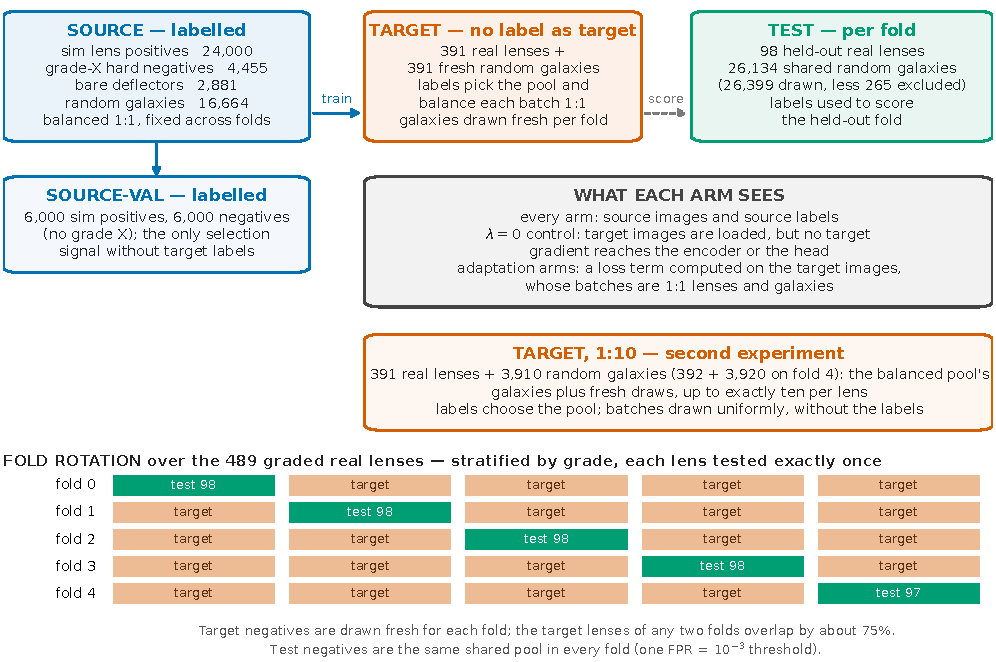
\includegraphics[width=\textwidth]{F1_setup_v6.pdf}
\caption{\textbf{Data roles and fold rotation.} Counts are read from the splits file and, for
the 1:10 target, from its pool file; test negatives are counted after the exclusion of
Section~\ref{sec:testpool}. Target negatives are drawn fresh for each fold; the target lenses of
any two folds overlap by about \rvTargetOverlapPct{}\%. In the main design the catalogue labels
choose the target pool and balance each target batch (Section~\ref{sec:labels}); they are never
a training target. The bottom box is the 1:10 target of the second experiment
(Section~\ref{sec:dilute-methods}): the labels still choose its pool, and its batches are drawn
uniformly, without the labels.}
\label{fig:setup}
\end{figure}

\begin{figure}[t]
\centering
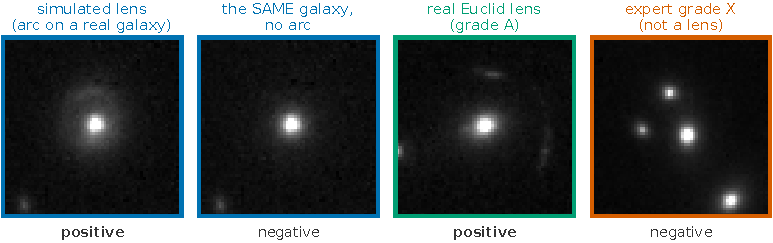
\includegraphics[width=\textwidth]{F2_cutouts.pdf}
\caption{\textbf{One example from each population}, under the per-image stretch the encoder
receives: a simulated lens at the median Einstein radius of its simulation batch, the same
galaxy with no arc,
the grade-A lens at the median expert score, and a grade-X hard negative. Image credit: ESA
Euclid/Euclid Consortium/NASA/Q1-2025.}
\label{fig:cutouts}
\end{figure}

\section{Methods}
\label{sec:methods}

\subsection{Encoder and head}

Every arm uses the Zoobot greyscale encoder~\citep{zoobot}, a ConvNeXt-Nano loaded from the
Hugging Face hub. The Zoobot 2.0 encoders start from ImageNet-12k weights and are trained on
about \zoobotPretrainImages{} Galaxy Zoo--labelled images from ground-based and HST surveys,
none of them Euclid~\citep{walmsley2024scaling}; the greyscale encoder we use was released
later, and its training is not described separately. The encoder returns a 640-dimensional feature
vector. Every arm passes it through a fixed per-dimension standardisation, fitted on cached
source features, before the head. On top sits one head, identical across arms: $\mathrm{LayerNorm}(640)$ followed by a
linear map to a single logit, 1921 trainable parameters. The encoder contains no batch
normalisation and no active dropout, so train and evaluation modes compute the same features.
Appendix~\ref{app:repro} records the software versions.

\subsection{Frozen and unfrozen regimes}

Arms run either \emph{frozen}, with only the head trained, or \emph{unfrozen}, with the top
three timm stages of the encoder trained as well. Because ConvNeXt-Nano is top-heavy, that is
14\,835\,520 trainable encoder parameters, 99.2\% of the encoder, so the unfrozen regime is
close to full fine-tuning; the benchmark fine-tunes the last three blocks of the same
backbone~\citep{lines2025simstosky}, which we implement as these three stages. Unfrozen arms
start from a converged head trained with the encoder frozen and then train the encoder, the order that avoids distorting pretrained features out of
distribution~\citep{kumar2022lpft}. Each unfrozen run is gated at step zero against its head's
recorded value on that fold, which is the check that the run used the right fold.
BNM's pre-registration required both halves of its step-zero gate to match exactly; its runner
applied one positive and $\bnmGateAurocTol{}$ in AUROC, as for DANN. TPR matched exactly on
every fold and AUROC within $\bnmGateAurocBound{}$. All arms
use batch size \rwBatch{} and AdamW. The unfrozen CORAL, DANN, BNM and $\lambda=0$ arms use
the encoder's published fine-tuning defaults (learning rate $\rwOptLr{}$, layer-wise decay
\rwOptDecay{}, weight decay \rwOptWd{}). The unfrozen FreeMatch arm keeps the settings of its
frozen-comparison run (head learning rate $\rwFmHeadLr{}$, encoder learning rate
$\rwFmEncLr{}$, weight decay $\rwFmWd{}$), so that its frozen-to-unfrozen comparison changes
only the encoder setting. Baseline A, which trains only the head, uses learning rate
$\rwBaseLr{}$ and weight decay $\rwBaseWd{}$. We tuned no optimiser setting for any arm, apart
from one comparison: for the CORAL, DANN, BNM and $\lambda = 0$
arms, we compared the encoder's published defaults with one alternative on the development
fold, using the source-only arm, and kept the defaults, which did not score higher. Every step includes a labelled source batch of
\batchSourceRows{} rows, balanced 1:1, next to \batchTargetRows{} target rows in every arm that
loads target images.

\subsection{The arms}
\label{sec:arms}

\paragraph{Baseline A.} Supervised training on the labelled source with the encoder frozen and
no target term. It sees no target image, so one model serves all five folds.

\paragraph{The $\lambda=0$ control.} The DANN arm with its adaptation weight $\lambda$ set to
zero. Target images pass through the discriminator, but the gradient-reversal layer returns
zero gradient, so no target-derived gradient reaches the encoder or the head. The
discriminator itself still trains, and in half precision an overflow in its gradients skips the
whole step; the control skipped \lamSkipFoldTwo{} and DANN \dannSkipFoldTwo{} of 4000 steps on
fold 2, so the control's update schedule is not wholly independent of the target images. DANN and this
control share a head, a budget, a seed and a step grid and differ, in every training-relevant
respect, only in $\lambda$. DANN's confirmatory folds ran with abort conditions armed, while the
control's folds only logged them; no arming condition fired on DANN, and every DANN fold ran its
full 4000 steps. This makes DANN $-$ $\lambda=0$ the only fully controlled pair in this paper. Most other contrasts
also carry one or both of two differences that pairing by fold does not remove. The unfrozen arms start
from three different heads: CORAL from its frozen-comparison heads, FreeMatch from its own,
and DANN, BNM and the control from Baseline A's. Their tuning effort also differs. CORAL's
alignment weight came from a three-point sweep that read only loss magnitudes and feature
statistics. BNM's weight came from a development-fold sweep over a grid set by gradient norms
at step zero; the sweep read the nuclear norm and the predicted-positive fraction, never TPR.
FreeMatch's local-threshold variant was chosen over an alternative by a development-fold
screen of the metric, and DANN carried no tuning. BNM's runner numbers epochs from zero and
DANN's and the control's from one, so on each fold its batches are a different shuffle of the
same source data, and BNM $-$ $\lambda=0$ is not matched in batch order.

\paragraph{BNM.} Batch nuclear-norm maximisation~\citep{cui2020bnm} acts on target predictions
only: no domain comparison, pseudo-label, threshold or discriminator, and one weight,
$\gamma = 0.00787$. Its loss is the nuclear norm divided by $\min(B, C) = \bnmNucDenom{}$, as
in \citeauthor{cui2020bnm}'s code, so $\gamma$ refers to that normalisation. Maximising the nuclear norm of the batch prediction matrix raises both
confidence and prediction diversity~\citep{cui2020bnm}. Before any run, we checked,
analytically and on cached target features, that the objective separates a balanced confident batch from a collapsed one at
our two-class setting.

\paragraph{FreeMatch.} A consistency objective between weakly and strongly augmented target
views, with self-adaptive confidence thresholds and a fairness term~\citep{wang2022freematch}.
We kept FreeMatch's threshold momentum (\fmSatMomentum{}) and fairness weight
(\fmSafWeight{}), but our fairness term compares the mean confident prediction with a fixed
uniform target rather than FreeMatch's running class estimate, and our consistency weight
follows AdaMatch's cosine ramp~\citep{berthelot2022adamatch} over the first half of training,
with no consistency term for the first \fmWarmupPct{}\% of steps; the unfrozen stage starts
after that ramp, so it trains at full weight throughout. Its strong view is the augmentation of
Section~\ref{sec:sim-pipeline}.

\paragraph{DANN.} A domain discriminator behind a gradient-reversal
layer~\citep{ganin2016dann}, mapping $640 \rightarrow 1024 \rightarrow 1024 \rightarrow 1$ with
layer normalisation, ReLU and dropout after each hidden layer; the dropout rate of 0.2 is that
of~\citet{belfiore2024}, and the placement is our choice. The discriminator of \citet{ganin2016dann},
of the same widths, has no normalisation layer; we chose layer rather than batch normalisation so
the discriminator cannot read the domain from batch statistics. It shares the AdamW optimiser,
at learning rate $\dannDiscLr{}$ and weight decay \dannDiscWd{}, without the learning-rate
annealing of \citet{ganin2016dann}. The adaptation weight follows $\lambda = \tanh(5s/2000)$ in the
step $s$ up to step 2000, after which it stays at $\tanh(5)$: their schedule, with training
progress replaced by a fixed horizon of 2000 steps.

\paragraph{CORAL.} We ran the DomainBed variant of correlation
alignment~\citep{gulrajani2021domainbed}, which aligns feature means and covariances rather
than covariances alone~\citep{sun2016coral}. Our head emits a single logit, so we compute the
loss one layer earlier, on the 640-dimensional layer-normalised features, with weight
$\gamma = 16$, after shrinking each covariance \coralShrinkPct{}\% toward a scaled identity; as
in DomainBed, both the mean and covariance terms are averaged over their entries rather than
scaled by \citeauthor{sun2016coral}'s $1/(4d^2)$. With the encoder changing every step, we disabled the running average of the
target covariance.

\subsection{Where labels enter}
\label{sec:labels}

\paragraph{The balanced design.} No real-lens label is ever used as a training target, but
labels shape training in two ways, and we use them a third time for evaluation. First, they
build each fold's target pool: the
$\rvTargetLensPool{}$ graded lenses of the other four folds, without their labels, plus an
equal number of random galaxies. Second, they balance every target batch: our sampler draws
half of each batch from the lens part of the pool and half from the galaxy part, using the
catalogue labels to tell them apart. The DANN, BNM and $\lambda=0$ runs also hold out a
$\rvHoldoutN{}$-image slice of the target pool, chosen half lenses and half galaxies in the
same way, and FreeMatch rebuilds its confidence thresholds from the same balanced loader.
Third, the labels of the held-out fold score the test. Baseline A loads no target images, and
the $\lambda=0$ control passes no target gradient to the encoder or the head, so neither is
trained on the target labels; the control's only dependence on them is through the few
half-precision steps it skips (Section~\ref{sec:arms}). Every adaptation arm does depend on
them. Because the batches are balanced, the class proportion itself reaches every
adaptation objective (Section~\ref{sec:limitations}).

\paragraph{The diluted design.} In our second experiment (Section~\ref{sec:dilute-methods}) the
labels still choose the pool: which \dlPoolLens{} lenses enter it, and the exact count of
\dlRatio{} galaxies per lens (Section~\ref{sec:splits}). Target batches are drawn uniformly at
random from the pool, without the labels, so a batch of \batchTargetRows{} holds about
\dlBatchLens{} lenses on average (about \dlBatchLensTrain{} for DANN and BNM, whose holdout is
removed), and the number varies from batch to batch. The DANN and BNM
runs keep the \dlHoldout{}-image holdout of the balanced design, which is half lenses by
construction, so their training pool is \dlTrainLens{}:\dlTrainGal{}
(\dlTrainLensFour{}:\dlTrainGalFour{} on fold 4) and their batches average a lens fraction of
$\dlTrainFracThree{}$ rather than $\dlPoolFracThree{}$. FreeMatch rebuilds its threshold state
from the uniform sampler.

\paragraph{Why the main design is balanced.} We chose a balanced target because adaptation
failed without one. In early runs with a frozen
encoder and a target far less balanced than the source, DANN and an importance-weighted
variant, IW-CDAN~\citep{zhao2020gls}, both collapsed. On a morphology test (grade-X objects
against random galaxies), alignment lowered the trained head's AUROC from $\rvEarlyNoDa{}$ to
$\rvEarlyDann{}$ for DANN and $\rvEarlyIw{}$ for IW-CDAN, while a linear probe on the same
frozen features reached $\rvEarlyProbe{}$. The information was still in the features, but
alignment removed the head's access to it. Those runs used an earlier pipeline and this proxy
test, and their run artifacts are not in our repository, so we report them as the reason for
the design, not as a result. We then tested part of the design's main weakness
(Section~\ref{sec:results-dilute}): with the encoder unfrozen and a 1:10 target whose batches are
drawn without the labels, DANN keeps a detectable gain over the control, although the comparison
with the balanced target cannot rule out that it lost much of that gain. The early runs differed from these in their frozen encoder,
their pipeline and the degree of imbalance, so the two observations do not contradict each
other.

\subsection{The budget rule}
\label{sec:budget}

We fixed each unfrozen arm's training budget on the development fold, fold 0, and read every arm at its
last checkpoint, so the budget is the model selector. Fold 0 enters no confirmatory number.
BNM's budget came from a rule declared before its development run, and Baseline A's was fixed
before any results; the others were chosen with the development curve in view.
Appendix~\ref{sec:hashes} gives each budget, its basis and its timing. The development fold is
scored against the same shared test negatives as the confirmatory folds, so the budgets we chose
with its curve in view saw those negatives, though none of the confirmatory positives.

\subsection{Pre-registration}
\label{sec:prereg}

We fixed each arm's budget and read-off step before its own confirmatory folds ran, and
hash-protected them then, with four exceptions that rest on our run logs alone
(Appendix~\ref{sec:hashes}). The $\lambda=0$ control was a later addition. On 2026-09-01 we had
decided to run it on the development fold only; on 2026-09-06, after the FreeMatch, CORAL and
DANN confirmatory folds had run, we extended it to folds 1--4, because those arms were unfrozen
and the baseline they were being compared with was not, so their gains could not be attributed
to adaptation. Its budget, read-off rule and decision branches, and the four paired contrasts
against it, were declared and hash-protected before any of its confirmatory folds ran, so the
registration fixes how the control was run and read; the choice of contrasts was made with the
adaptation arms' results known. Appendix~\ref{sec:hashes} lists each file, its digest and its
timing, and the four exceptions.

\subsection{The diluted-target experiment}
\label{sec:dilute-methods}

The second experiment asks whether the gain over the control needs the balanced target. It
changes two things: the target pool, diluted to one lens per \dlRatio{} galaxies
(Section~\ref{sec:splits}), and the sampler, which draws target batches uniformly, without the
labels (Section~\ref{sec:labels}). Nothing else changes: the heads, optimisers, adaptation
weights, seeds, budgets, read-off steps and step-zero gate rules, apart from two tolerances,
are those of the main design, and we retuned nothing.

CORAL and FreeMatch start their unfrozen runs from a head trained with the encoder frozen, so we
reran those frozen stages on the diluted target, with the new pool and sampler and no other
change. Their final heads initialise the unfrozen CORAL and FreeMatch arms, and each unfrozen
run's step-zero gate is taken against its new head. FreeMatch's fold 1, whose balanced run was
gated at an exact tolerance, now uses the one-positive tolerance of the other folds. CORAL's
gate, which in the main design only warned between one positive and \coralGateWarnTpr{} in TPR
or between $\coralGateAurocWarn{}$ and \coralGateAurocAbort{} in AUROC,
now stops a run outside one positive or $\dlGateAurocTol{}$ in AUROC, as for the other arms. DANN and BNM
start from Baseline A's head, as before. We reused the $\lambda=0$ control without rerunning it:
it passes no target gradient to the encoder or the head, so the target pool and sampler enter
what it learns only through the few half-precision steps it skips (Section~\ref{sec:arms}). We
checked that the new sampler shares no random stream with the source sampler or the
augmentation: replaying the samplers alone over the first \dlRngSteps{} training steps of every
arm and fold (for FreeMatch, after its threshold rebuild and warm-up), the source batches under
the new sampler were bit-identical to those under the balanced sampler.

Dilution changes three things at once. It lowers the target's class proportion from 1:1 to
1:\dlRatio{}; it cuts the number of real lenses in a target batch from \dlBatchLensBal{} to
about \dlBatchLens{} (about \dlBatchLensTrain{} for DANN and BNM, whose holdout is removed); and for a fixed number of steps each target lens is seen about
\dlExposureRatio{} times less often. The galaxy side of the target also becomes about
\dlRatio{} times more varied. A change in the gain therefore cannot be attributed to the
proportion alone. The experiment tests whether the gain survives a target far from balanced, as
a first step toward survey prevalence; it does not separate adapting to real images from the
class proportion.

We pre-registered two contrasts per arm, each a paired $t$-interval over folds 1--4 on the
cleaned pool. The primary, $G$, is the diluted run minus the $\lambda=0$ control, with the
control read at 4000 as in the main design's contrasts against the control; for CORAL and FreeMatch,
the same contrast with the control read at the arm's own step is a pre-declared sensitivity
readout. The secondary, $D$, is the balanced run minus the diluted run at the same read-off
step. It carries no verdict, and it includes the noise of a changed batch order. Each arm's
branch follows from $G$ and $D$:
\begin{itemize}
\item \emph{survives}: $G$'s interval excludes zero, and $D$'s includes zero or is negative;
\item \emph{shrinks}: $G$'s interval excludes zero, and $D$'s excludes zero and is positive;
\item \emph{collapses}: $G$'s interval includes zero.
\end{itemize}
Each branch has a fixed sentence, which we report with its numbers filled in
(Section~\ref{sec:results-dilute}). Under \emph{survives}, if $D$'s upper bound exceeds half of
the arm's balanced gain over the control, the sentence must add that the interval admits losing
up to that bound. \emph{Collapses} means only that we cannot detect a gain.

The pre-registration has three parts (Appendix~\ref{sec:hashes}). The first, recorded before
any run, fixes the pool, the sampler, the arms, the contrasts, the branches and our predictions.
The second, recorded after step-zero measurements of at most \dlPartTwoMaxStepsWord{}
training steps per fold, but before any confirmatory run, fixes the step-zero thresholds and which inherited
stop conditions abort a run and which only log. The third was recorded after the first attempt
of CORAL's unfrozen run on fold 1 stopped at its first step (Section~\ref{sec:limitations}), and
before any confirmatory CORAL or FreeMatch unfrozen run. It adds a rule that withholds the verdict from an arm whose run applies fewer than half its
budget's optimiser updates; we set it after a label-free \dlCoralCheckSteps{}-step check in which
CORAL applied \dlCoralCheckAppliedMin{}--\dlCoralCheckAppliedMax{} of \dlCoralCheckSteps{} updates
on every fold, and it fired on no run.
We hashed the analysis plan before computing any value. Appendix~\ref{app:dilute10} gives every
run's skipped updates and applied fraction.

\section{Evaluation}
\label{sec:eval}

\subsection{The metric}

Our primary metric is the true-positive rate at a false-positive rate of $10^{-3}$, written
TPR@$10^{-3}$: we set the threshold so that one non-lens in a thousand is flagged and report the
fraction of real lenses recovered there. We interpolate the ROC curve to FPR${}=10^{-3}$ with
every intermediate point kept. Lens finding has been reported at this
point~\citep{parul2024}, and at lens rarity a false-positive rate near $10^{-3}$ or lower is
needed for a selected sample not to be dominated by non-lenses~\citep{discoveryengineE}. The
metric depends only on the ranking of scores, so it does not depend on the class ratio of the
test pool. We
report AUROC as a secondary check only: with about 26\,000 negatives against 98 positives it
can look healthy while the operating point is poor. The metric is discrete, with a step of
$1/98 \approx 0.010$ on folds 1--3 and $1/97$ on fold 4.

\subsection{Pooling}

Baseline A is one model scoring all five folds, so a single pooled ROC curve is valid for it.
Every adaptation arm trains a different model per fold, so no common threshold exists. We
report those arms as a fold mean with the across-fold standard deviation and always compare
fold mean with fold mean.

\subsection{Intervals and fold dependence}
\label{sec:intervals}

Each comparison is paired: two arms ran on the same folds, so we difference within fold and
report a paired $t$-interval on the four per-fold differences, with $\mathrm{df} = 3$. At
$n = 4$ a bootstrap has at most 35 distinct resamples (256 ordered draws), so we fixed the $t$-interval in
the pre-registration. The frozen comparison (Table~\ref{tab:frozen}) and the FreeMatch
unfrozen $-$ frozen contrast use paired bootstraps instead; we say so where they appear. An
interval that admits zero is not evidence that two arms are equal: it
means this measurement, at four folds and about 98 positives each, cannot separate them.

The four confirmatory folds are not independent. Any two folds share $\rvSharedTargetMin{}$
to $\rvSharedTargetMax{}$ of their $\rvTargetLensPool{}$ target lenses, and every fold uses
the same source set and the same test negatives. Variance estimates that ignore such overlap
between training sets can understate the true variance by a wide
margin~\citep{bengio2004, nadeau2003}, so our intervals are probably too narrow. We expect the
main design's contrasts against the control to survive this, because their intervals sit far
from zero. The narrower comparisons may not, and neither may the dilution experiment's BNM
contrast, whose interval clears zero by \dlGBnmLoAbsThree{}.

\subsection{The contrast set}

Table~\ref{tab:contrasts6} reports \contrastCount{} paired $t$-intervals and one bootstrap interval from the main design, beside
the four primary contrasts of the dilution experiment, at the 95\% level, with no
multiplicity correction; several share a control arm, so they are not independent. Four were
registered with the $\lambda=0$ control, before it ran but after the adaptation arms' results
were known (Section~\ref{sec:prereg}; marked $\dagger$): $\lambda=0$ against Baseline A,
and DANN, CORAL and FreeMatch each against $\lambda=0$, with $\lambda=0$ read at its budget of
4000. The same CORAL and FreeMatch contrasts with $\lambda=0$ read at 2000 and 1500 were
declared with them as sensitivity readouts (marked $\ddagger$). The other contrasts, including
BNM $-$ $\lambda=0$, were not among the four. The dilution experiment
(Section~\ref{sec:dilute-methods}) adds \dlNtWord{} paired $t$-intervals (\dlNtG{} for $G$,
\dlNtD{} for $D$) and \dlNbootWord{} bootstrap intervals, which compare its frozen stages with
those of the main design, again with no multiplicity correction. They share the $\lambda=0$
control with the contrasts above.

\subsection{The test pool, and the change we made after pre-registration}
\label{sec:testpool}

We drew the test negatives from the parent pool before we knew that rounded identifiers hid
duplicates. Matching by exact Euclid ID showed that \DOneLensNeg{} catalogued grade A and B
lenses and \DOneDeflNeg{} simulation host galaxies were among the \TestNegDrawn{} test
negatives. In each fold, $\rvOwnPosMin{}$ to $\rvOwnPosMax{}$ of the \DOneLensNeg{} were that fold's own
test positives, counted a second time as negatives. We wrote and hashed an exclusion rule
(\texttt{rule.json}, self-certifying digest \texttt{\rvRuleSha{}\ldots}) before recomputing anything, applied
it to the stored scores, and retrained nothing. The cleaned pool holds \TestNegDOne{}
negatives, and every number in the main text uses it.

The change raises every arm's TPR, by $\dPoolUpMin{}$ to $\dPoolUpMax{}$, and raises the
adaptation arms the most. On the original pool, the adaptation arms placed $\rvFsevenDaMin{}$
to $\rvFsevenDaMax{}$ of the \DOneLensNeg{} catalogued lenses among the $\rvAboveThrN{}$ negatives above
each fold's threshold, against $\rvFsevenRefMin{}$ to $\rvFsevenRefMax{}$ for Baseline A and
the control. The original pool therefore penalised the stronger models for ranking real
lenses highly. No contrast of the main design changes whether its interval includes zero
(Appendix~\ref{app:prereg_pool}). In the dilution experiment, whose analysis we pre-registered
on the cleaned pool, both forms of FreeMatch's contrast against the control exclude zero on the
original pool (Table~\ref{tab:dl-sensitivity}).

\rwDTwoWord{} of the test lenses also appear in training or validation as negatives: $\rvDTwoRandom{}$ as random galaxies, and one as a bare deflector
that also hosts simulated lenses. Fourteen of them were training negatives and entered the
loss labelled as non-lenses. The other six were validation negatives, which no loss uses.
Removing them changes each arm's fold-mean TPR by at most $\dPoolDTwoMax{}$
(Appendix~\ref{app:prereg_pool}).

\subsection{Secondary readouts and comparability to the benchmark}
\label{sec:eval-comparability}

We also report the completeness at 24\% purity, the operating point of the
benchmark~\citep{lines2025simstosky}. Purity depends on rarity, and our pool is
far denser in lenses than the sky, so we correct it to $N_N/N_P = 2200$, the ratio of objects
searched to lenses found in Q1, which~\citep{lines2025simstosky} adopts and we follow for
comparability, by
\begin{equation}
  \mathrm{purity} \;=\; \frac{\mathrm{TPR}}{\mathrm{TPR} + \mathrm{FPR} \cdot 2200}.
  \label{eq:purity}
\end{equation}
We take the completeness as the largest TPR among thresholds at which the corrected purity is
at least 24\%, since purity need not fall monotonically along the curve; a fold with no such
threshold is n/a, and an arm with an n/a fold has no fold mean and no interval. We
express completeness as a ratio to the benchmark's 0.50.

Lines et al.'s simulation-only model never sees a target image. Our Baseline A and $\lambda=0$
control are comparable to it in that respect, but our adaptation arms are not: they also see
a target built with catalogue labels, balanced 1:1 in the main design and diluted to 1:10 in
the second experiment (Section~\ref{sec:labels}). Their benchmark ratios compare a model given
such a target with one given none. The benchmark's
figure is a mean over ten initialisations with a spread of $\pm 0.10$ in purity, which our
intervals do not include, and its negatives are not matched to ours in depth
(Section~\ref{sec:splits}).

\section{Results}
\label{sec:results}

\subsection{The frozen comparison}
\label{sec:results-frozen}

With the encoder frozen, the two self-training methods reach about twice the TPR of the
source-only baseline (Table~\ref{tab:frozen}, Appendix~\ref{sec:frozen-comparison}): AdaMatch $\dFrozenAda{}$ and FreeMatch
$\dFrozenFm{}$ against $\dFrozenBase{}$, paired differences $\dFrozenAdaDiff{}$
$[\dFrozenAdaLo{}, \dFrozenAdaHi{}]$ and $\dFrozenFmDiff{}$ $[\dFrozenFmLo{}, \dFrozenFmHi{}]$
under the class-conditional paired bootstrap. CORAL sits at $\dFrozenCoral{}$, a difference
from the baseline that excludes zero only at the margin, and the DANN development run scored
exactly what Baseline A scores on the same fold and pool. These arms were not trained under
identical conditions: the feature-space arms ran without augmentation at full precision and the
image-space arms with weak augmentation at half precision (Appendix~\ref{sec:augprec}).
Unfreezing raised FreeMatch's TPR by $\dLpDiff{}$ $[\dLpLo{}, \dLpHi{}]$ (fold-aware paired
bootstrap; Table~\ref{tab:contrasts6}, last row); the frozen and unfrozen FreeMatch runs share
every training setting except the encoder and the 1500 further steps of training, and a
\restartControlStepsNs{}-step frozen continuation tracked the frozen run
(Appendix~\ref{sec:appendix-restart}). It is the only frozen-against-unfrozen contrast we
report; Section~\ref{sec:results-ablation} uses it, with the frozen head's own score, to split
FreeMatch's contrast against the control into the parts gained before and after unfreezing.
The unfrozen arms do not reproduce the
frozen separation between the method families (Section~\ref{sec:results-ablation}), so we treat
that separation as a property of the frozen protocol as we ran it.

\subsection{The main table}
\label{sec:results-main}

Table~\ref{tab:main2} gives the unfrozen arms on folds 1--4. Baseline A and the $\lambda=0$
control both reach $\dFmBaseline{}$, BNM $\dFmBnm{}$, and FreeMatch, DANN and CORAL
$\dFmFreeMatch{}$, $\dFmDann{}$ and $\dFmCoral{}$. Their spreads across folds differ
($\dSdFreeMatch{}$, $\dSdDann{}$ and $\dSdCoral{}$), and at four folds none is well
determined. Baseline A's row is its folds 1--4 mean; its five-fold mean belongs to
Table~\ref{tab:frozen}, and fold 0 enters no confirmatory number.

% GENERATED FILE -- do not edit by hand.
% Rebuild:  python make_all.py (generator: make_main_tables_v2.py)
% Table 2 (rewrite v1): the main table at two decimals. _common.fold_mean on pool D1.
\begin{table}[tbp]
\centering
\caption{\textbf{Main results.} TPR at FPR${}=10^{-3}$ on the cleaned test pool, mean and sample sd over the confirmatory folds 1--4; each arm is read at its final budget except BNM, whose rule gave 1000 steps and which is read at 4000, where its control is read (Appendix~\ref{sec:budget-detail}). Per-fold and four-decimal values: Appendix~\ref{app:perfold}.}
\label{tab:main2}
\footnotesize
\setlength{\tabcolsep}{4pt}
\begin{tabular}{lrrrl}
\toprule
Arm & TPR@$10^{-3}$ & sd & Read at & Encoder \\
\midrule
Baseline A & $0.18$ & $0.03$ & 8000 & frozen \\
$\lambda=0$ control & $0.18$ & $0.03$ & 4000 & unfrozen \\
BNM & $0.40$ & $0.04$ & 4000 & unfrozen \\
FreeMatch & $0.52$ & $0.07$ & 1500 & unfrozen \\
DANN & $0.50$ & $0.17$ & 4000 & unfrozen \\
CORAL & $0.52$ & $0.08$ & 2000 & unfrozen \\
DANN, sensitivity readout & $0.55$ & $0.11$ & 2000 & unfrozen \\
\bottomrule
\end{tabular}
\end{table}


\subsection{What a target signal buys}
\label{sec:results-ablation}

Table~\ref{tab:contrasts6} and Figure~\ref{fig:forest} give the paired contrasts. The three
contrasts against the control, registered before the control ran, are large. DANN $-$ $\lambda=0$ at 4000/4000 is
$\dCtDannLam{}$ $[\dCtDannLamLo{}, \dCtDannLamHi{}]$, CORAL $-$ $\lambda=0$ at 2000/4000 is
$\dCtCoralLamP{}$ $[\dCtCoralLamPLo{}, \dCtCoralLamPHi{}]$, and FreeMatch $-$ $\lambda=0$ at
1500/4000 is $\dCtFmLamP{}$ $[\dCtFmLamPLo{}, \dCtFmLamPHi{}]$; the control starts from
DANN's head, so only the DANN row is a matched contrast, and for CORAL and FreeMatch, which start
from their own heads, it is a method-neutral baseline. Each interval excludes zero,
all four folds agree in sign, and every lower bound lies well above the one-positive step of
the metric. DANN $-$ $\lambda=0$, the fully controlled pair (Section~\ref{sec:arms}), has the
widest interval. Read at the same step as the control, as sensitivity readouts declared with these contrasts,
CORAL gives $\dCtCoralLamM{}$ $[\dCtCoralLamMLo{}, \dCtCoralLamMHi{}]$ at 2000/2000 and FreeMatch
$\dCtFmLamM{}$ $[\dCtFmLamMLo{}, \dCtFmLamMHi{}]$ at 1500/1500; these matched forms remove the
budget difference and leave the other confounds in place (Section~\ref{sec:arms}). BNM,
which was not among the contrasts registered with the control, shares DANN's head but differs
from it in how its adaptation weight was tuned and in batch order (Section~\ref{sec:arms}), and
gives
$\dCtBnmLam{}$ $[\dCtBnmLamLo{}, \dCtBnmLamHi{}]$ at 4000/4000, again with all four folds
agreeing. With a 1:10 target whose batches are drawn
without the labels, DANN and BNM keep a detectable gain over the control, and for CORAL and
FreeMatch we cannot detect one (Section~\ref{sec:results-dilute}).

The
FreeMatch contrast spans two stages of training with a target signal: the unfrozen arm starts
from its frozen-comparison head, which already reaches \rwFiveFmStart{} on these folds, so
\rwFiveFmFrozenPart{} of its $\dCtFmLamP{}$ came with the encoder frozen and
\rwFiveFmUnfrozenPart{} after unfreezing. CORAL's frozen head starts at \rwFiveCoralStart{},
a little above the control's $\dFmLambda{}$. DANN, BNM and the control start from the same head, so
DANN $-$ $\lambda = 0$ and BNM $-$ $\lambda = 0$ each measure a single stage of training; of
the two, only DANN $-$ $\lambda = 0$ differs from the control in nothing but its adaptation
weight (Section~\ref{sec:arms}). The closest prior work finds a gain of the same
kind at the same operating point: Wasserstein alignment took their encoder from 0.0 to 0.241
in TPR at FPR${}=0.1\%$~\citep{parul2024}, on a different survey and test set.

Without a target signal, unfreezing buys nothing we can detect: $\lambda=0$ $-$ Baseline A is
$\dCtLamBase{}$ $[\dCtLamBaseLo{}, \dCtLamBaseHi{}]$. The two arms also differ in augmentation
(Baseline A trains on cached, unaugmented features), training precision, compute venue, code
path and budget, so this row does not isolate unfreezing.

Our starting point is weak. Baseline A and the $\lambda=0$ control reach a TPR of
$\dFmBaseline{}$, and at the benchmark's operating point of 24\% purity Baseline A recovers
$\dLrBaseline{}$\% of the completeness of Lines et al.'s simulation-only model. Their model
differs from ours in its simulations (one of its two simulation sets uses real HST source
galaxies, the other synthetic sources made of one to four S\'ersic components; ours are single-component or
bulge-plus-disk fits), its
negatives and its fine-tuning, and we cannot say which difference accounts for the gap. The
adaptation arms reach $\dLrDaMin{}$--$\dLrDaMax{}$\% of that completeness. What we measure is
therefore a gain over our own simulation-only baseline; whether adaptation would add anything
to a stronger simulation-only model is untested.

The control is one source-only fine-tune, not a tuned best one. The gain does not rest on this
control alone: Baseline A, which never unfreezes, also reaches $\dFmBaseline{}$, and with the
encoder frozen FreeMatch already gains $\dFrozenFmDiff{}$ over the source-only baseline
(Section~\ref{sec:results-frozen}). On the development fold the control ends
below the frozen linear-probe head it started from, at $\dFzLambdaLast{}$ against $\dFzInit{}$
(Figure~\ref{fig:fold0}), the feature distortion that motivates fitting a linear probe before
fine-tuning~\citep{kumar2022lpft}, and a Euclid Q1 transformer retrained on real labels showed a
related drop when fully unfrozen~\citep{astrovink}. That observation rests on one fold, and our statement that
a target signal is needed is relative to this control.

Between objectives, one comparison excludes zero: BNM $-$ CORAL at 2000/2000 is
$\dCtBnmCoral{}$ $[\dCtBnmCoralLo{}, \dCtBnmCoralHi{}]$, with all four folds agreeing. We did
not pre-register it, and it is one of the \contrastCount{} $t$-intervals of the main design, reported
without multiplicity correction. BNM $-$ DANN and BNM $-$
FreeMatch admit zero, and so do DANN $-$ CORAL and DANN $-$ FreeMatch at their declared budgets
and DANN $-$ CORAL at 2000/2000. Section~\ref{sec:resolution} discusses how far these
comparisons can rank the arms.

% GENERATED FILE -- do not edit by hand.
% Rebuild:  python make_all.py (generator: make_dilute10_tables.py)
% Table 2 (paper v6): tables/T3v2_contrasts.tex unchanged, plus the 1:10 block from runs/dilute10_analysis/results.json (G primary).
\begin{table}[tbp]
\centering
\caption{\textbf{Paired contrasts} in TPR at FPR${}=10^{-3}$, folds 1--4, cleaned pool: mean difference, paired $t$-interval (df${}=3$), and the number of folds agreeing in sign. $^{\dagger}$Registered with the $\lambda=0$ control, before it ran but after the adaptation arms' results were known (Section~\ref{sec:prereg}). $^{\ddagger}$Sensitivity readout declared with those contrasts. Steps give where each arm is read. $^{\S}$From the second experiment, with a 1:10 target whose batches are drawn without the labels (Section~\ref{sec:results-dilute}): the arm's diluted run against the same $\lambda=0$ control, pre-registered as that experiment's primary contrast; a bound that rounds to zero at two decimals is shown at three, and the matched-step forms and the balanced $-$ diluted contrasts are in Table~\ref{tab:dl-contrasts4}. Four-decimal values: Tables~\ref{tab:contrasts4} and~\ref{tab:dl-contrasts4}.}
\label{tab:contrasts6}
\footnotesize
\setlength{\tabcolsep}{4pt}
\begin{tabular}{llrrc}
\toprule
Contrast & Steps & $\Delta$ & 95\% CI & Signs \\
\midrule
\multicolumn{5}{l}{\textit{Frozen against unfrozen, no target signal}} \\
$\lambda=0$ $-$ Baseline A$^{\dagger}$ & 4000 / 8000 & $0.00$ & $[-0.09, +0.09]$ & 3/4 \\
\midrule
\multicolumn{5}{l}{\textit{A target signal against none}} \\
DANN $-$ $\lambda=0$$^{\dagger}$ & 4000 / 4000 & $+0.31$ & $[+0.06, +0.57]$ & 4/4 \\
CORAL $-$ $\lambda=0$$^{\dagger}$ & 2000 / 4000 & $+0.34$ & $[+0.19, +0.49]$ & 4/4 \\
FreeMatch $-$ $\lambda=0$$^{\dagger}$ & 1500 / 4000 & $+0.33$ & $[+0.23, +0.44]$ & 4/4 \\
CORAL $-$ $\lambda=0$$^{\ddagger}$ & 2000 / 2000 & $+0.31$ & $[+0.18, +0.43]$ & 4/4 \\
FreeMatch $-$ $\lambda=0$$^{\ddagger}$ & 1500 / 1500 & $+0.32$ & $[+0.20, +0.45]$ & 4/4 \\
BNM $-$ $\lambda=0$ & 4000 / 4000 & $+0.22$ & $[+0.14, +0.30]$ & 4/4 \\
\midrule
\multicolumn{5}{l}{\textit{A target signal against none, 1:10 target}} \\
DANN$^{\S}$ $-$ $\lambda=0$ & 4000 / 4000 & $+0.33$ & $[+0.29, +0.38]$ & 4/4 \\
BNM$^{\S}$ $-$ $\lambda=0$ & 4000 / 4000 & $+0.19$ & $[+0.003, +0.39]$ & 4/4 \\
CORAL$^{\S}$ $-$ $\lambda=0$ & 2000 / 4000 & $+0.01$ & $[-0.03, +0.05]$ & 3/4 \\
FreeMatch$^{\S}$ $-$ $\lambda=0$ & 1500 / 4000 & $+0.25$ & $[-0.004, +0.51]$ & 4/4 \\
\midrule
\multicolumn{5}{l}{\textit{Objective against objective}} \\
BNM $-$ CORAL & 2000 / 2000 & $-0.12$ & $[-0.18, -0.06]$ & 4/4 \\
BNM $-$ DANN & 4000 / 4000 & $-0.09$ & $[-0.31, +0.12]$ & 3/4 \\
BNM $-$ FreeMatch & 1500 / 1500 & $-0.13$ & $[-0.30, +0.03]$ & 4/4 \\
DANN $-$ CORAL & 4000 / 2000 & $-0.02$ & $[-0.22, +0.18]$ & 2/4 \\
DANN $-$ FreeMatch & 4000 / 1500 & $-0.02$ & $[-0.21, +0.17]$ & 2/4 \\
DANN $-$ CORAL & 2000 / 2000 & $+0.03$ & $[-0.07, +0.14]$ & 2/4 \\
\midrule
\multicolumn{5}{l}{\textit{Frozen against unfrozen, same objective (fold-aware paired bootstrap)}} \\
FreeMatch unfrozen $-$ frozen & 1500 / 8000 & $+0.10$ & $[+0.03, +0.17]$ & 4/4 \\
\bottomrule
\end{tabular}
\end{table}


\begin{figure}[t]
\centering
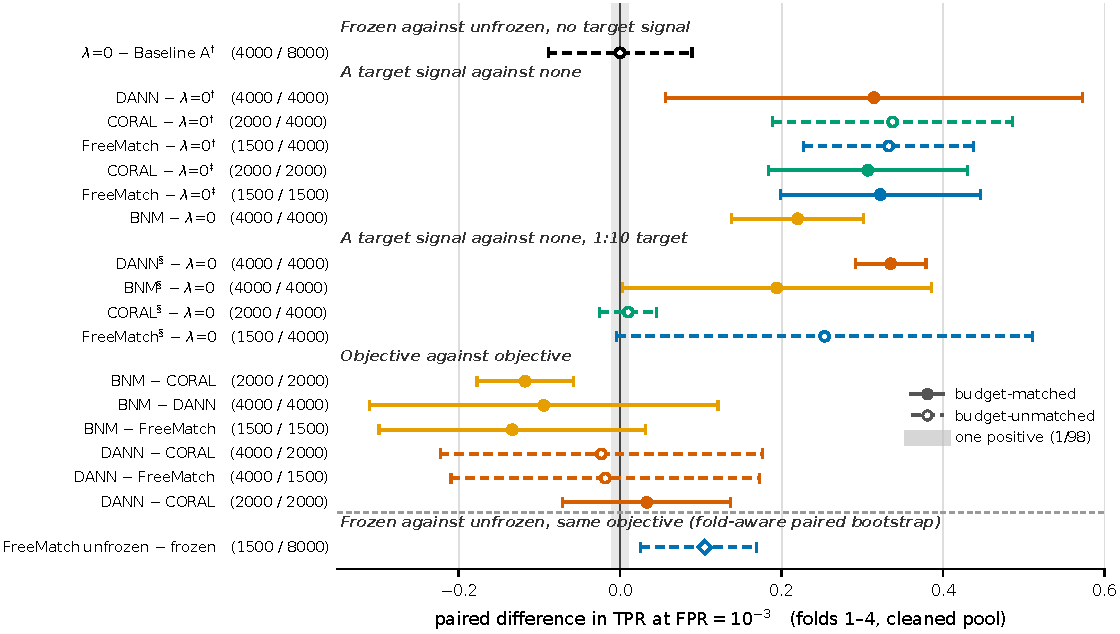
\includegraphics[width=\textwidth]{F3_forest_v6.pdf}
\caption{\textbf{The paired contrasts of Table~\ref{tab:contrasts6}.} Paired $t$-intervals on
four per-fold differences; filled markers are budget-matched, open markers are not.
$^{\dagger}$Registered with the $\lambda=0$ control, before it ran; $^{\ddagger}$sensitivity
readout declared with those contrasts; $^{\S}$from the
second experiment, with a 1:10 target whose batches are drawn without the labels, against the same control
(Section~\ref{sec:results-dilute}). The grey band is one positive ($1/98$). The last row uses
the fold-aware paired bootstrap.}
\label{fig:forest}
\end{figure}

\subsection{A 1:10 target with batches drawn without the labels}
\label{sec:results-dilute}

Table~\ref{tab:dilute} and Figure~\ref{fig:dilute} give the second experiment
(Section~\ref{sec:dilute-methods}). Its four pre-registered branch sentences follow. In these
sentences, as in the pre-registration, ``drawn without the labels'' refers to the target
batches; the pool itself is built from catalogue lenses (Section~\ref{sec:labels}).

\begin{quote}
With a 1:10 target drawn without the labels, DANN still raises TPR@$10^{-3}$ over the control
by $\dlGDannFour{}$ $[\dlGDannLoFour{}, \dlGDannHiFour{}]$, and we detect no loss against the
balanced target ($\dlDDannFour{}$ $[\dlDDannLoFour{}, \dlDDannHiFour{}]$), though the interval
admits losing up to $\dlDDannHiAbsFour{}$ of the original $\dlBalDannAbsFour{}$.

With a 1:10 target drawn without the labels, BNM still raises TPR@$10^{-3}$ over the control by
$\dlGBnmFour{}$ $[\dlGBnmLoFour{}, \dlGBnmHiFour{}]$, and we detect no loss against the balanced
target ($\dlDBnmFour{}$ $[\dlDBnmLoFour{}, \dlDBnmHiFour{}]$), though the interval admits losing
up to $\dlDBnmHiAbsFour{}$ of the original $\dlBalBnmAbsFour{}$.

We cannot detect a gain for CORAL with a 1:10 target: $\dlGCoralFour{}$
$[\dlGCoralLoFour{}, \dlGCoralHiFour{}]$.

We cannot detect a gain for FreeMatch with a 1:10 target: $\dlGFmFour{}$
$[\dlGFmLoFour{},\allowbreak\ \dlGFmHiFour{}]$.
\end{quote}

\noindent With the control read at each arm's own step, CORAL gives $\dlGmCoral{}$
$[\dlGmCoralLo{}, \dlGmCoralHi{}]$ and FreeMatch $\dlGmFm{}$ $[\dlGmFmLo{}, \dlGmFmHi{}]$, the
same branches (Table~\ref{tab:dl-contrasts4}).

The two verdicts closest to zero fall on opposite sides of it by almost nothing: BNM's interval
clears zero by $\dlGBnmLoAbsThree{}$ and FreeMatch's misses it by $\dlGFmLoAbsThree{}$, and
FreeMatch's point estimate is the larger of the two. On the original test pool FreeMatch's
interval excludes zero (Table~\ref{tab:dl-sensitivity}). We do not read the difference between
these two branches as a difference between the methods.

DANN's diluted TPR is $\dlTprDann{}$, against $\dlTprDannBal{}$ with the balanced target. Its
gain over the control on the diluted target, as a fraction of its gain on the balanced one, is
$\dlRetDann{}$, a point estimate only. Its spread across folds is far smaller: an sd of
$\dlSdDann{}$ against $\dlSdDannBal{}$. With one seed per fold, we do not read the narrower spread
as an effect of dilution. For the other arms the same ratio is $\dlRetBnm{}$ for BNM,
$\dlRetFm{}$ for FreeMatch and $\dlRetCoral{}$ for CORAL ($\dlRetmFm{}$ and $\dlRetmCoral{}$ with
the control read at the arm's own step); all are point estimates only.

In point estimates, FreeMatch's smaller diluted gain arises before unfreezing. Its diluted frozen head starts at
$\dlFmStart{}$ against $\dlFmStartBal{}$, a difference of $\dlFmFrozenDiff{}$
$[\dlFmFrozenDiffLo{}, \dlFmFrozenDiffHi{}]$ under the class-conditional paired bootstrap, while
the gain from unfreezing is similar on both targets: $\dlFmUnfrozenPart{}$ against
$\dlFmUnfrozenPartBal{}$ (Table~\ref{tab:dl-frozen}), so its unfrozen stage gains slightly more
on the diluted target than on the balanced one.

CORAL's diluted run differs from its balanced counterpart in more than the target. Its frozen
stage, retrained on the diluted target, ended with a layer-normalisation gain about
\dlCoralGainRatioWord{} times the balanced run's (norm $\dlCoralGainMin{}$--$\dlCoralGainMax{}$
against $\dlCoralGainRoneMin{}$--$\dlCoralGainRoneMax{}$; Table~\ref{tab:dl-heads}), although that
stage's own TPR barely changed ($\dlCoralFrozenDiff{}$
$[\dlCoralFrozenDiffLo{}, \dlCoralFrozenDiffHi{}]$). The unfrozen stage therefore started from
features of norm $\dlCoralFeatStartMin{}$--$\dlCoralFeatStartMax{}$
(Table~\ref{tab:dl-bookkeeping}), which stayed above the guard's threshold of
$\dlCoralCeiling{}$ throughout (minimum $\dlCoralFeatMin{}$), and its ranking quality fell
overall: AUROC $\dlAurocCoral{}$, below its frozen head's $\dlCoralFrozenAuroc{}$
(Table~\ref{tab:dl-frozen}) and the control's $\dlLamAuroc{}$. We cannot tell whether CORAL's diluted run shows no detectable gain
because of the diluted target acting during its unfrozen stage or because of the much larger
head its frozen stage produced on that target.

BNM's predicted-positive fraction on the diluted target batches stayed between
$\dlBnmPpMin{}$ and $\dlBnmPpMax{}$ at every logged step, $\dlBnmPpMean{}$ averaged over every
logged step of the four folds (every \dlBnmPpEvery{} steps, \dlBnmPpN{} per fold), below the
batches' true lens fraction of $\dlBnmLensFrac{}$, rather than drifting upward as we predicted.

We wrote \dlNPredWord{} predictions before any run (Table~\ref{tab:dl-predictions}) and score
them as written. Most failed. We expected DANN's gain to degrade, probably to an interval that
includes zero, and it lost nothing we can detect; we expected CORAL to lose less than DANN,
BNM to lose the most in relative terms, and FreeMatch to lose less than BNM and keep a
detectable gain, and none of these held. The parts that held: CORAL, BNM and
FreeMatch all degraded in point estimate, and FreeMatch's head start shrank. One component,
which our scoring reads as BNM's predicted-positive fraction exceeding $\dlBnmPpThreshold{}$ at
any logged step, holds under that reading, but that reading takes a maximum over \dlBnmPpN{} single-batch
values and would be met by batch noise alone, so we do not count it as support.

The diluted pool is still built from catalogued lenses, and it is far denser in lenses than the
sky (Section~\ref{sec:limitations}).

% GENERATED FILE -- do not edit by hand.
% Rebuild:  python make_all.py (generator: make_dilute10_tables.py)
% Main-text table of the 1:10 experiment. runs/dilute10_analysis/results.json (per_arm, G primary, D, verdicts).
\begin{table}[tbp]
\centering
\caption{\textbf{The 1:10 target, with batches drawn without the labels.} Per arm, folds 1--4, cleaned pool: the diluted run's TPR at FPR${}=10^{-3}$ (mean and sample sd) at the arm's read-off step; $G$, diluted $-$ $\lambda=0$, with the control read at 4000, the primary contrast; $D$, balanced $-$ diluted at the same read-off, secondary and without a verdict; and the pre-registered branch. Paired $t$-intervals (df${}=3$); Signs counts the folds agreeing with $G$'s sign. A bound that rounds to zero at two decimals is shown at three. The $\lambda=0$ control ($\dlLamTpr{}$) is shared with Table~\ref{tab:main2}. Matched-step forms, four-decimal values and per-fold values: Appendix~\ref{app:dilute10}.}
\label{tab:dilute}
\footnotesize
\setlength{\tabcolsep}{4pt}
\begin{tabular}{lrrrrcrl}
\toprule
Arm & Read at & TPR@$10^{-3}$ & sd & $G$, 95\% CI & Signs & $D$, 95\% CI & Branch \\
\midrule
DANN & 4000 & $0.52$ & $0.01$ & $+0.33$ $[+0.29, +0.38]$ & 4/4 & $-0.02$ $[-0.28, +0.24]$ & survives \\
BNM & 4000 & $0.38$ & $0.12$ & $+0.19$ $[+0.003, +0.39]$ & 4/4 & $+0.03$ $[-0.11, +0.16]$ & survives \\
CORAL & 2000 & $0.19$ & $0.04$ & $+0.01$ $[-0.03, +0.05]$ & 3/4 & $+0.33$ $[+0.19, +0.46]$ & collapses \\
FreeMatch & 1500 & $0.44$ & $0.15$ & $+0.25$ $[-0.004, +0.51]$ & 4/4 & $+0.08$ $[-0.08, +0.24]$ & collapses \\
\bottomrule
\end{tabular}
\end{table}


\begin{figure}[t]
\centering
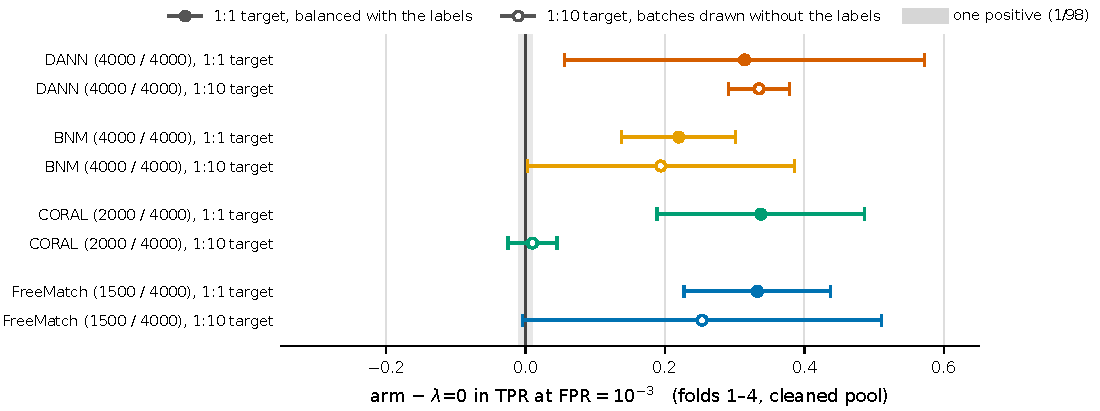
\includegraphics[width=0.92\textwidth]{F7_dilute10.pdf}
\caption{\textbf{The gain over the control with a 1:1 and a 1:10 target.} Per arm, the paired
$t$-interval of the balanced run minus the $\lambda=0$ control (filled) beside that of the
diluted run minus the same control, $G$ (open), folds 1--4, cleaned pool. Each arm is read at
its read-off step (DANN and BNM at \dlReadDann{}, CORAL at \dlReadCoral{}, FreeMatch at
\dlReadFm{}) and the control at 4000 in both. The control is shared: it was run once and is
reused for the 1:10 target, since no target gradient reaches its encoder or head; the target
enters only through the few half-precision steps it skips (Section~\ref{sec:arms}). The grey band is one
positive ($1/98$).}
\label{fig:dilute}
\end{figure}

\subsection{How far CORAL, DANN and FreeMatch can be ranked}
\label{sec:resolution}

At each arm's declared read-off, every paired interval among CORAL, DANN and FreeMatch includes
zero (Tables~\ref{tab:contrasts6} and~\ref{tab:k8pairs6}), so a single checkpoint per arm does
not rank them. Averaging each arm's scores over its last \rwFiveKWord{} checkpoints, the
pre-declared secondary analysis of Appendix~\ref{sec:failed}, FreeMatch has the highest
fold-mean under both score combinations. Its lead over DANN and CORAL excludes zero under the
secondary combination, mean rank, but not under the primary, mean logit
(Table~\ref{tab:k8pairs6}). We read this as a suggestive lead, not an established ranking: it
rests on the secondary combination, our intervals are probably too narrow
(Section~\ref{sec:intervals}), and these are further intervals without correction.

One point estimate per arm carries noise of its own: on a single run, the metric moves from one
checkpoint to the next even when nothing about the method changes. We measured this on the
stored checkpoints of the confirmatory folds. After removing each run's linear trend, the
per-fold scatter is $\rvSigmaMin{}$ to $\rvSigmaMax{}$, and consecutive checkpoints are close
to uncorrelated (lag-1 autocorrelation between $\rvLagMin{}$ and $\rvLagMax{}$). If the two
arms' checkpoint noise were independent, it alone would contribute $\rvNoiseMin{}$ to
$\rvNoiseMax{}$ to a difference of four-fold means; for at least one pair this exceeds the
standard error the paired interval implies, so arms trained on the same folds share much of
their checkpoint noise and the independent figure overstates it
(Appendix~\ref{sec:failed}, Figure~\ref{fig:resolution}). The benchmark likewise finds that, at
this sample size, which lenses are in the test set matters more than the model's
initialisation~\citep{lines2025simstosky}, and sampling theory gives the same direction for
validation sets of this size~\citep{oliver2018realistic}.

\subsection{Operating-point dependence and the benchmark ratio}
\label{sec:results-operating-point}

At 24\% purity the adaptation arms recover, as a share of the benchmark's completeness, CORAL
$\dLrCoral{}$\% $[\dLrCoralLo{}, \dLrCoralHi{}]$, FreeMatch $\dLrFreeMatch{}$\%
$[\dLrFreeMatchLo{}, \dLrFreeMatchHi{}]$, DANN $\dLrDann{}$\% $[\dLrDannLo{}, \dLrDannHi{}]$
and BNM $\dLrBnm{}$\% $[\dLrBnmLo{}, \dLrBnmHi{}]$; Appendix~\ref{app:perfold} gives the
completeness on each fold. One lens moves one fold's ratio by about \dlLensFoldPpWord{}
percentage points and the fold mean by about \dlLensMeanPpWord{} point; the intervals are wide
mainly because the folds differ. No arm's
fold-mean completeness reaches 0.50 at its declared read-off; DANN's sensitivity readout reaches
$\dLrDannSens{}$\%. The $\lambda=0$ control never reaches 24\% purity on two of its folds, so
it has no ratio. On the bright-only test pool, BNM's ratio falls from $\rvBnmDOneRatio{}$ to
$\rvBnmBrightRatio{}$ (Appendix~\ref{app:bright}).

The completeness--purity curves cross (Figure~\ref{fig:comppurity}). FreeMatch runs above
CORAL over $\dEightFmAbovePct{}$\% of the purity range and below it near 24\% purity, so a
single read at that line cannot rank them. AUROC, reported in the appendix tables, saturates:
the $\lambda=0$ control reaches $\dAuLambda{}$ in AUROC and $\dFmLambda{}$ at the operating
point. An unadapted lens finder elsewhere reached an AUROC of 0.921 with a TPR of zero at
FPR${}=0.1\%$~\citep{parul2024}.

\begin{figure}[t]
\centering
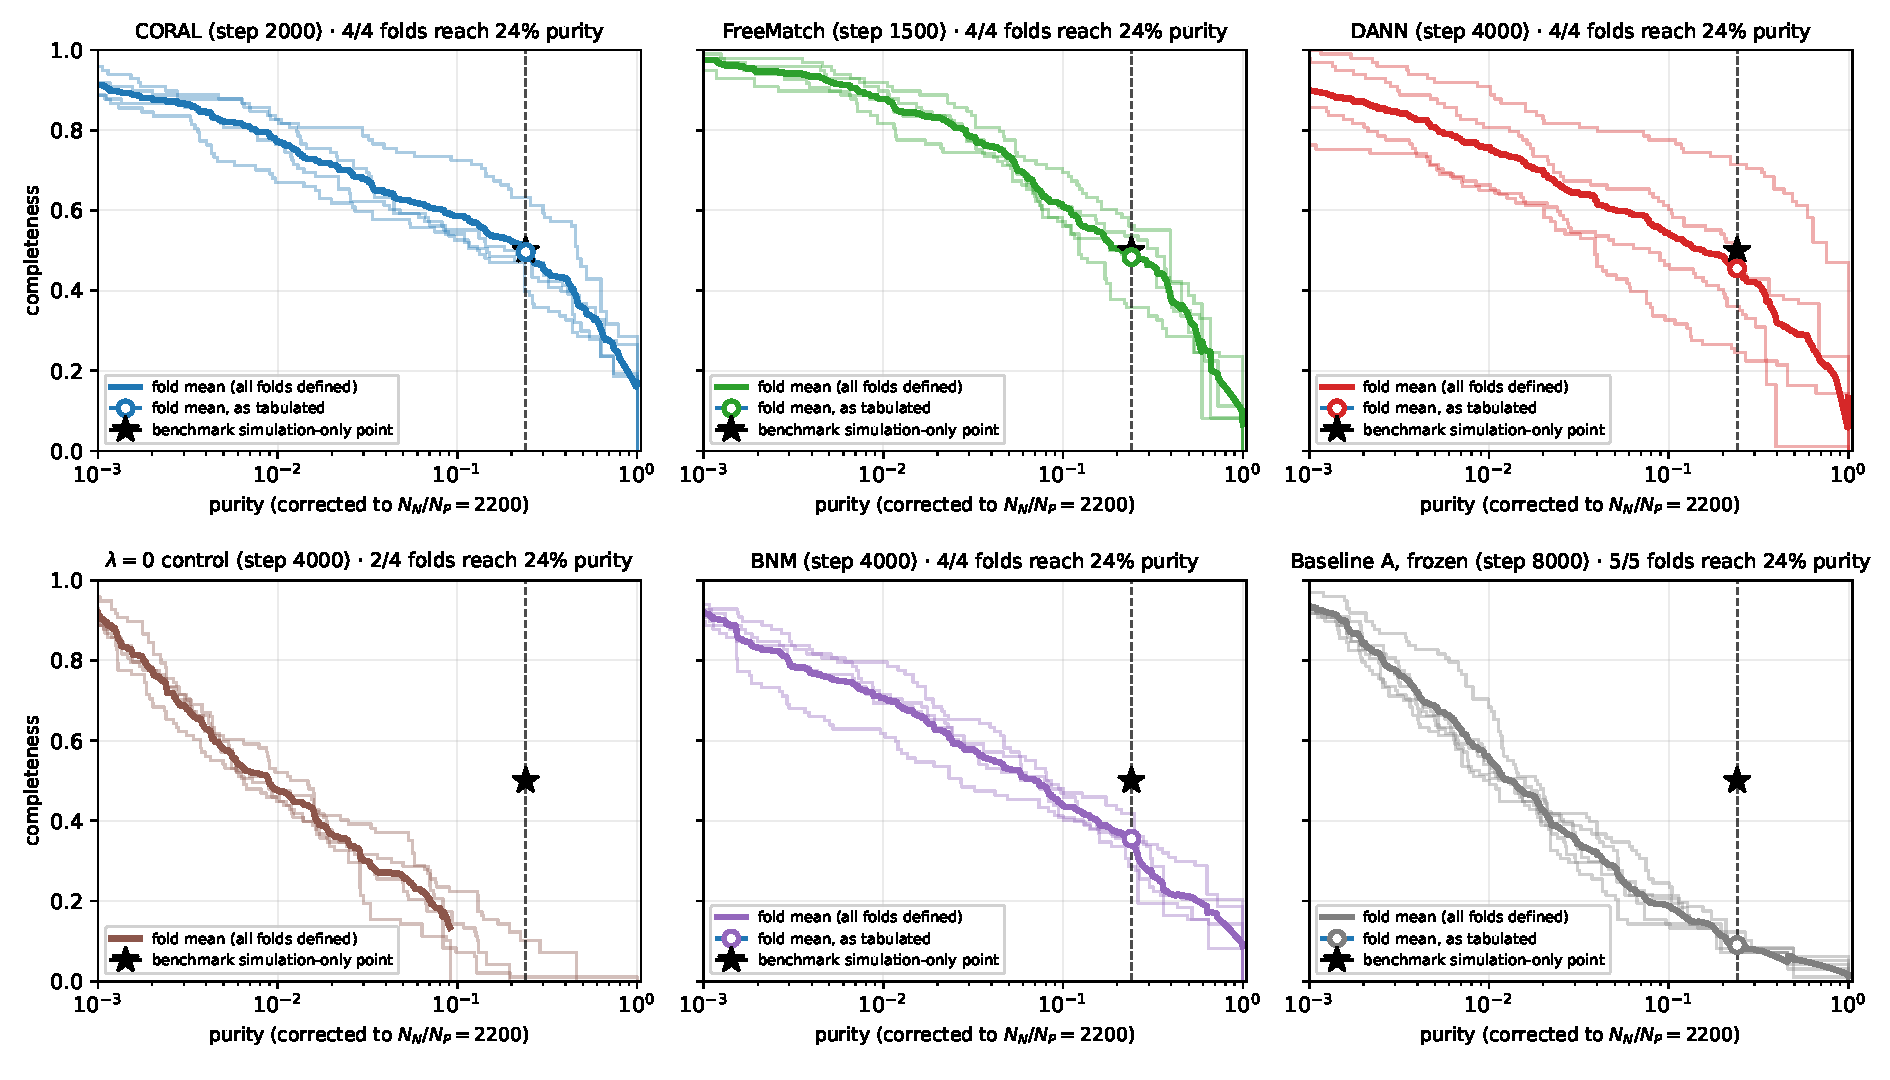
\includegraphics[width=\textwidth]{F6_completeness_purity_v2.pdf}
\caption{\textbf{Completeness against prevalence-corrected purity}, one panel per arm, at the
arm's read-off step; a secondary readout beside the primary TPR@$10^{-3}$. Thin lines are
folds, the thick line the fold mean where every fold is defined, the open circle the tabulated
fold mean, the dashed line 24\% purity and the star the benchmark's simulation-only operating
point. Each panel title gives how many folds reach 24\% purity; a curve that stops before the
dashed line is a fold that never reaches it.}
\label{fig:comppurity}
\end{figure}

\subsection{What the models find and miss}
\label{sec:findmiss}

Every model recovers grade-A lenses about two to three times
($\rvGradeRatioMin{}$ to $\rvGradeRatioMax{}$) as often as grade-B lenses
(Table~\ref{tab:graderecall}). Recall rises with the expert score in every model, and for the
adaptation arms it is lowest for the smallest Einstein radii (Appendix~\ref{app:breakdowns});
modelled Einstein radii exist for $\rvThetaN{}$ of the $\rvConfTestN{}$ confirmatory test
lenses. The lenses that all six models miss (the four adaptation arms, Baseline A and the
control) are mostly grade B ($\rvMissedAllB{}$ of
$\rvMissedAllN{}$), and in the gallery they tend to have small or faint arcs or unusual
configurations (Figure~\ref{fig:gallery}).

The highest-scoring negatives are mostly bright, compact galaxies with extended halos, face-on
spirals, and galaxies with rings or arc-like arms, which are familiar false positives for lens
finders. Of the $\rvTopNegN{}$ negatives that score in the top 30 of any of the seven readouts on any fold,
$\rvTopNegC{}$ are graded C in the Discovery Engine catalogue, the grade below the A and B
cuts that define our positives; none is grade A, B or X. We list the most frequently high-scoring
negatives in Appendix~\ref{app:breakdowns} for inspection and make no claim about their
nature. The \rwAboveN{} negatives above threshold in any cell are brighter than the pool as a
whole: $\rvAboveFaintPct{}$\% are fainter than $I_E = 22.5$, against $\rvPoolFaintPct{}$\% of
all test negatives. Restricting the test negatives to objects brighter than 22.5, the
benchmark's depth, leaves every contrast we recomputed (Table~\ref{tab:bright}) with the same
zero-inclusion (Appendix~\ref{app:bright}).

% GENERATED FILE -- do not edit by hand.
% Rebuild:  python make_all.py (generator: make_main_tables_v2.py)
% Table (rewrite v1): recall by grade, from audit/review_r1/out/A3_recall_by_grade.json.
\begin{table}[tbp]
\centering
\caption{\textbf{Recall by grade} at each fold's FPR${}=10^{-3}$ threshold on the cleaned pool, summed over folds 1--4: recovered/total, rate, and Clopper--Pearson 95\% interval. Descriptive only; no contrast is formed. Per-fold counts: Appendix~\ref{app:breakdowns}.}
\label{tab:graderecall}
\footnotesize
\setlength{\tabcolsep}{4pt}
\begin{tabular}{lrrrrrr}
\toprule
 & \multicolumn{3}{c}{grade A} & \multicolumn{3}{c}{grade B} \\
\cmidrule(lr){2-4}\cmidrule(lr){5-7}
Readout & found & rate & 95\% CI & found & rate & 95\% CI \\
\midrule
Baseline A & 52/196 & $0.27$ & $[0.20, 0.33]$ & 20/195 & $0.10$ & $[0.06, 0.15]$ \\
$\lambda=0$ control & 55/196 & $0.28$ & $[0.22, 0.35]$ & 17/195 & $0.09$ & $[0.05, 0.14]$ \\
BNM & 116/196 & $0.59$ & $[0.52, 0.66]$ & 42/195 & $0.22$ & $[0.16, 0.28]$ \\
FreeMatch & 136/196 & $0.69$ & $[0.62, 0.76]$ & 66/195 & $0.34$ & $[0.27, 0.41]$ \\
DANN & 129/196 & $0.66$ & $[0.59, 0.72]$ & 66/195 & $0.34$ & $[0.27, 0.41]$ \\
DANN, 2000 & 144/196 & $0.73$ & $[0.67, 0.80]$ & 73/195 & $0.37$ & $[0.31, 0.45]$ \\
CORAL & 139/196 & $0.71$ & $[0.64, 0.77]$ & 65/195 & $0.33$ & $[0.27, 0.40]$ \\
\bottomrule
\end{tabular}
\end{table}


\begin{figure}[t]
\centering
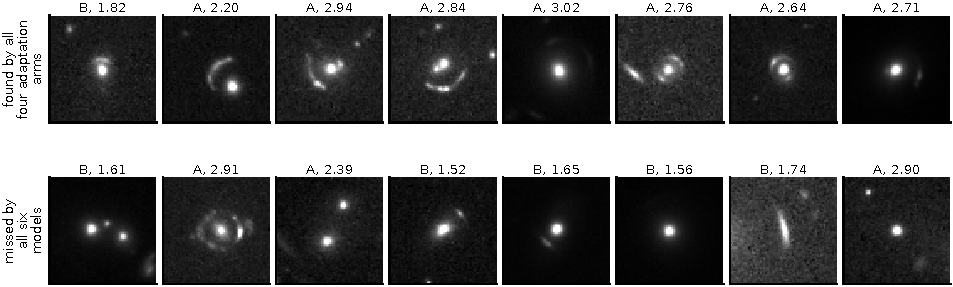
\includegraphics[width=\textwidth]{FY_lens_gallery.pdf}
\caption{\textbf{Confirmatory test lenses found and missed.} Top: the first eight, by Euclid
ID, recovered by all four adaptation arms; bottom: the first eight missed by all six models
(the four adaptation arms, Baseline A and the control). Each
panel gives the grade and expert score, under the encoder's input stretch. Image credit: ESA
Euclid/Euclid Consortium/NASA/Q1-2025.}
\label{fig:gallery}
\end{figure}

\section{Negative results}
\label{sec:negative}

\paragraph{Checkpoint selection without labels.} We tested six signals for choosing a
checkpoint without target labels, scoring each by the TPR it loses against the best checkpoint
on the development fold, over nine development runs. Source-validation AUROC and purity
saturate from the first checkpoint and carry no information. The norm of the head's gradient,
proposed as a model-internal diagnostic~\citep{headgradnorm}, points in opposite directions on
different methods. All but one signal fell inside the range
of a random choice around our rule of taking the last checkpoint. The exception,
source-validation TPR, was the best selector on one unfrozen run and the worst on the other,
and nothing without labels tells the two cases apart, so we kept the last checkpoint. These are
development-fold values on the original test pool, and three of the signals could not be
computed on the unfrozen runs because their per-checkpoint files were lost.

\paragraph{Budget peak and decay onset are unmeasurable.} On the development fold the peak of
the FreeMatch curve cannot be located, since the steps within two positives of the best are
spread from \rwFzStepMin{} to \rwFzStepMax{}, and the onset of decay is detectable only at the
8000-step cap (Table~\ref{tab:orderings2}, rows 1 and 2). Appendix~\ref{sec:budget-detail}
describes how we fixed each budget instead.

\paragraph{The memorisation diagnostic is inconclusive.} Each fold's target pool holds about
782 images, few enough for an unfrozen encoder to memorise. We pre-declared a diagnostic: the
gap in a nuclear-norm statistic between a target slice an arm trains on and the held-out slice.
On BNM the gap resolves under one declared reading and not under the reading we declared
primary. On the $\lambda=0$ control, where neither slice is trained on, its scatter is larger
than the effect it is meant to bound. CORAL and FreeMatch have no held-out slice. DANN and its
control share one and differ only in $\lambda$; computed on their stored checkpoints in a
retrospective analysis whose rule we declared before computing it, DANN's gap minus the control's is
$\mzPrim{}$ $[\mzPrimLo{}, \mzPrimHi{}]$ at the read-off step and, as the secondary reading,
$\mzSec{}$ $[\mzSecLo{}, \mzSecHi{}]$ averaged over checkpoints (Table~\ref{tab:dl-memorisation});
both intervals are without multiplicity correction and probably too narrow, because the folds'
target pools overlap (Section~\ref{sec:intervals}).
Re-drawing the random augmentation of the same images moved one fold's gap by
$\mzViewShift{}$, as large as the effects the diagnostic is meant to detect, so we computed these
values without augmentation. They are not comparable with BNM's gap, which used one
augmented view per image. Whether part of the adaptation gain comes from fitting these
particular images therefore remains undetermined.

\paragraph{Our predictions for the dilution experiment.} Most components of the \dlNPredWord{}
predictions we recorded before the 1:10 runs failed; Section~\ref{sec:results-dilute} scores them.

\begin{figure}[t]
\centering
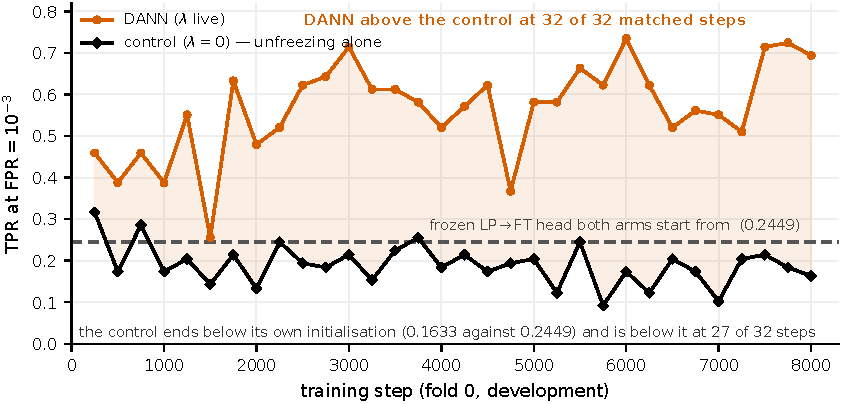
\includegraphics[width=\textwidth]{F4_fold0_curves.pdf}
\caption{\textbf{The $\lambda=0$ control and DANN on the development fold}, identical at step 0
and differing only in $\lambda$. The dashed line is the frozen linear-probe head both start
from. The control ends below it. One fold; it enters no headline number.}
\label{fig:fold0}
\end{figure}

\section{Limitations}
\label{sec:limitations}

\paragraph{The target and its labels.} This is the deepest limitation. In our main design each
fold's target pool is built from the graded lenses of the other folds and an equal number of
random galaxies, and every target batch is balanced 1:1 using the catalogue labels
(Section~\ref{sec:labels}). A search on new survey data has no graded lenses to build such a
pool from; it would face the survey's own rarity, about one lens found per 2200 objects
searched~\citep{lines2025simstosky}. Our dilution experiment
removes the balancing of the batches but keeps a pool built from catalogue lenses, and its
1:\dlRatio{} is still about \dlDenserWord{} times denser in lenses than the survey's 1:2200; we
tested no target at survey prevalence, so our results do not transfer unaltered to that
setting. The dilution changes more than the proportion (Section~\ref{sec:dilute-methods}). It ran one ratio, with one seed per fold, and CORAL's diluted run is entangled
with the head its frozen stage produced (Section~\ref{sec:results-dilute}). The theory that
motivated balancing covers marginal alignment, which is CORAL and
DANN here~\citep{zhao2019invariant, zhao2020gls}, and a benchmark finds such methods fragile
under shifts in class proportions~\citep{classimbalanceda}; it does not speak directly to FreeMatch or
BNM, and we applied the balanced target to every arm to keep the comparison matched. The
closest precedent shares the constraint: its balanced target of 1754 lenses and 1754
non-lenses is also built from known lens candidates~\citep{parul2024}.

Balancing is not the only remedy for differing class proportions. \citet{zhao2020gls} estimate
the class ratio between domains from the source confusion matrix and the target predictions,
then reweight the adversarial and classification losses by it, which needs no target label. We
tried one such method, IW-CDAN, only in early frozen runs with an imbalanced target, where it
collapsed together with DANN (Section~\ref{sec:labels}). Label-shift estimation methods that
need no target labels, such as re-estimating the class prior by
expectation--maximisation~\citep{saerens2002} or black-box shift
estimation~\citep{lipton2018}, are a natural next step.

\paragraph{What the target signal contains.} Because every target batch of the main design is
half lenses and half galaxies, the adaptation arms see not only real images but a known class
proportion, and each
objective can use it: BNM's diversity term favours a batch whose predictions split evenly,
FreeMatch's fairness term targets a uniform class marginal, and DANN and CORAL align the
target's feature distribution with that of the balanced source. Learning from groups of
unlabelled examples whose class proportions are known has been studied as a learning problem in
its own right~\citep{quadrianto2009}. The $\lambda = 0$ control removes both the target images'
gradient and this proportion, apart from the few half-precision steps it skips
(Section~\ref{sec:arms}), so our contrasts cannot say how much of the gain comes from
adapting to real images and how much from the known proportion. The dilution experiment answers
this only in part. DANN keeps a detectable gain over the control without batches balanced 1:1
(Section~\ref{sec:results-dilute}), although the comparison with the balanced target cannot
rule out that it lost much of its gain. Every objective still sees a target whose composition
we fixed with the labels, and FreeMatch's fairness term still assumes a uniform class mix, so
we still cannot separate adapting to real images from the class proportion.

\paragraph{The diluted runs' numerics.} CORAL's unfrozen stage on the diluted target skipped its
first \dlCoralSkipMin{}--\dlCoralSkipMax{} optimiser updates on every fold, before its loss
scaling settled, and none after, so it applied at least \dlCoralAppliedPct{}\% of its budget's
updates. Its inherited
feature-norm guard, which our pre-registration made advisory, fired on every step. Its first
attempt on fold 1 stopped at step 1 on that guard, an implementation error that produced no
data, and the third part of our pre-registration permitted the rerun
(Appendices~\ref{sec:prereg-dilute} and~\ref{app:dilute10}).

\paragraph{A weak simulation-only baseline.} Our simulation-only baseline recovers
$\dLrBaseline{}$\% of the benchmark's completeness, so the
gains we report are measured from a low starting point, against a control that is itself one
source-only fine-tune (Section~\ref{sec:results-ablation}).

\paragraph{When the control was added.} The control and its contrasts were added after the
adaptation arms' results were known; its own runs were pre-registered, but the decision to make
those comparisons was not (Section~\ref{sec:prereg}).

\paragraph{Fold dependence, four folds and one seed.} Every interval rests on four folds whose
target pools overlap (Section~\ref{sec:intervals}). Every reported result comes from a single
run per fold with one seed, so seed variance is not separated from fold variance anywhere. The
ranking analysis of Section~\ref{sec:resolution} is approximate for the same reason.

\paragraph{Test negatives and depth.} \FracFaintTest{}\% of our test negatives are fainter
than the benchmark's limit of
$I_E = 22.5$ (Section~\ref{sec:splits}). Some may be lenses: the exact-ID audit found
catalogued lenses in the original pool, and $\rvTopNegC{}$ of the highest-scoring negatives in
the cleaned pool are grade-C
candidates (Section~\ref{sec:findmiss}). Restricting the pool to the benchmark's depth leaves
every contrast we recomputed (Table~\ref{tab:bright}) with the same zero-inclusion
(Appendix~\ref{app:bright}), but purity values are
not directly comparable with the benchmark's. Our positives were found mostly by
machine-learning finders, one of them built on Zoobot, the encoder we use, so recall on them may
overstate recall on lenses such finders miss~\citep{lines2025discoveryengineC, discoveryengineA}.

\paragraph{The simulations.} Our lensed sources are parametric profiles fitted to COSMOS
galaxies, so they lack the clumps and irregular structure of real high-redshift sources; in HST
imaging only about a fifth of galaxies are fully described by such
models~\citep{mandelbaum2014great3}. The deflector velocity dispersions follow a local
($z \lesssim 0.1$) velocity dispersion function, while our deflectors lie at a median redshift
of \simZlMedian{}, and we apply no evolution. \DeflUnphysN{} deflectors carry catalogue values outside the
physical range ($\log M_* > \DeflUnphysMass{}$ or an absolute VIS magnitude below $\DeflUnphysMag{}$),
and \DeflUnphysDrawn{} of these host \DeflUnphysLenses{} of the simulated lenses.

\paragraph{Software.} We did not pin or record the versions of \texttt{timm} and GalSim used in
training and simulation (Appendix~\ref{app:repro}).

\section{Conclusion}
\label{sec:conclusion}

We measured what unsupervised domain adaptation adds to a simulation-trained lens finder on
Euclid Q1, at the false-positive rate a search runs at. With a class-balanced target, each of
four published objectives raised the TPR at FPR${}=10^{-3}$ from $\dFmBaseline{}$ to between
$\dHeadMin{}$ and $\dHeadMax{}$, measured against a control that differs from one of them only
in its adaptation weight. Because the target batches are balanced, that signal includes a known
class proportion as well as real images, and our design cannot separate the two. In a second
pre-registered experiment, a first test toward survey prevalence, we diluted the target to one
lens per ten galaxies and drew its batches without the labels. DANN still raised TPR over the
control, by $\dlGDann{}$ $[\dlGDannLo{}, \dlGDannHi{}]$, and BNM by $\dlGBnm{}$
$[\dlGBnmLoThree{}, \dlGBnmHi{}]$, though for both the comparison with the balanced target
cannot rule out that much of the original gain was lost; for CORAL and FreeMatch we cannot detect a gain. We
could not establish a ranking of CORAL, DANN and FreeMatch: at their declared read-offs every
paired interval includes zero, and an \rwFiveKWord{}-checkpoint average favours FreeMatch with an
interval excluding zero under only one of its two pre-declared score combinations. Settling the
ranking needs more graded lenses rather than another read-off convention. Two conditions limit how far
these numbers carry. Our simulation-only baseline is weak, so the gains are measured from a low
starting point. And every target we used, the diluted one included, is built from a lens
catalogue that a new survey will not have, and is far denser in lenses than the sky. The next
experiment is a target with no catalogue in it at all: random galaxies drawn from the survey, at
its own prevalence, which removes the remaining use of the labels and the remaining gap in lens
density.


\section*{Acknowledgements}
% The two sentences below are required verbatim: the first by the Euclid Q1 data licence
% (ESA Cosmos, "Q1 Data License and Credits"), the second because ESA Datalabs was used
% (scripts/filter_deflectors_leakfree.py, scripts/probe_size_native.py,
% scripts/extract_neg_ids.py). See paper/CREDITS_PROVENANCE_REPORT.md.
This work has made use of the Euclid Q1 data from the Euclid mission of the European Space
Agency (ESA), 2025, \url{https://doi.org/10.57780/esa-2853f3b}~\citep{euclidq1data}.
This research makes use of ESA Datalabs (datalabs.esa.int;~\cite{navarro2024datalabs}), an initiative by ESA's Data
Science and Archives Division in the Science and Operations Department, Directorate of
Science.

GPU time was provided by Kaggle and Google Colab.

We used Anthropic's Claude (claude.ai and Claude Code) throughout this work: to help design
the experiments and their pre-registrations, to write and test the training and analysis code,
and to draft and revise the text. Every number in the paper is generated by scripts from stored
run artifacts and recomputed against them at every build (\nCrossChecks{} automated checks), and
each analysis was checked against known-null controls and against exact reproductions of earlier
results before new values were computed (Appendices~\ref{sec:hashes} and~\ref{app:repro}). These
checks were themselves written with the same tools. We read and revised all text and code and
take full responsibility for the content.

This work used PyTorch~\citep{paszke2019pytorch}, timm~\citep{wightman2019timm},
NumPy~\citep{harris2020numpy}, SciPy~\citep{virtanen2020scipy},
scikit-learn~\citep{pedregosa2011sklearn}, Matplotlib~\citep{hunter2007matplotlib} and
Astropy~\citep{astropy2022}; we also used GalSim~\citep{rowe2015galsim} and
lenstronomy~\citep{birrer2018lenstronomy,birrer2021lenstronomy}.

\section*{Data and code availability}
The code for simulation, training, evaluation and every table and figure in this paper is
available at \url{https://github.com/NavneetAdaval/euclid-q1-lens-adaptation} and archived at
\url{https://doi.org/10.5281/zenodo.24285258}. For \dlLostArmsWord{} of the 1:10 arms (DANN, BNM and the CORAL and FreeMatch frozen
stages), the exact versions of \dlLostFilesWord{} helper scripts that ran
(\texttt{dilute10\_common.py}, \texttt{dilute10\_batch\_log.py} and the arm's wrapper) are lost;
the release has their later versions. Their recorded digests are in the run files. For
Baseline A, FreeMatch and CORAL's balanced frozen stage, the runs recorded no per-module digests,
and BNM's balanced runs recorded only the files its pre-registration hashes. The
repository includes the pre-registration and budget files with their recorded digests
(Appendix~\ref{sec:hashes}), the pre-fold copy of the DANN pre-registration, the split
definitions, and the stored test scores from which the reported numbers are computed:
at each checkpoint for the unfrozen confirmatory runs of both experiments, and at the final
checkpoint for the frozen runs, together with the summary files the frozen comparison and the
secondary analyses read; for DANN's frozen development run only its summary file is kept. It
also includes the definition file of the 1:10 target pool (Section~\ref{sec:splits}) and the
list of negatives removed from the test pool (Section~\ref{sec:testpool}). Our run logs, the
dated lab notes we kept throughout this work, are not part of the release. Every digest and
value the build takes from them is in \texttt{public\_inputs/\allowbreak record\_extract.json},
which also records the logs' own digest, and we will share the logs with the editor and
referees on request. The
Euclid images are not redistributed. The negatives come from the Euclid Q1 data release,
available through the ESA Euclid Science Archive, and the lens positives from the public
Q1 lens-cutout archives~\citep{discoveryenginecat}; the split definitions identify the negatives by Euclid object
identifier and the lens positives through a list of their Euclid identifiers, and the
repository includes the retrieval and preprocessing code. The simulated training lenses
are painted onto these images and are likewise not redistributed; the generator that
produced them is included with its fixed seed, but an exact regeneration is not
guaranteed, because neither the GalSim version used (Section~\ref{sec:limitations}) nor
the number of parallel workers the generator ran with was recorded. The Datalabs query that
selected the deflectors was not archived; the released identifier list defines the sample.
The lens positives are the grade A and B
candidates of Euclid Collaboration: Walmsley et al.~\citep{discoveryengineA}. The grade-X hard negatives are identified through
version 0.0.1 of the Discovery Engine catalogue~\citep{discoveryenginecat001}; later versions
publish grades A--C only~\citep{discoveryenginecat}. The pretrained encoder is the Zoobot checkpoint
named in Appendix~\ref{app:repro}, available from the Hugging Face hub.

% \nocite{*} was removed at stage 3, with the prose in place and every reference cited
% from a sentence. Rewrite v1 (2026-10-10) removed every entry the rewritten text no longer
% cites; paper/REWRITE_v1_REPORT.md lists them, and the previous refs.bib is in
% backup/rewrite_v1_20261010_182859/paper/.
%
% plainnat_doi_eprint.bst is plainnat.bst with two changes, listed at the top of that file:
% @misc entries print their doi, and every entry with an eprint prints its arXiv identifier.
\bibliographystyle{plainnat_doi_eprint}
\bibliography{refs}

% The appendices follow the references (A&A, MNRAS and OJAp order). placeins puts a
% \FloatBarrier before every \section, so each appendix's tables stay inside it.
\appendix
\section{Per-fold values and four-decimal tables}
\label{app:perfold}

This appendix gives the fold-level values behind every aggregate in the main text at four
decimals, so that each can be recomputed by hand. Table~\ref{tab:contrasts4} is the four-decimal
version of Table~\ref{tab:contrasts6}, with each contrast's budget-match status; the per-fold
tables give TPR, AUROC, completeness at 24\% purity and purity at 50\% completeness for every
readout, with their fold-means.

% GENERATED FILE -- do not edit by hand.
% Rebuild:  python make_all.py (generator: make_appendix_tables_v2.py)
% Appendix A (rewrite v2): tables/T2_contrasts.tex's rows (make_t2_contrasts.py, protected), reordered and marked as Table 3; number tokens asserted identical.
\begin{table}[htbp]
\centering
\caption{\textbf{Paired contrasts at four decimals}, folds 1--4, cleaned pool. Paired $t$-interval on the four per-fold differences (df${}=3$); the last row uses the fold-aware paired bootstrap ($B=5000$). Signs counts the folds agreeing in direction with the mean. $^{\dagger}$Registered with the $\lambda=0$ control, before it ran; $^{\ddagger}$sensitivity readout declared with those contrasts. The arms differ in head initialisation and tuning (Section~\ref{sec:arms}), and a budget match removes only the budget difference. \contrastCount{} intervals at 95\%, with no multiplicity correction; several share the control arm. $^{*}$Interval excludes zero.}
\label{tab:contrasts4}
\footnotesize
\setlength{\tabcolsep}{4pt}
\begin{tabular}{llrlcl}
\toprule
Contrast & Steps & $\Delta$ TPR@$10^{-3}$ & 95\% CI & Signs & Budget \\
\midrule
\multicolumn{6}{l}{\textit{Frozen against unfrozen, no target signal}} \\
$\lambda=0$ $-$ Baseline A$^{\dagger}$ & 4000 / 8000 & $0.0000$$^{a}$ & $[-0.0890, +0.0889]$ & 3/4 & --- \\
\midrule
\multicolumn{6}{l}{\textit{A target signal against none}} \\
DANN $-$ $\lambda=0$$^{\dagger}$ & 4000 / 4000 & $+0.3144$$^{*}$ & $[+0.0565, +0.5722]$ & 4/4 & matched \\
CORAL $-$ $\lambda=0$$^{\dagger}$ & 2000 / 4000 & $+0.3375$$^{*}$ & $[+0.1889, +0.4860]$ & 4/4 & unmatched \\
FreeMatch $-$ $\lambda=0$$^{\dagger}$ & 1500 / 4000 & $+0.3325$$^{*}$ & $[+0.2272, +0.4378]$ & 4/4 & unmatched \\
CORAL $-$ $\lambda=0$$^{\ddagger}$ & 2000 / 2000 & $+0.3068$$^{*}$ & $[+0.1834, +0.4301]$ & 4/4 & matched \\
FreeMatch $-$ $\lambda=0$$^{\ddagger}$ & 1500 / 1500 & $+0.3223$$^{*}$ & $[+0.1984, +0.4463]$ & 4/4 & matched \\
BNM $-$ $\lambda=0$ & 4000 / 4000 & $+0.2199$$^{*}$ & $[+0.1383, +0.3014]$ & 4/4 & matched \\
\midrule
\multicolumn{6}{l}{\textit{Objective against objective}} \\
BNM $-$ CORAL & 2000 / 2000 & $-0.1176$$^{*}$ & $[-0.1772, -0.0580]$ & 4/4 & matched \\
BNM $-$ DANN & 4000 / 4000 & $-0.0945$ & $[-0.3104, +0.1214]$ & 3/4 & matched \\
BNM $-$ FreeMatch & 1500 / 1500 & $-0.1334$ & $[-0.2986, +0.0319]$ & 4/4 & matched \\
DANN $-$ CORAL & 4000 / 2000 & $-0.0231$ & $[-0.2227, +0.1765]$ & 2/4 & unmatched \\
DANN $-$ FreeMatch & 4000 / 1500 & $-0.0182$ & $[-0.2092, +0.1729]$ & 2/4 & unmatched \\
DANN $-$ CORAL & 2000 / 2000 & $+0.0331$ & $[-0.0711, +0.1372]$ & 2/4 & matched \\
\midrule
\multicolumn{6}{l}{\textit{Frozen against unfrozen, same objective (fold-aware paired bootstrap)}} \\
FreeMatch unfrozen $-$ frozen & 1500 / 8000 & $+0.1049$$^{*}$ & $[+0.0256, +0.1687]$ & 4/4 & --- \\
\bottomrule
\end{tabular}

\vspace{2pt}
\footnotesize $^{a}$$-0.00003$ before rounding.
\end{table}


% GENERATED FILE -- do not edit by hand.
% Rebuild:  python make_all.py (generator: make_appendix_relabel_v2.py)
% Relabelled copy of tables/T5_perfold.tex; tabular number tokens asserted identical, caption/notes token changes declared.
\begin{table}[htbp]
\centering
\caption{\textbf{Per-fold values: TPR at FPR${}=10^{-3}$ (primary).} Rows marked
\footnotesize(sens.)\normalsize{} are pre-declared readouts reported beside the headline, not instead of it; the row marked
\footnotesize(own budget)\normalsize{} is BNM's rule-derived budget, which matches no other arm's, so it is reported for BNM alone. The fold-0 column is
\textbf{development} and enters no mean; it is populated only for the single
frozen Baseline A model. \emph{n/a} marks a value the metric leaves undefined,
and an arm with any undefined fold gets no fold-mean.}
\label{tab:perfold-tpr2}
\footnotesize
\setlength{\tabcolsep}{4pt}
\begin{tabular}{lrrrrrrrr}
\toprule
Arm & Step & fold 0$^{\dagger}$ & fold 1 & fold 2 & fold 3 & fold 4 & mean & sd \\
\midrule
Baseline A & 8000 & $0.2449$ & $0.1429$ & $0.2143$ & $0.1735$ & $0.2062$ & $0.1842$ & $0.0327$ \\
$\lambda=0$\,\footnotesize(sens.) & 1500 & \emph{n/a} & $0.2245$ & $0.1735$ & $0.1837$ & $0.1959$ & $0.1944$ & $0.0221$ \\
$\lambda=0$\,\footnotesize(sens.) & 2000 & \emph{n/a} & $0.2245$ & $0.2245$ & $0.1735$ & $0.2371$ & $0.2149$ & $0.0282$ \\
$\lambda=0$ & 4000 & \emph{n/a} & $0.2245$ & $0.1735$ & $0.1429$ & $0.1959$ & $0.1842$ & $0.0346$ \\
BNM\,\footnotesize(own budget) & 1000 & \emph{n/a} & $0.4082$ & $0.4592$ & $0.3265$ & $0.4845$ & $0.4196$ & $0.0697$ \\
BNM\,\footnotesize(sens.) & 1500 & \emph{n/a} & $0.4082$ & $0.5204$ & $0.3469$ & $0.2577$ & $0.3833$ & $0.1103$ \\
BNM\,\footnotesize(sens.) & 2000 & \emph{n/a} & $0.3776$ & $0.5000$ & $0.3367$ & $0.4021$ & $0.4041$ & $0.0694$ \\
BNM & 4000 & \emph{n/a} & $0.3980$ & $0.4592$ & $0.3776$ & $0.3814$ & $0.4040$ & $0.0378$ \\
FreeMatch & 1500 & \emph{n/a} & $0.5000$ & $0.5918$ & $0.4286$ & $0.5464$ & $0.5167$ & $0.0697$ \\
DANN\,\footnotesize(sens.) & 2000 & \emph{n/a} & $0.5714$ & $0.7041$ & $0.5000$ & $0.4433$ & $0.5547$ & $0.1125$ \\
DANN & 4000 & \emph{n/a} & $0.5408$ & $0.7143$ & $0.3163$ & $0.4227$ & $0.4985$ & $0.1706$ \\
CORAL & 2000 & \emph{n/a} & $0.4694$ & $0.6327$ & $0.5000$ & $0.4845$ & $0.5216$ & $0.0751$ \\
\bottomrule
\end{tabular}

\vspace{2pt}
\footnotesize $^{\dagger}$fold 0 is the development fold and is excluded from
every confirmatory mean in this paper; \emph{n/a} in that column means the arm has no
fold-0 run on this grid, not that the value is undefined.
\end{table}

\begin{table}[htbp]
\centering
\caption{\textbf{Per-fold values: AUROC (secondary, saturating sanity metric).} Rows marked
\footnotesize(sens.)\normalsize{} are pre-declared readouts reported beside the headline, not instead of it; the row marked
\footnotesize(own budget)\normalsize{} is BNM's rule-derived budget, which matches no other arm's, so it is reported for BNM alone. The fold-0 column is
\textbf{development} and enters no mean; it is populated only for the single
frozen Baseline A model. \emph{n/a} marks a value the metric leaves undefined,
and an arm with any undefined fold gets no fold-mean.}
\label{tab:perfold-auroc2}
\footnotesize
\setlength{\tabcolsep}{4pt}
\begin{tabular}{lrrrrrrrr}
\toprule
Arm & Step & fold 0$^{\dagger}$ & fold 1 & fold 2 & fold 3 & fold 4 & mean & sd \\
\midrule
Baseline A & 8000 & $0.9439$ & $0.8937$ & $0.9045$ & $0.9031$ & $0.8922$ & $0.8984$ & $0.0063$ \\
$\lambda=0$\,\footnotesize(sens.) & 1500 & \emph{n/a} & $0.8931$ & $0.8952$ & $0.8738$ & $0.8878$ & $0.8875$ & $0.0097$ \\
$\lambda=0$\,\footnotesize(sens.) & 2000 & \emph{n/a} & $0.8874$ & $0.8791$ & $0.8905$ & $0.9187$ & $0.8939$ & $0.0172$ \\
$\lambda=0$ & 4000 & \emph{n/a} & $0.8728$ & $0.8674$ & $0.8776$ & $0.9084$ & $0.8815$ & $0.0184$ \\
BNM\,\footnotesize(own budget) & 1000 & \emph{n/a} & $0.9521$ & $0.9332$ & $0.8890$ & $0.9412$ & $0.9289$ & $0.0277$ \\
BNM\,\footnotesize(sens.) & 1500 & \emph{n/a} & $0.9274$ & $0.9475$ & $0.9222$ & $0.8729$ & $0.9175$ & $0.0317$ \\
BNM\,\footnotesize(sens.) & 2000 & \emph{n/a} & $0.9026$ & $0.9318$ & $0.8728$ & $0.9047$ & $0.9030$ & $0.0241$ \\
BNM & 4000 & \emph{n/a} & $0.9314$ & $0.9039$ & $0.9058$ & $0.8974$ & $0.9096$ & $0.0150$ \\
FreeMatch & 1500 & \emph{n/a} & $0.9499$ & $0.9768$ & $0.9688$ & $0.9710$ & $0.9666$ & $0.0117$ \\
DANN\,\footnotesize(sens.) & 2000 & \emph{n/a} & $0.9274$ & $0.9552$ & $0.9020$ & $0.9457$ & $0.9326$ & $0.0234$ \\
DANN & 4000 & \emph{n/a} & $0.9544$ & $0.9815$ & $0.8672$ & $0.8272$ & $0.9076$ & $0.0725$ \\
CORAL & 2000 & \emph{n/a} & $0.9168$ & $0.9401$ & $0.8922$ & $0.8896$ & $0.9097$ & $0.0237$ \\
\bottomrule
\end{tabular}

\vspace{2pt}
\footnotesize $^{\dagger}$fold 0 is the development fold and is excluded from
every confirmatory mean in this paper; \emph{n/a} in that column means the arm has no
fold-0 run on this grid, not that the value is undefined.
\end{table}

\begin{table}[htbp]
\centering
\caption{\textbf{Per-fold values: completeness at 24\% purity (secondary; Lines et al.'s operating point).} Rows marked
\footnotesize(sens.)\normalsize{} are pre-declared readouts reported beside the headline, not instead of it; the row marked
\footnotesize(own budget)\normalsize{} is BNM's rule-derived budget, which matches no other arm's, so it is reported for BNM alone. The fold-0 column is
\textbf{development} and enters no mean; it is populated only for the single
frozen Baseline A model. \emph{n/a} marks a value the metric leaves undefined,
and an arm with any undefined fold gets no fold-mean. $\lambda=0$'s fold-4 value at step 4000 is \lamFourCompLenses{} lens.}
\label{tab:perfold-comp2}
\footnotesize
\setlength{\tabcolsep}{4pt}
\begin{tabular}{lrrrrrrrr}
\toprule
Arm & Step & fold 0$^{\dagger}$ & fold 1 & fold 2 & fold 3 & fold 4 & mean & sd \\
\midrule
Baseline A & 8000 & $0.0816$ & $0.1224$ & $0.0714$ & $0.0816$ & $0.0928$ & $0.0921$ & $0.0220$ \\
$\lambda=0$\,\footnotesize(sens.) & 1500 & \emph{n/a} & $0.0816$ & $0.0612$ & \emph{n/a} & $0.0309$ & \emph{n/a} & \emph{n/a} \\
$\lambda=0$\,\footnotesize(sens.) & 2000 & \emph{n/a} & $0.1224$ & $0.0612$ & $0.0408$ & \emph{n/a} & \emph{n/a} & \emph{n/a} \\
$\lambda=0$ & 4000 & \emph{n/a} & $0.1020$ & \emph{n/a} & \emph{n/a} & $0.0103$ & \emph{n/a} & \emph{n/a} \\
BNM\,\footnotesize(own budget) & 1000 & \emph{n/a} & $0.3673$ & $0.3571$ & $0.2449$ & $0.4639$ & $0.3583$ & $0.0896$ \\
BNM\,\footnotesize(sens.) & 1500 & \emph{n/a} & $0.3163$ & $0.4898$ & $0.3061$ & $0.0825$ & $0.2987$ & $0.1670$ \\
BNM\,\footnotesize(sens.) & 2000 & \emph{n/a} & $0.3469$ & $0.4694$ & $0.2959$ & $0.3608$ & $0.3683$ & $0.0730$ \\
BNM & 4000 & \emph{n/a} & $0.3571$ & $0.4184$ & $0.2857$ & $0.3608$ & $0.3555$ & $0.0543$ \\
FreeMatch & 1500 & \emph{n/a} & $0.4796$ & $0.5612$ & $0.3571$ & $0.5361$ & $0.4835$ & $0.0909$ \\
DANN\,\footnotesize(sens.) & 2000 & \emph{n/a} & $0.5408$ & $0.7041$ & $0.4592$ & $0.4124$ & $0.5291$ & $0.1282$ \\
DANN & 4000 & \emph{n/a} & $0.5000$ & $0.7143$ & $0.2449$ & $0.3608$ & $0.4550$ & $0.2019$ \\
CORAL & 2000 & \emph{n/a} & $0.3980$ & $0.6327$ & $0.4796$ & $0.4742$ & $0.4961$ & $0.0984$ \\
\bottomrule
\end{tabular}

\vspace{2pt}
\footnotesize $^{\dagger}$fold 0 is the development fold and is excluded from
every confirmatory mean in this paper; \emph{n/a} in that column means the arm has no
fold-0 run on this grid, not that the value is undefined.
\end{table}

\begin{table}[htbp]
\centering
\caption{\textbf{Per-fold values: purity at 50\% completeness, corrected to $1{:}2200$.} Rows marked
\footnotesize(sens.)\normalsize{} are pre-declared readouts reported beside the headline, not instead of it; the row marked
\footnotesize(own budget)\normalsize{} is BNM's rule-derived budget, which matches no other arm's, so it is reported for BNM alone. The fold-0 column is
\textbf{development} and enters no mean; it is populated only for the single
frozen Baseline A model. \emph{n/a} marks a value the metric leaves undefined,
and an arm with any undefined fold gets no fold-mean.}
\label{tab:perfold-purity2}
\footnotesize
\setlength{\tabcolsep}{4pt}
\begin{tabular}{lrrrrrrrr}
\toprule
Arm & Step & fold 0$^{\dagger}$ & fold 1 & fold 2 & fold 3 & fold 4 & mean & sd \\
\midrule
Baseline A & 8000 & $0.0186$ & $0.0132$ & $0.0100$ & $0.0138$ & $0.0158$ & $0.0132$ & $0.0024$ \\
$\lambda=0$\,\footnotesize(sens.) & 1500 & \emph{n/a} & $0.0224$ & $0.0096$ & $0.0063$ & $0.0063$ & $0.0112$ & $0.0077$ \\
$\lambda=0$\,\footnotesize(sens.) & 2000 & \emph{n/a} & $0.0138$ & $0.0068$ & $0.0077$ & $0.0153$ & $0.0109$ & $0.0043$ \\
$\lambda=0$ & 4000 & \emph{n/a} & $0.0147$ & $0.0088$ & $0.0064$ & $0.0081$ & $0.0095$ & $0.0036$ \\
BNM\,\footnotesize(own budget) & 1000 & \emph{n/a} & $0.1008$ & $0.1265$ & $0.0303$ & $0.1545$ & $0.1030$ & $0.0532$ \\
BNM\,\footnotesize(sens.) & 1500 & \emph{n/a} & $0.0772$ & $0.2205$ & $0.0483$ & $0.0216$ & $0.0919$ & $0.0887$ \\
BNM\,\footnotesize(sens.) & 2000 & \emph{n/a} & $0.0619$ & $0.1920$ & $0.0311$ & $0.0915$ & $0.0941$ & $0.0697$ \\
BNM & 4000 & \emph{n/a} & $0.0862$ & $0.0826$ & $0.0734$ & $0.0271$ & $0.0673$ & $0.0273$ \\
FreeMatch & 1500 & \emph{n/a} & $0.2126$ & $0.3726$ & $0.1214$ & $0.3311$ & $0.2594$ & $0.1143$ \\
DANN\,\footnotesize(sens.) & 2000 & \emph{n/a} & $0.3136$ & $0.8559$ & $0.2052$ & $0.1155$ & $0.3726$ & $0.3323$ \\
DANN & 4000 & \emph{n/a} & $0.2481$ & $0.7481$ & $0.0383$ & $0.0831$ & $0.2794$ & $0.3252$ \\
CORAL & 2000 & \emph{n/a} & $0.1322$ & $0.4590$ & $0.2126$ & $0.1487$ & $0.2381$ & $0.1513$ \\
\bottomrule
\end{tabular}

\vspace{2pt}
\footnotesize $^{\dagger}$fold 0 is the development fold and is excluded from
every confirmatory mean in this paper; \emph{n/a} in that column means the arm has no
fold-0 run on this grid, not that the value is undefined.
\end{table}


\section{The budget rule, pre-registration hashes and amendments}
\label{sec:hashes}

\subsection{The budget rule}
\label{sec:budget-detail}

We fixed the budget of every arm except Baseline A on a development run on fold 0: BNM's by a
rule declared before that run, which reads its nuclear norm (the $\gamma$ sweep on the same fold
had already indicated that the rule would give about \bnmBudgetPreview{} steps, and it gave
\bnmBudgetSteps{}); the others with its TPR curve in view. Baseline A's 8000 steps were fixed before any results existed. We read each arm at its
last checkpoint, so the training budget is the model selector. Every confirmatory run
reached its arm's final budget. BNM's ran to 4000 steps so that all its readouts came from one
run; no part of its training depends on the total number of steps, so its step-1000 checkpoint
is the model a 1000-step run would produce. For some arms we stated the budget as a rule derived
from the arm's configuration: 4000 for DANN, twice its $\lambda$
horizon; 4000 for the $\lambda=0$ control, read where its treatment is read; and 1000 for BNM,
twice the step at which its nuclear norm reaches an analytic ceiling. Baseline A uses 8000, the
matched budget of the frozen comparison. For CORAL we declared 2000 on cost, declining the
development curve's maximum at 2500. For FreeMatch we first declared 2000 on robustness
grounds, with the development curve in view, and later amended it to 1500, the development
curve's highest point, although Section~\ref{sec:negative} shows that this maximum is poorly
located. Only \rwBudgetPreCurve{} were fixed before the corresponding
development curve existed; the others were chosen with that curve in view. BNM's 1000 matches
no other arm's budget, so we read it at 4000, the step of its control. Where we compare two arms
at the same step, a budget match removes only the budget confound; the head and tuning
differences of Section~\ref{sec:arms} remain.

\subsection{Pre-registration}
\label{sec:prereg-detail}

We fixed each arm's budget and read-off step before its own confirmatory folds ran and, except
for the four items below, hash-protected them then. The $\lambda=0$ control's folds 1--4 and the
four paired contrasts against it came later (Section~\ref{sec:prereg}): on 2026-09-01 we recorded
in the DANN pre-registration that the control would be reported from the development fold alone
(key \texttt{arm1\_folds\_1\_4\_declined}), and on 2026-09-06, after the FreeMatch, CORAL and
DANN confirmatory folds had run, we reversed that decision. The control's own pre-registration
precedes all its confirmatory folds, but we chose its contrasts knowing the adaptation arms'
results.
Two versions of our private Kaggle dataset hold copies of these files. Their dates are the
version dates shown on the dataset page, which we read ourselves; a reader cannot check them, so
they corroborate our account but are not independent timestamps. One holds the DANN declaration
(see below). The other, dated \lambdaKaggleDate{}, before the $\lambda = 0$ control's first
confirmatory fold, holds that control's pre-registration, which fixes the four paired contrasts
against it, and the pre-registration's audit; both match their recorded digests. Four items rest on our run logs alone, which are not distributed (Data and code
availability): Baseline A's budget, fixed
before any results in our first frozen comparison, which predates our hash protection; the
precedence of one DANN prediction over its development-fold test; the timing of BNM's budget;
and FreeMatch's amended budget, whose hash file did not survive. We evaluated every condition
declared for the $\lambda=0$ control at step zero, and across its whole development run, before
writing it into the pre-registration. Fold 0 enters no confirmatory number: every contrast and
every unfrozen-arm mean uses folds 1--4, 391 test positives in all.

Table~\ref{tab:hashes6} lists every pre-registration and budget file with its digest, re-derived
from disk when the paper is built. We record amendments beside a hashed file rather than
rewriting it.

% GENERATED FILE -- do not edit by hand.
% Rebuild:  python make_all.py (generator: make_dilute10_tables.py)
% Appendix B (paper v6): tables/A2_hashes_v2.tex unchanged, plus the 1:10 experiment's declarations, digests re-derived from disk through scripts/integrity.py.
\begin{table}[htbp]
\centering
\caption{\textbf{Protected artifacts and when each was recorded.} Each enrolled file is made read-only once written and is checked by digest at every build. \emph{Recorded} is the file's own timestamp; where it has none, \emph{Source} says whether its timing rests on a flag inside the file, on a dated Kaggle dataset version, or on our run logs alone. \emph{vs.\ runs} compares it with the start of the first confirmatory run it governs. Two kinds of digest are checked: a whole-file digest, and a self-certifying digest of the file body with its own hash field removed. \emph{Enrolled} says whether the file is in the inventory that every analysis run re-checks; every row's digest, enrolled or not, matches its file when the table is built. Fourteen artifacts are hashed; thirteen are re-checked by every analysis run, and the window-averaging declaration is hashed but not enrolled. The 1:10 rows are dated against that experiment's first run. The DANN pre-registration has two rows, its archived pre-fold copy and the file as regenerated after the folds. A date without a time is a day-only record. The last row is protected but governs no run.}
\label{tab:hashes6}
\scriptsize
\setlength{\tabcolsep}{4pt}
\begin{tabular}{>{\TRAG}p{2.6cm}>{\TRAG}p{1.3cm}>{\TRAG}p{1.75cm}>{\TRAG}p{1.3cm}>{\TRAG}p{1.3cm}>{\TRAG}p{1.4cm}l>{\TRAG}p{1.4cm}}
\toprule
Artifact & Recorded (UTC) & Source & First run (UTC) & vs.\ runs & Digest & sha256 (first 16) & Enrolled \\
\midrule
BNM budget & --- & run logs only & 2026-09-14 11:36 & not checkable & whole file & \texttt{5b92e161ed1e301f} & yes \\
BNM pre-registration & --- & file (flag only) & 2026-09-14 11:36 & before (flag) & whole file & \texttt{d205f6784213b75d} & yes \\
CORAL budget & 2026-08-21 18:01 & file & 2026-08-23 12:42 & before & self-certifying & \texttt{65c20810485968d8} & yes \\
DANN budget + sensitivity readout & 2026-09-02 & file & 2026-09-03 13:54 & before & self-certifying & \texttt{abf0dae0e313ae53} & yes \\
DANN pre-registration, pre-fold copy & 2026-09-02 16:26 & archived copy & 2026-09-03 13:54 & before & self-certifying & \texttt{51351308196ad332} & no (archived) \\
DANN pre-registration, regenerated file & 2026-09-05 11:43 & file & 2026-09-03 13:54 & \textbf{after} & self-certifying & \texttt{3ad1fc361a150b95} & yes \\
$\lambda=0$ control pre-registration & --- & Kaggle dataset version, 6 Sept 2026 & 2026-09-07 08:38 & before & self-certifying & \texttt{c1694a479eafb040} & yes \\
Checkpoint-window averaging declaration & --- & file (flag only) & --- & before (flag) & self-certifying & \texttt{a572b81e4c730590} & \textbf{no} \\
\midrule
\multicolumn{8}{l}{\emph{The 1:10 diluted-target experiment (Section~\ref{sec:dilute-methods}):}} \\
1:10 pool definition & --- & digest in part 1 & 2026-10-13 18:58 & before & whole file & \texttt{18c73d6c1cbad99e} & yes \\
1:10 pre-registration, part 1 & 2026-10-13 13:19 & file & 2026-10-13 18:58 & before & self-certifying & \texttt{bd537a025e81833e} & yes \\
1:10 pre-registration, part 2 & 2026-10-13 18:07 & file & 2026-10-13 18:58 & before & self-certifying & \texttt{b8e09197a204be83} & yes \\
1:10 pre-registration, part 3 & 2026-10-19 14:13 & file & 2026-10-20 16:10 & before & self-certifying & \texttt{1b583ea2ae5056ed} & yes \\
\multicolumn{8}{l}{\emph{Analysis declarations (govern analyses, not runs):}} \\
1:10 analysis plan & 2026-10-23 18:45 & file & --- & n/a & self-certifying & \texttt{68367e25c784334c} & yes \\
DANN $-$ $\lambda=0$ memorisation plan (retrospective) & --- & run logs only & --- & n/a & self-certifying & \texttt{9dee7d6a02c17be0} & yes \\
\midrule
\multicolumn{8}{l}{\emph{Protected, not a pre-registration (governs no run):}} \\
BNM step-0 gradient norms, re-measured & --- & run logs only & --- & n/a & whole file & \texttt{04930f2fe924b99a} & yes \\
\bottomrule
\end{tabular}
\end{table}

\begingroup\footnotesize\noindent\textbf{Notes to Table~\ref{tab:hashes6}.} What each file fixed: 
\emph{BNM budget}: budget 1000, BNM's rule-derived budget. The file carries no timestamp and no before-flag, so its timing rests on our run logs alone.
\emph{BNM pre-registration}: the weight $\gamma$. BNM's weight came from a development-fold sweep over a grid set by gradient norms at step zero; the sweep read the nuclear norm and the predicted-positive fraction, never TPR. The budget was left undecided, because its rule reads a crossing only the development run produces.
\emph{CORAL budget}: budget 2000, declared on cost, declining the development curve's maximum.
\emph{DANN budget and sensitivity readout}: budget 4000, $2 \times$ the $\lambda$ horizon, and the step-2000 sensitivity declaration, which we call the headline-and-sensitivity rule: the headline is the mean at 4000, and the mean at step 2000 is a budget-sensitivity check reported beside the headline, not instead of it. Every confirmatory fold records this file's self-certifying digest when it starts, so the rule is verified as fixed before the folds. The declaration says ``5-fold mean'', but the same file excludes fold 0 from every headline, and we report folds 1--4; with the development fold, the five-fold means on the cleaned pool are \dDannFiveFoldFourK{} at 4000 and \dDannFiveFoldTwoK{} at 2000.
\emph{DANN pre-registration}: the arms, the abort conditions, the rule for declaring the margin $M$, the budget decision, the headline-and-sensitivity rule, and the predictions, among them the arc-suppression prediction and the spread prediction. We regenerated the file after the folds; the first row is the copy that predates them, and every one of its \dannPrefoldIdenticalKeys{} pre-fold keys is unchanged in the second. The copy is entry \dannPrefoldEntry{} of the file's hash history, and we archive it in the repository; the regeneration, on 2026-09-05, added \dannPrefoldAddedKeys{} keys reporting fold results. The copy does not establish that the arc-suppression prediction preceded its own development-fold test, whose outcome it already contains; entry \dannArcEntry{} of the hash history was not recovered.
\emph{$\lambda=0$ control pre-registration}: budget 4000, under the rule that the control is read where its treatment is read; three outcome branches (low, near the adaptation arms, in between), which decided whether BNM would run, with no run by default; and the four paired contrasts against the control. The file's description of two other arms' budgets is wrong: it attributes FreeMatch's 1500 to the saturation of its adaptive threshold, which completes 90\% of its rise on the development fold only at step \fmTauNinetyStep{}, and CORAL's 2000 to its configuration. Appendix~\ref{sec:budget-detail} gives the bases recorded at the time (FreeMatch: the development curve's highest point; CORAL: cost). The sentence governs nothing in the control's run.
\emph{Checkpoint-window averaging declaration}: $k=8$ primary, the grid $\{1,2,4,8\}$, both score combinations, and a window that ends at each arm's read-off step; it governs analyses, not training runs.
\emph{BNM step-0 gradient norms, re-measured}: a second, later measurement. The $\gamma$ grid is never re-derived from it, and its original measuring run is lost. Protected, but not a pre-registration: it governs no run.
A further digest in our run logs, \texttt{7356acda\ldots}, is the hash of a superseded pre-registration text; the text is lost, and we keep its digest in \texttt{public\_inputs/\allowbreak record\_extract.json}. The window-averaging row, marked \emph{no} under \emph{Enrolled}, is hashed in our run logs, and its digest matches the file, but it is absent from the inventory that every analysis run re-checks, so it has neither the re-check nor the read-only protection of the other thirteen. We did not enrol it after the fact, because that would date its protection to the writing of this paper. The first 1:10 run was CORAL's frozen stage on fold 1, run locally.\par\endgroup


\paragraph{The DANN pre-registration.} We recorded it in our run logs on 2026-08-26 and amended
it there on 2026-08-28 and 2026-08-30. Its machine-readable file is regenerated whole by its
writer and was last written on 2026-09-05, after DANN's confirmatory folds, so that file's own
hash dates only the regeneration. A copy of the file as it stood on 2026-09-02, before the
folds, survives in a private Kaggle dataset version dated 2 September 2026, and we archive it in
the repository. Its digest, \texttt{\dannPrefoldSha{}\ldots}, is entry \dannPrefoldEntry{} of the file's hash
history, its
recorded time precedes the first confirmatory fold, and every one of its
\dannPrefoldIdenticalKeys{} pre-fold keys is identical in the current file; the
regeneration added \dannPrefoldAddedKeys{} keys reporting fold results. This copy therefore
verifies, before the confirmatory folds, the spread prediction, the headline and sensitivity
rule, the budget, the abort conditions as we re-specified them on 2026-08-30 from the fold-0
control and development runs (the file labels that change derived, not pre-registered; it made
two conditions advisory, so it could stop no run), and every other key. It does not verify two things. The first is the precedence of the
arc-suppression prediction over its own development-fold test: the prediction is dated
2026-08-30 in our run logs, but the 2 September copy already contains its outcome, resolved on
2026-09-01, and the earlier file state (history entry \dannArcEntry{}) was not recovered; the
prediction was falsified. The second is the content of the file's states before 2 September,
history entries 1--9. The step-2000 sensitivity rule is also verifiable through the separate
DANN budget file, which predates the folds and whose digest every confirmatory fold recorded
when it started.

\paragraph{The FreeMatch budget amendment.} We amended FreeMatch's budget from 2000 to 1500
steps, the development curve's highest point, although Section~\ref{sec:negative} shows that
this maximum is poorly located; every FreeMatch confirmatory result we report was run
at 1500. Our run logs hold the original text's digest,
\texttt{7356acda\ldots}; the file that held the amended text's digest is not in the repository
and cannot be recreated, so no surviving hash covers the amended text.

\subsection{The pre-registration of the dilution experiment}
\label{sec:prereg-dilute}

The 1:10 experiment of Section~\ref{sec:dilute-methods} was declared in three parts, each
self-certifying, plus a pool file and an analysis plan; Table~\ref{tab:hashes6} lists them with
their first governed run, read from the run records.

\paragraph{Part 1} (\texttt{\dlShaPartOne\ldots}) fixed the pool and the sampler; the arms,
folds, budgets and read-off steps; the reuse of the $\lambda=0$ control and the rerun of the
CORAL and FreeMatch frozen stages; the contrasts $G$ and $D$; the three branches with their
sentences and the qualifier; the rule that the abstract and the conclusion report every arm's
branch, leading with DANN and BNM; and our \dlNPredWord{} predictions. The pool file's digest is
recorded inside it.

\paragraph{Part 2} (\texttt{\dlShaPartTwo\ldots}) was recorded after step-zero measurements of
at most \dlPartTwoMaxStepsWord{} training steps per fold, but before any confirmatory run. It
fixed the step-zero thresholds, the
tolerance band on the lens fraction of the target batches, and which inherited stop conditions
abort a run and which only log; CORAL's feature-norm guard is among the latter. DANN's four
diluted folds ran from the first version of our run scripts, which did not record part 2's
digest in the run files; our pre-run check verified part 2 before each of those runs, and every
later run records it. Part 1 states that part 2 would record the step-zero gate values of the
new CORAL and FreeMatch frozen heads. Those heads did not exist when part 2 was recorded, so
part 2 fixed the rule instead: each unfrozen run is gated against the values its frozen stage
wrote at the end of its run, in that stage's \texttt{gate\_values.json}, which we hashed before
the unfrozen run started.

\paragraph{Part 3} (\texttt{\dlShaPartThree\ldots}) was written after the first attempt of
CORAL's unfrozen run on fold 1, on \dlAbortDate{}, stopped at step 1 on that guard and produced
no data, and before every confirmatory CORAL and FreeMatch unfrozen run. It binds those two arms
only. It permits that fold's rerun, keeps CORAL as pre-registered with the guard advisory, adds
the rule that withholds the verdict from an arm whose run applies fewer than half its budget's
optimiser updates, which we set after a label-free \dlCoralCheckSteps{}-step check in which CORAL
applied \dlCoralCheckAppliedMin{}--\dlCoralCheckAppliedMax{} of \dlCoralCheckSteps{} updates on
every fold, and which fired on no run; and it requires a pre-run check of FreeMatch's early
updates before its runs. It changes nothing about how any arm is trained. Part 2 described
itself as final; part 3 adds to it without changing any earlier key.

\paragraph{The analysis plan} (\texttt{\dlShaPlan\ldots}) was hashed before any value of the
experiment was computed. Its driver was edited once afterwards, to fix an index error in the
scoring of the predictions that swapped BNM's and CORAL's $D$; every contrast and branch is
unaffected.

\paragraph{The memorisation plan} (\texttt{\dlShaGapPlan\ldots}) is retrospective and in no
pre-registration: we decided on the DANN $-$ $\lambda=0$ analysis of
Section~\ref{sec:negative} after every result was known, and declared and hashed its rule before
computing any value.

\section{Orderings that did not survive, and the pre-declared window average}
\label{sec:failed}

Table~\ref{tab:orderings2} lists the orderings we read off our measurements and then lost to
their own intervals, to a null control, to a partial correlation or to a matched grid.

% GENERATED FILE -- do not edit by hand.
% Rebuild:  python make_all.py (generator: make_orderings_v3.py)
% Appendix C, Table 11 (rewrite v3): make_orderings_v3.py, self-contained; reads no fold_average.json.
\begin{table}[htbp]
\centering
\caption{\textbf{Orderings that did not survive their own error bars.} Each row gives an ordering as we first read it and how it failed. The section column points to where it is discussed; --- marks those reported here only. Rows 1 and 5--8 are computed on the cleaned test pool and row 2 on the original test pool (Section~\ref{sec:testpool}); rows 3, 4 and 9 use no test data.}
\label{tab:orderings2}
\footnotesize
\setlength{\tabcolsep}{4pt}
\begin{tabular}{p{0.3\textwidth}lp{0.52\textwidth}}
\toprule
Ordering as first read & Section & How it failed \\
\midrule
1. The budget at which the self-training arm's curve peaks & \S\ref{sec:negative} & On the development fold the peak cannot be located: the steps within two positives of the best are \rwFzSteps{}, and \rwFzWithinSd{} of \rwFzPoints{} checkpoints lie within one sd of it. \\
\addlinespace
2. Decay sets in before the 8000-step cap & \S\ref{sec:negative} & Detectable only at the full cap of 8000; every shorter truncation (1500--6000) has an interval that crosses zero. \\
\addlinespace
3. Source--target agreement at initialisation predicts which feature directions the alignment objective shrinks & --- & Spearman $\rho = -0.76$ at the weight used, but $-0.90$ at weight zero, where the objective contributes no gradient; controlling for initial scale leaves $\rho = -0.002$. \\
\addlinespace
4. A Fisher-ratio separability measure rises with the alignment weight & --- & Monotone in the weight at whitening shrinkage 0.01 and 0.1; at 0.5 the weight-1 arm exceeds the weight-4 arm, so the ordering depends on the shrinkage. \\
\addlinespace
5. The ranking of the three unfrozen adaptation arms, under the choice of read-off step & App.~\ref{sec:resolution-fix} & At a single checkpoint DANN is first of three at step 2000 ($0.555$) and last at 4000 ($0.499$). Under the declared 8-checkpoint score average of logits the order is FreeMatch $\geq$ DANN $\geq$ CORAL at both, so the inversion came from reading a single checkpoint. \\
\addlinespace
6. DANN's across-fold spread exceeds the other arms' & --- & Holds at declared budgets ($0.1706$ against FreeMatch's $0.0697$). Budget-matched it shrinks against CORAL at 2000 ($0.1125$ against $0.0751$) and reverses against FreeMatch at 1500 ($0.0255$ against $0.0697$): it tracks training length. \\
\addlinespace
7. Folds 3 and 4 are intrinsically hard at the ranking level & --- & The self-training arm's AUROC on folds 3 and 4 ($0.969$, $0.971$) is above its fold 1 ($0.950$), so the difficulty is not a property of those folds alone. \\
\addlinespace
8. Unfreezing without an adaptation term is the least stable arm & --- & Holds on steps 250--8000 ($0.259$ against DANN's $0.199$; $0.131$ against $0.070$ after averaging) but not on the grid-matched 250--4000 after averaging ($0.025$ against $0.085$), so the order depends on the step range. \\
\addlinespace
9. The budget rule's crossing step is fixed by the trajectory & --- & The closest reading below the ceiling, at step 325, falls $0.025$ short; one sharper batch there would have set the budget at 650 steps instead of 1000, 35\% lower. \\
\bottomrule
\end{tabular}
\end{table}


\paragraph{BNM's carried-over predictions.} BNM's pre-registration carried two predictions
forward unrevised. We predicted that its late checkpoints would score lower than its earlier
ones, by too little to detect over \bnmDecayCap{} steps; on the development fold, the only
\bnmDecayCap{}-step run, and on the original test pool, the difference (earlier minus late) is
$\bnmDecayDelta{}$ $[\bnmDecayLo{}, \bnmDecayHi{}]$, undetectable but of the opposite sign. We
predicted that its predicted-positive fraction on the balanced target would rise from
\bnmPredPosStart{} toward \bnmPredPosTarget{} without collapsing; on folds 1--4 it had risen by
the first logged step, \bnmPredPosFirstStep{}, and then stayed between \bnmPredPosMin{} and
\bnmPredPosMax{}, with a mean of \bnmPredPosLate{} over the logged steps after
\bnmPredPosLateFrom{}, and it did not collapse. Each prediction held only in part.

\paragraph{The pre-declared window average.}
\label{sec:resolution-fix}
\label{sec:resolution-diagnosis}
Before computing any windowed number, we declared and hashed a secondary analysis: average the
per-example scores of the $k$ consecutive checkpoints ending at each arm's read-off step, for
$k \in \{1, 2, 4, 8\}$, under two score combinations. It replaces no pre-registered read-off.
Table~\ref{tab:window2} reports it; $k=1$ reproduces each arm's headline. Checkpoints are \ckptFm{} steps apart for FreeMatch and \ckptOther{} for the other arms, so a full $k=8$ window spans \winEightSpanFm{} training steps for FreeMatch and \winEightSpanOther{} for the others. At $k=8$ the order of
the three unfrozen adaptation arms no longer depends on which of DANN's two read-off steps is
used (the fifth row of Table~\ref{tab:orderings2}), but the two score combinations place DANN
and CORAL in opposite orders.

% GENERATED FILE -- do not edit by hand.
% Rebuild:  python make_all.py (generator: make_appendix_relabel_v2.py)
% Relabelled copy of tables/T6_window.tex; tabular number tokens asserted identical, caption/notes token changes declared.
\begin{table}[htbp]
\centering
\caption{\textbf{Checkpoint-window score averaging.} Fold-mean TPR@$10^{-3}$ when the per-example scores of the $k$ consecutive checkpoints ending at each arm's read-off step are averaged. We declared $k \in \{1, 2, 4, 8\}$, both score combinations and the window placement, and hashed them (\texttt{a572b81e\ldots}), before computing any windowed number. This is a secondary analysis and replaces no pre-registered read-off. $k=1$ reproduces each arm's headline. $k_{\mathrm{ach}}$ is the achieved window where fewer than $k$ checkpoints exist before the read-off; the window truncates rather than padding. Checkpoints are \ckptFm{} steps apart for FreeMatch and \ckptOther{} for the other arms, so a full $k=8$ window spans \winEightSpanFm{} training steps for FreeMatch and \winEightSpanOther{} for the others. At $k=8$ the two combinations order CORAL and DANN differently. Rows are folds 1--4 except Baseline~A$^{\dagger}$, a single model averaged over folds 0--4 and computed on the original test pool.}
\label{tab:window2}
\footnotesize
\setlength{\tabcolsep}{4pt}
\begin{tabular}{lrrrrrrrrrr}
\toprule
 & & & \multicolumn{4}{c}{mean logit (primary)} & \multicolumn{4}{c}{mean rank (secondary)} \\
\cmidrule(lr){4-7}\cmidrule(lr){8-11}
Arm & Read at & $k_{\mathrm{ach}}$ & $k{=}1$ & $k{=}2$ & $k{=}4$ & $k{=}8$ & $k{=}1$ & $k{=}2$ & $k{=}4$ & $k{=}8$ \\
\midrule
CORAL & 2000 & 8 & $0.5216$ & $0.5626$ & $0.5472$ & $0.5472$ & $0.5216$ & $0.5498$ & $0.5319$ & $0.5191$ \\
FreeMatch & 1500 & 8 & $0.5167$ & $0.5269$ & $0.5780$ & $0.5933$ & $0.5167$ & $0.5247$ & $0.5681$ & $0.5779$ \\
DANN & 4000 & 8 & $0.4985$ & $0.5446$ & $0.5573$ & $0.5573$ & $0.4985$ & $0.5166$ & $0.4986$ & $0.4755$ \\
DANN\,\footnotesize(sens.) & 2000 & 8 & $0.5547$ & $0.5753$ & $0.5600$ & $0.5498$ & $0.5547$ & $0.5424$ & $0.4935$ & $0.4680$ \\
$\lambda=0$ & 4000 & 8 & $0.1842$ & $0.2097$ & $0.2021$ & $0.2302$ & $0.1842$ & $0.2047$ & $0.2022$ & $0.2148$ \\
$\lambda=0$\,\footnotesize(sens.) & 2000 & 8 & $0.2149$ & $0.2200$ & $0.2302$ & $0.2814$ & $0.2149$ & $0.2175$ & $0.2302$ & $0.2737$ \\
$\lambda=0$\,\footnotesize(sens.) & 1500 & 6 & $0.1944$ & $0.2147$ & $0.2557$ & $0.2661$ & $0.1944$ & $0.2147$ & $0.2506$ & $0.2737$ \\
BNM\,\footnotesize(own budget) & 1000 & 4 & $0.4196$ & $0.4298$ & $0.4297$ & $0.4297$ & $0.4196$ & $0.4067$ & $0.4067$ & $0.4067$ \\
BNM\,\footnotesize(sens.) & 1500 & 6 & $0.3833$ & $0.4166$ & $0.4193$ & $0.4245$ & $0.3833$ & $0.3987$ & $0.4167$ & $0.4066$ \\
BNM\,\footnotesize(sens.) & 2000 & 8 & $0.4041$ & $0.4424$ & $0.4295$ & $0.4398$ & $0.4041$ & $0.4092$ & $0.4040$ & $0.3989$ \\
BNM & 4000 & 8 & $0.4040$ & $0.4322$ & $0.4475$ & $0.4705$ & $0.4040$ & $0.4117$ & $0.4143$ & $0.4193$ \\
Baseline A$^{\dagger}$ & 8000 & 8 & $0.1759$ & $0.1718$ & $0.1657$ & $0.1637$ & $0.1759$ & $0.1739$ & $0.1698$ & $0.1657$ \\
\bottomrule
\end{tabular}

\vspace{2pt}
\footnotesize $^{\dagger}$Baseline A's per-step scores are recomputed on CPU from the frozen 640-d feature cache and the retained per-step head weights, which is exact because the encoder is frozen.
\end{table}


\paragraph{The declaration's other outputs.} Table~\ref{tab:window-secondary} gives the two
secondary metrics the declaration named. The declaration also asked whether averaging reduces
the checkpoint scatter by the $\sqrt{k}$ expected of independent checkpoints: at $k=8$ it
reaches \winSqrtkLam{} of that for the control and \winSqrtkMin{}--\winSqrtkMax{} for the other
arms (CORAL's checkpoint grid allows the test only up to $k=4$, where it reaches
\winSqrtkCoral{}), consistent with checkpoint noise that is correlated across checkpoints for
the control and CORAL. It also asked whether each ordering that a read-off choice could have
caused survives the averaging. Besides the read-off inversion above, three such orderings have
a verdict. DANN's across-fold spread is still the widest at $k=8$ on the cleaned pool
(\winSixDann{} against CORAL's \winSixCoral{}), but not on the original pool, where BNM's is
(\winSixBnmOrig{} against DANN's \winSixDannOrig{}). At $k=8$ the within-run checkpoint scatter
is \winEightSdLo{} to \winEightSdHi{}, still \winEightMultLo{} to \winEightMultHi{} times the
\winEightDiff{} difference between DANN and CORAL that we first read on the original pool. And
on folds 1--4 the control's range across checkpoints is narrower than DANN's at both $k=1$ and
$k=8$, so it is not the least stable arm there.

% GENERATED FILE -- do not edit by hand.
% Rebuild:  python make_all.py (generator: make_prereg_fixes.py)
% Appendix C: the window declaration's secondaries, from paper/data/window_average_D1.json.
\begin{table}[htbp]
\centering
\caption{\textbf{The window average's secondary metrics.} Fold-mean AUROC and completeness at 24\% purity, folds 1--4, cleaned pool, for a single checkpoint ($k=1$, each arm's headline) and for the declared eight-checkpoint average under each score combination. The declaration named both metrics as secondaries (Table~\ref{tab:window2} gives TPR). \emph{n/a}: 24\% purity is unreachable on at least one fold.}
\label{tab:window-secondary}
\footnotesize
\setlength{\tabcolsep}{4pt}
\begin{tabular}{lrrrrrrr}
\toprule
 & & \multicolumn{3}{c}{AUROC} & \multicolumn{3}{c}{completeness at 24\% purity} \\
\cmidrule(lr){3-5}\cmidrule(lr){6-8}
Arm & Read at & $k{=}1$ & $k{=}8$, logit & $k{=}8$, rank & $k{=}1$ & $k{=}8$, logit & $k{=}8$, rank \\
\midrule
CORAL & 2000 & $0.9097$ & $0.9423$ & $0.9369$ & $0.4961$ & $0.5421$ & $0.4884$ \\
FreeMatch & 1500 & $0.9666$ & $0.9756$ & $0.9735$ & $0.4835$ & $0.5677$ & $0.5626$ \\
DANN & 4000 & $0.9076$ & $0.9540$ & $0.9451$ & $0.4550$ & $0.5394$ & $0.4679$ \\
DANN\,\footnotesize(sens.) & 2000 & $0.9326$ & $0.9539$ & $0.9513$ & $0.5291$ & $0.5166$ & $0.4194$ \\
$\lambda=0$ & 4000 & $0.8815$ & $0.8935$ & $0.8922$ & \emph{n/a} & $0.0587$ & $0.0715$ \\
BNM & 4000 & $0.9096$ & $0.9234$ & $0.9155$ & $0.3555$ & $0.4397$ & $0.3682$ \\
\bottomrule
\end{tabular}
\end{table}


\paragraph{Paired contrasts after the window average.} Table~\ref{tab:k8pairs6} gives the
\rwFiveKPairsWord{} pairs among CORAL, DANN and FreeMatch at their declared read-offs, at $k=1$
and at $k=8$ under both score combinations. FreeMatch has the highest $k=8$ fold-mean under
both; its lead excludes zero under mean rank and not under mean logit
(Section~\ref{sec:resolution}).

% GENERATED FILE -- do not edit by hand.
% Rebuild:  python make_all.py (generator: make_dilute10_tables.py)
% Paper v6: tables/C_k8_pairs.tex unchanged except 1 reference(s) to Table 2 (tab:contrasts2 -> tab:contrasts6) and its label (tab:k8pairs -> tab:k8pairs6).
\begin{table}[tbp]
\centering
\caption{\textbf{Paired contrasts among the three unfrozen adaptation arms} at each arm's declared read-off ($k=1$) and after the pre-declared $k=8$ window average, folds 1--4, cleaned pool, paired $t$ ($\mathrm{df}=3$). At $k=1$ the two score combinations coincide. Computed after the results were known, from the declared window rule; ten further intervals at $k=8$, and two at $k=1$ that Table~\ref{tab:contrasts6} does not report, all without multiplicity correction. Each pair's first line gives $\Delta$ and the signs, the folds agreeing in direction with the mean; the second line gives the 95\% interval. $^{*}$Interval excludes zero.}
\label{tab:k8pairs6}
\scriptsize
\setlength{\tabcolsep}{2pt}
\begin{tabular}{llrcrcrc}
\toprule
 & & \multicolumn{2}{c}{$k=1$} & \multicolumn{2}{c}{$k=8$, mean logit (primary)} & \multicolumn{2}{c}{$k=8$, mean rank (secondary)} \\
\cmidrule(lr){3-4}\cmidrule(lr){5-6}\cmidrule(lr){7-8}
Pair & Steps & $\Delta$ (95\% CI) & Signs & $\Delta$ (95\% CI) & Signs & $\Delta$ (95\% CI) & Signs \\
\midrule
DANN $-$ CORAL & 4000 / 2000 & $-0.0231$ & 2/4 & $+0.0100$ & 3/4 & $-0.0436$ & 3/4 \\
 &  & $[-0.2227, +0.1765]$ &  & $[-0.0833, +0.1034]$ &  & $[-0.1251, +0.0379]$ &  \\
\addlinespace
DANN $-$ CORAL & 2000 / 2000 & $+0.0331$ & 2/4 & $+0.0026$ & 2/4 & $-0.0511$ & 4/4 \\
 &  & $[-0.0711, +0.1372]$ &  & $[-0.0587, +0.0639]$ &  & $[-0.1073, +0.0051]$ &  \\
\addlinespace
DANN $-$ FreeMatch & 4000 / 1500 & $-0.0182$ & 2/4 & $-0.0360$ & 3/4 & $-0.1024$$^{*}$ & 4/4 \\
 &  & $[-0.2092, +0.1729]$ &  & $[-0.1312, +0.0592]$ &  & $[-0.1327, -0.0720]$ &  \\
\addlinespace
DANN $-$ FreeMatch & 2000 / 1500 & $+0.0380$ & 3/4 & $-0.0435$ & 4/4 & $-0.1099$$^{*}$ & 4/4 \\
 &  & $[-0.1148, +0.1908]$ &  & $[-0.0987, +0.0118]$ &  & $[-0.1520, -0.0677]$ &  \\
\addlinespace
CORAL $-$ FreeMatch & 2000 / 1500 & $+0.0049$ & 2/4 & $-0.0460$ & 3/4 & $-0.0588$$^{*}$ & 4/4 \\
 &  & $[-0.0933, +0.1032]$ &  & $[-0.0999, +0.0078]$ &  & $[-0.1106, -0.0069]$ &  \\
\bottomrule
\end{tabular}
\end{table}


\paragraph{Checkpoint noise under an independence assumption.} Figure~\ref{fig:resolution}
sets each gap between two adaptation arms against the contribution checkpoint-to-checkpoint
scatter would make to it if the two arms' checkpoint noise were independent. Under that
assumption the gaps among CORAL, DANN and FreeMatch, between $\rvGapThreeMin{}$ and
$\rvGapThreeMax{}$, are smaller than the noise, and the gaps between BNM and each of them,
between $\rvGapBnmMin{}$ and $\rvGapBnmMax{}$, are larger; the largest noise figure is about
$\rvScale{}$. BNM $-$ CORAL is the one comparison between objectives whose single-checkpoint
interval excludes zero (Table~\ref{tab:contrasts6}). We made this analysis after the results
were known. For at least one pair the independent noise figure exceeds the standard error the
paired interval implies, so it overstates the noise in a paired comparison
(Section~\ref{sec:resolution}).

\begin{figure}[t]
\centering
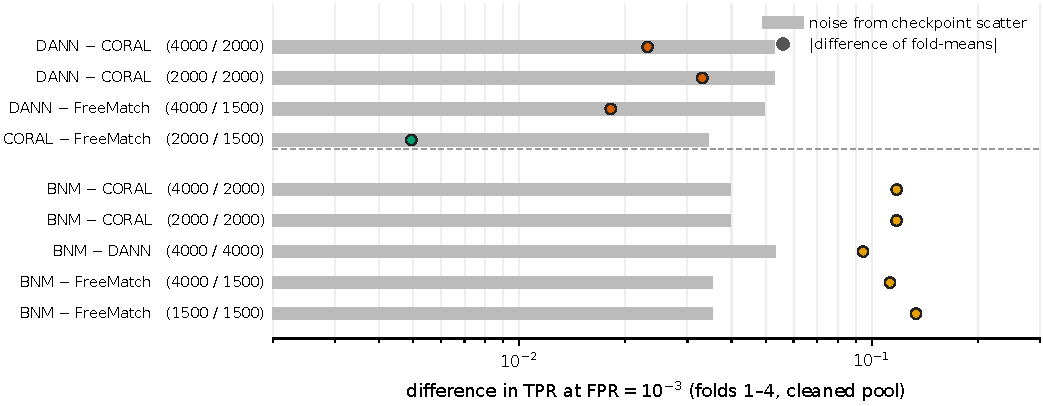
\includegraphics[width=\textwidth]{F5_resolution_v2.pdf}
\caption{\textbf{Differences between methods against checkpoint noise.} For each pair of
adaptation arms read at declared read-offs, the bar is the contribution of
checkpoint-to-checkpoint scatter to a difference of four-fold means, and the point is the
difference of the fold-means; log axis. As computed here, the gaps among CORAL, DANN and
FreeMatch (top) lie inside the noise and the gaps between BNM and each of them (bottom) lie
outside it. The bars assume
that the two arms' checkpoint noise is independent, which overstates it
(Section~\ref{sec:resolution}).}
\label{fig:resolution}
\end{figure}

\section{The frozen comparison: results, augmentation and precision}
\label{sec:augprec}

\subsection{The frozen comparison}
\label{sec:frozen-comparison}

Table~\ref{tab:frozen} gives the frozen comparison that Section~\ref{sec:results-frozen}
summarises. We report no frozen-against-unfrozen contrast except one.
Eight configuration fields separate the frozen and unfrozen CORAL runs: head learning rate,
weight decay, cached features against images, augmentation, precision, the weight schedule, the
weight, and target-covariance averaging. A difference between them would mix the encoder
setting with the protocol. The exception is FreeMatch, whose frozen and unfrozen runs share
every training setting except the encoder and the further steps of training
(Section~\ref{sec:results-frozen}).

% GENERATED FILE -- do not edit by hand.
% Rebuild:  python make_all.py (generator: make_main_tables_v2.py)
% Table 1 (rewrite v1): the frozen comparison at two decimals. Sources as T3_round1.tex.
\begin{table}[tbp]
\centering
\caption{\textbf{The frozen comparison.} Means over folds 0--4, the development fold included (with across-fold sd), of TPR at FPR${}=10^{-3}$, encoder frozen, 8000 steps, last checkpoint. Differences against Baseline A are paired by fold over the same five folds, with 95\% intervals from the class-conditional paired bootstrap ($B=1000$). DANN ran on the development fold only, with a different adapter and budget, and on the original test pool; every other row uses the cleaned pool.}
\label{tab:frozen}
\footnotesize
\setlength{\tabcolsep}{4pt}
\begin{tabular}{l>{\TRAG}p{3.6cm}rr}
\toprule
Method & Family & TPR@$10^{-3}$ & vs.\ Baseline A, 95\% CI \\
\midrule
Baseline A & source only & $0.20 \pm 0.04$ & --- \\
CORAL & marginal alignment (moment matching) & $0.22 \pm 0.03$ & $+0.02$ $[+0.0001, +0.05]$ \\
AdaMatch & self-training & $0.43 \pm 0.05$ & $+0.23$ $[+0.17, +0.28]$ \\
FreeMatch & self-training & $0.43 \pm 0.03$ & $+0.23$ $[+0.19, +0.30]$ \\
\midrule
DANN (fold 0) & marginal alignment (adversarial) & $0.19$ & --- \\
\bottomrule
\end{tabular}
\end{table}


\subsection{Augmentation and precision}
\label{sec:augprec-detail}

The arms of the frozen comparison were not trained under identical conditions. The
feature-space arms ran on cached features, without augmentation, in full precision; the
image-space arms ran with weak augmentation (Section~\ref{sec:sim-pipeline}) in mixed precision, because weak and strong views
are the mechanism of self-training. We measured that pair of variables on the frozen
source-only baseline on the development fold, where only the head's \augprecTrainableNs{}
parameters train.

We ran three of the four cells of the $2 \times 2$ (Table~\ref{tab:augprec2}). Cell~A, no
augmentation at full precision, is the configuration of the feature-space arms; cell~C, weak
augmentation at half precision, is that of the image-space arms; cell~B, weak augmentation at
full precision, sits between them. We did not run cell~D, no augmentation at half precision.
Cell~A reads \augprecCellA{} on this pool, one positive below the Baseline~A value of
\augprecBaselineFoldZero{}; the two matched at $\baseFoldZeroPrereg{}$ on the original pool. We
ran all three cells locally so that they share one venue; the same cell~C configuration on
Kaggle reads \augprecCellCKaggle{}, \augprecVenueLenses{} positives higher
(\augprecVenueDiff{}, interval \augprecVenueCI).

The total difference $C - A$ is \augprecTotal{}, 95\% interval \augprecTotalCI. Its upper bound
sits one positive (\augprecOnePos{} on 98) from zero. The path $A \to B \to C$ splits it into
an augmentation leg, $B - A$, of \augprecAug{} \augprecAugCI, and a precision leg, $C - B$, of
\augprecPrec{} \augprecPrecCI; neither leg's interval excludes zero. The legs sum to the total
only because the path is a chain, and without cell~D the interaction is not identified. The
augmentation leg has the larger point estimate, \augprecAugLenses{} positives against
\augprecPrecLenses{}, but with both intervals containing zero we do not name augmentation as
the cause. With so few trainable parameters, augmentation mostly injects noise into a fixed
feature space; with the encoder unfrozen it would normally help, so none of these values says
that augmentation is harmful.

% GENERATED FILE -- do not edit by hand.
% Rebuild:  python make_all.py (generator: make_appendix_relabel_v2.py)
% Relabelled copy of tables/A4_augprec.tex; tabular number tokens asserted identical, caption/notes token changes declared.
\begin{table}[htbp]
\centering
\caption{\textbf{Augmentation and precision in the frozen comparison, three cells of a $2\times2$.} Frozen encoder (Baseline A), development fold 0, 1921 trainable parameters, 98 test positives. Cell D was never run, so the interaction between the two factors is not identified. Differences are paired class-conditional bootstrap estimates (2000 replicates, 95\% percentile interval); the one-positive resolution is $1/98$. The two legs sum to the total exactly because $A\to B\to C$ is a chain, which is arithmetic and not evidence that the effects add.}
\label{tab:augprec2}
\footnotesize
\setlength{\tabcolsep}{4pt}
\begin{tabular}{lllrr}
\toprule
Cell & Augmentation & Precision & TPR@$10^{-3}$ & AUROC \\
\midrule
A & none & fp32 & $0.2347$ & $0.9440$ \\
B & weak & fp32 & $0.1735$ & $0.9226$ \\
C & weak & fp16 & $0.1531$ & $0.9256$ \\
D & none & fp16 & \emph{not run} & \emph{not run} \\
\bottomrule
\end{tabular}

\vspace{6pt}
\footnotesize
\setlength{\tabcolsep}{4pt}
\begin{tabular}{llrlr}
\toprule
Leg & Path & $\Delta$TPR@$10^{-3}$ & 95\% interval & Excludes 0 \\
\midrule
Augmentation (held at fp32) & $B-A$ & $-0.0612$ & $[-0.1327, +0.0000]$ & no \\
Precision (held at weak augmentation) & $C-B$ & $-0.0204$ & $[-0.0510, +0.0204]$ & no \\
Total & $C-A$ & $-0.0816$ & $[-0.1429, -0.0102]$ & yes \\
\bottomrule
\end{tabular}
\end{table}


\section{Reconstructing training state across a checkpoint restart}
\label{sec:appendix-restart}

The unfrozen FreeMatch arm continues from its frozen-comparison head. Those checkpoints store
four keys, \restartKeys{}, so the model survives and the training state around it does not.
Continuing from such a checkpoint restarts three things: the self-adaptive threshold state,
which re-initialises to $1/C$; the consistency weight's warm-up, which holds the consistency term at
zero for the first \restartMuZeroSteps{} steps of the \restartScheduleStepsNs{}-step schedule;
and AdamW's moment estimates. The fixes below implement the pre-registered intent that the
decision boundary and the threshold start consistent with each other. Every TPR value in this
appendix is on the original test pool, as each run scored it during training.

\paragraph{The evidence.} A \restartControlStepsNs{}-step frozen continuation of the
development-fold head, with none of this state rebuilt, ran \restartStart{} $\to$
\restartTrough{} at step \restartTroughStep{} $\to$ \restartEnd{} in TPR@$10^{-3}$, a maximum
drift of \restartMaxDrift{} (\restartMaxDriftPos{} positives against a one-positive resolution
of \restartOnePos{}), with the trough inside the window where the consistency term is held at zero.

\paragraph{The fixes.} \emph{Threshold state:} with the weights fixed, the moving average has
the pool mean as its fixed point, so we rebuilt it by averaging per-batch statistics over
\restartSatPasses{} weakly augmented passes of the \restartPool{}-image target pool
(\restartSatBatches{} batches). Driving the real update rule, momentum \restartMomentum{}, for
\restartEmaItersNs{} iterations agrees with this to \restartTauAgree{} on the global threshold and
\restartPbarAgree{} on the class marginal, against a tolerance of \restartSatTol{}.
\emph{Warm-up offset:} we resume the consistency-weight schedule at step \restartMuOffsetNs{}, so
the consistency term is at full weight from the first step. \emph{Moment warm-up:} AdamW runs
\restartAdamSteps{} steps under the corrected objective with the weights restored after every
step and the encoder frozen. A probe continues to step \restartAdamProbeEnd{}, over which the
bias-corrected second moment moved \restartAdamDebiased{} from step \restartAdamSteps{}, and
then rolls the optimiser state back to step \restartAdamSteps{}; it does not roll back the
threshold state, which the probe's forward passes keep updating, or the half-precision loss
scale. We call this reconstruction, not restoration: the original values were never stored.
The order is load the head, rebuild the threshold state, warm the moments, unfreeze, train.

\paragraph{The reconstructed control.} With the three fixes, the same frozen continuation
drifts at most \restartFixedMaxDrift{} from step 0 (\restartFixedMaxDriftPos{} positives). Over
its \restartFixedN{} later checkpoints its mean is \restartFixedMean{} (sd \restartFixedSD{}),
against \restartTailMean{} (sd \restartTailSD{}) over the last \restartTailN{} checkpoints of
the frozen run itself; we ran no test of their equality.

\paragraph{The step-0 gate.} Every fold is gated before training (Table~\ref{tab:restartgate2}).
We first required exact reproduction of TPR@$10^{-3}$. That held on the development fold and on
fold 1 and refused fold 2, whose step-0 value differed by one positive: scoring through the
encoder inside the training loop drifts slightly from the cached scoring path. We recalibrated
the rule before rerunning fold 2, to TPR within one positive together with an AUROC check at
$10^{-3}$, and folds 2--4 passed.

% GENERATED FILE -- do not edit by hand.
% Rebuild:  python make_all.py (generator: make_appendix_relabel_v2.py)
% Relabelled copy of tables/A5_gate.tex; tabular number tokens asserted identical, caption/notes token changes declared.
\begin{table}[t]
\centering
\caption{\textbf{The per-fold step-0 gate, as each run recorded it} (unfrozen FreeMatch). The gate re-scores the loaded head before any training and aborts the fold on a mismatch. Folds 0 and 1 ran under the original rule, exact reproduction of TPR@$10^{-3}$; fold 2 differed by exactly one positive, which that rule refuses, and folds 2--4 ran under the recalibrated rule. TPR differences are in positives; the AUROC half was added with the recalibration.}
\label{tab:restartgate2}
\footnotesize
\setlength{\tabcolsep}{4pt}
\begin{tabular}{llrr}
\toprule
Fold & Rule & $|\Delta\mathrm{TPR}|$ (positives) & $|\Delta\mathrm{AUROC}|$ \\
\midrule
0 (development) & TPR exact & 0 & --- \\
1 (confirmatory) & TPR exact & 0 & --- \\
2 (confirmatory) & TPR $\le$ 1 positive; AUROC $\le 10^{-3}$ & 1 & $3.7 \times 10^{-6}$ \\
3 (confirmatory) & TPR $\le$ 1 positive; AUROC $\le 10^{-3}$ & 0 & $9.5 \times 10^{-6}$ \\
4 (confirmatory) & TPR $\le$ 1 positive; AUROC $\le 10^{-3}$ & 0 & $1.4 \times 10^{-5}$ \\
\bottomrule
\end{tabular}
\end{table}


\section{The splits audit}
\label{sec:splitrules}

Our split-building script enforces nine rule groups before it writes the splits file, and any
failure aborts the build. The grouping and numbering are the script's own;
Section~\ref{sec:data} describes the independent check we ran afterwards and what it found.

\begin{table}[htbp]
\centering
\footnotesize
\setlength{\tabcolsep}{4pt}
\caption{\textbf{The split audit.} Enforced on the real data when the splits file is built;
all nine groups pass. ``Partition'' is the hash-partition index each unlabelled galaxy
carries, used here to keep the four negative roles disjoint.}
\label{tab:splitrules}
\begin{tabular}{rp{0.82\textwidth}}
\toprule
& Rule group \\
\midrule
1 & The simulated train and validation rows are disjoint, and no deflector is shared
between them; grouping by deflector identifier, not merely by image, prevents the
reused-host leak. \\
2 & Bare-deflector negatives are unique by object identifier, each drawn from the correct
side of the train/validation split, and none appears on both sides. \\
3 & Each source side is balanced 1:1, positives against negatives. \\
4 & Random negatives come from the partition reserved for their role: train, validation
and test each from their own. A foreign identifier maps to a sentinel rather than raising,
so a leak is flagged rather than crashing the audit. \\
5 & Every random-negative draw is mutually disjoint: train, validation, test and all five
target folds. Target negatives are disjoint from test negatives, target folds are
disjoint from one another (fresh per fold), and every
target draw comes from the target partition. \\
6 & For each fold, the test and target lens rows partition the 489 graded lenses
with no overlap and no remainder, and across the five folds each lens is tested exactly
once. \\
7 & Every fold's test positives contain both grades, so no fold is graded A-only or
B-only. \\
8 & Grade-X hard negatives appear in training only, and never in a validation, test or
target pool. \\
9 & No simulation deflector appears, by stored identifier, among the random-galaxy negatives
drawn for training, validation, test or any fold's target. The bare-deflector negatives are
simulation hosts by design, and the grade-X hard negatives are not part of this check.
Section~\ref{sec:data} gives the result of the same check by exact ID. \\
\bottomrule
\end{tabular}
\end{table}

\section{Results on the original test pool}
\label{app:prereg_pool}

Table~\ref{tab:prereg_pool6} gives the fold-means and the paired contrasts on the original test
pool (the pool as drawn and pre-registered, before the exclusion of
Section~\ref{sec:testpool}), on the cleaned pool of the main text, and on the cleaned pool without the \DTwoPositives{} test lenses that also appear as
training or validation negatives (``reduced''). On the original pool every arm's TPR is lower,
and no contrast of the main design changes whether its interval includes zero.

% GENERATED FILE -- do not edit by hand.
% Rebuild:  python make_all.py (generator: make_dilute10_tables.py)
% Paper v6: tables/A7_prereg_pool_v2.tex unchanged except 1 reference(s) to Table 2 (tab:contrasts2 -> tab:contrasts6) and its label (tab:prereg_pool2 -> tab:prereg_pool6).
\begin{table}[htbp]
\centering
\caption{Fold-mean TPR@$10^{-3}$ (folds 1--4) and the paired contrasts on the
original test pool (test negatives exactly as drawn), on the cleaned pool of the
main text, which excludes the 265 objects of
Section~\ref{sec:testpool}, and on that pool also without the 20 test lenses of Section~\ref{sec:testpool} (``reduced'').}
\label{tab:prereg_pool6}
\footnotesize
\setlength{\tabcolsep}{4pt}
\begin{tabular}{lrrrr}
\toprule
\multicolumn{5}{l}{\textit{(a) Fold-mean TPR@$10^{-3}$}} \\
Arm & Read at & Original & cleaned pool & reduced \\
\midrule
CORAL & 2000 & $0.4348$ & $0.5216$ & $0.5208$ \\
FreeMatch & 1500 & $0.4169$ & $0.5167$ & $0.5114$ \\
DANN & 4000 & $0.4167$ & $0.4985$ & $0.4997$ \\
DANN, sensitivity readout & 2000 & $0.4551$ & $0.5547$ & $0.5547$ \\
$\lambda=0$ unfrozen control & 4000 & $0.1355$ & $0.1842$ & $0.1852$ \\
BNM & 4000 & $0.3274$ & $0.4040$ & $0.4087$ \\
Baseline A (frozen) & 8000 & $0.1714$ & $0.1842$ & $0.1742$ \\
\bottomrule
\end{tabular}

\vspace{6pt}
\footnotesize
\setlength{\tabcolsep}{4pt}
\begin{tabular}{>{\TRAG}p{3.0cm}lllc}
\toprule
\multicolumn{5}{l}{\textit{(b) Paired contrasts, $\Delta$ TPR@$10^{-3}$ and 95\% CI}} \\
Contrast & Steps & Original & cleaned pool & Zero-inclusion \\
\midrule
$\lambda=0$ $-$ Baseline A & 4000 / 8000 & $-0.0360$ $[-0.1249, +0.0530]$ & $0.0000$$^{\dagger}$ $[-0.0890, +0.0889]$ & same \\
DANN $-$ $\lambda=0$ & 4000 / 4000 & $+0.2812$ $[+0.0595, +0.5029]$ & $+0.3144$ $[+0.0565, +0.5722]$ & same \\
CORAL $-$ $\lambda=0$ & 2000 / 2000 & $+0.2607$ $[+0.0976, +0.4238]$ & $+0.3068$ $[+0.1834, +0.4301]$ & same \\
FreeMatch $-$ $\lambda=0$ & 1500 / 1500 & $+0.2712$ $[+0.1649, +0.3776]$ & $+0.3223$ $[+0.1984, +0.4463]$ & same \\
BNM $-$ $\lambda=0$ & 4000 / 4000 & $+0.1919$ $[+0.1278, +0.2561]$ & $+0.2199$ $[+0.1383, +0.3014]$ & same \\
CORAL $-$ $\lambda=0$ (at 4000) & 2000 / 4000 & $+0.2993$ $[+0.1386, +0.4600]$ & $+0.3375$ $[+0.1889, +0.4860]$ & same \\
FreeMatch $-$ $\lambda=0$ (at 4000) & 1500 / 4000 & $+0.2815$ $[+0.1858, +0.3771]$ & $+0.3325$ $[+0.2272, +0.4378]$ & same \\
BNM $-$ CORAL & 2000 / 2000 & $-0.0920$ $[-0.1680, -0.0160]$ & $-0.1176$ $[-0.1772, -0.0580]$ & same \\
BNM $-$ DANN & 4000 / 4000 & $-0.0893$ $[-0.2887, +0.1101]$ & $-0.0945$ $[-0.3104, +0.1214]$ & same \\
BNM $-$ FreeMatch & 1500 / 1500 & $-0.1180$ $[-0.2578, +0.0219]$ & $-0.1334$ $[-0.2986, +0.0319]$ & same \\
DANN $-$ CORAL & 4000 / 2000 & $-0.0180$ $[-0.1781, +0.1420]$ & $-0.0231$ $[-0.2227, +0.1765]$ & same \\
DANN $-$ FreeMatch & 4000 / 1500 & $-0.0002$ $[-0.1656, +0.1652]$ & $-0.0182$ $[-0.2092, +0.1729]$ & same \\
DANN $-$ CORAL (both at 2000) & 2000 / 2000 & $+0.0203$ $[-0.0772, +0.1179]$ & $+0.0331$ $[-0.0711, +0.1372]$ & same \\
\midrule
FreeMatch unfrozen $-$ frozen$^{\ast}$ & 1500 / 8000 & $+0.0793$ $[+0.0075, +0.1690]$ & $+0.1049$ $[+0.0256, +0.1687]$ & same \\
\bottomrule
\end{tabular}

\vspace{2pt}
\footnotesize Intervals as in Table~\ref{tab:contrasts6}: paired $t$, df $=3$;
$^{\ast}$fold-aware paired bootstrap, $B=5000$. $^{\dagger}$$-0.00003$ before rounding.
\end{table}


\section{The bright-only test pool}
\label{app:bright}

The benchmark's non-lens sample is limited at $I_E < 22.5$, and \FracFaintTest{}\% of our
cleaned test negatives are fainter than that in VIS PSF magnitude. We therefore repeated the
main readouts on the $\rvBrightN{}$ cleaned negatives brighter than 22.5, with the positives
unchanged (Table~\ref{tab:bright}). Every contrast in Table~\ref{tab:bright} keeps its zero-inclusion. TPR falls slightly
for every arm, and BNM's benchmark ratio falls the most, from $\rvBnmDOneRatio{}$ to
$\rvBnmBrightRatio{}$. This analysis was done after the results were known.

% GENERATED FILE -- do not edit by hand.
% Rebuild:  python make_all.py (generator: make_appendix_tables_v2.py)
% Appendix H (rewrite v1): audit/review_r1b/out/L2_bright_pool.json.
\begin{table}[htbp]
\centering
\caption{\textbf{The bright-only test pool.} The cleaned test negatives with VIS PSF magnitude $\le 22.5$ ($14\,950$ of $26\,134$; the magnitude limit of Section~\ref{sec:splits}); positives unchanged. (a) TPR at FPR${}=10^{-3}$, folds 1--4. (b) Paired contrasts, paired $t$, df${}=3$. (c) Completeness at 24\% purity and its ratio to 0.50; n/a where any fold is undefined.}
\label{tab:bright}
\footnotesize
\setlength{\tabcolsep}{4pt}
\begin{tabular}{lrrrrrrrr}
\toprule
\multicolumn{9}{l}{\textit{(a) TPR@$10^{-3}$}} \\
Readout & f1 & f2 & f3 & f4 & mean & sd & cleaned pool & change \\
\midrule
Baseline A (8000) & $0.1429$ & $0.2143$ & $0.1633$ & $0.2062$ & $0.1816$ & $0.0342$ & $0.1842$ & $-0.0026$ \\
$\lambda=0$ (4000) & $0.2245$ & $0.1429$ & $0.1122$ & $0.1031$ & $0.1457$ & $0.0552$ & $0.1842$ & $-0.0385$ \\
BNM (4000) & $0.3673$ & $0.4388$ & $0.3367$ & $0.3814$ & $0.3811$ & $0.0428$ & $0.4040$ & $-0.0230$ \\
FreeMatch (1500) & $0.4796$ & $0.5510$ & $0.3776$ & $0.5361$ & $0.4861$ & $0.0786$ & $0.5167$ & $-0.0306$ \\
DANN (4000) & $0.5000$ & $0.7041$ & $0.2857$ & $0.3608$ & $0.4627$ & $0.1838$ & $0.4985$ & $-0.0359$ \\
DANN (2000, sens.) & $0.5408$ & $0.7041$ & $0.4694$ & $0.4227$ & $0.5342$ & $0.1232$ & $0.5547$ & $-0.0205$ \\
CORAL (2000) & $0.4694$ & $0.6122$ & $0.5000$ & $0.4742$ & $0.5140$ & $0.0669$ & $0.5216$ & $-0.0077$ \\
\bottomrule
\end{tabular}

\vspace{6pt}
\footnotesize
\setlength{\tabcolsep}{4pt}
\begin{tabular}{llrrrc}
\toprule
\multicolumn{6}{l}{\textit{(b) Paired contrasts, $\Delta$ and 95\% CI}} \\
Contrast & Steps & bright pool & 95\% CI & cleaned pool & 0 excluded in both \\
\midrule
DANN $-$ $\lambda=0$ & 4000 / 4000 & $+0.3170$ & $[+0.0484, +0.5856]$ & $+0.3144$ & yes \\
CORAL $-$ $\lambda=0$ & 2000 / 4000 & $+0.3683$ & $[+0.2206, +0.5160]$ & $+0.3375$ & yes \\
CORAL $-$ $\lambda=0$ & 2000 / 2000 & $+0.3399$ & $[+0.1893, +0.4906]$ & $+0.3068$ & yes \\
FreeMatch $-$ $\lambda=0$ & 1500 / 4000 & $+0.3404$ & $[+0.1920, +0.4888]$ & $+0.3325$ & yes \\
FreeMatch $-$ $\lambda=0$ & 1500 / 1500 & $+0.3276$ & $[+0.1768, +0.4784]$ & $+0.3223$ & yes \\
BNM $-$ $\lambda=0$ & 4000 / 4000 & $+0.2354$ & $[+0.1260, +0.3448]$ & $+0.2199$ & yes \\
BNM $-$ CORAL & 4000 / 2000 & $-0.1329$ & $[-0.1987, -0.0671]$ & $-0.1176$ & yes \\
BNM $-$ CORAL & 2000 / 2000 & $-0.1329$ & $[-0.1870, -0.0788]$ & $-0.1176$ & yes \\
\bottomrule
\end{tabular}

\vspace{6pt}
\footnotesize
\setlength{\tabcolsep}{4pt}
\begin{tabular}{lrrrrrrr}
\toprule
\multicolumn{8}{l}{\textit{(c) Completeness at 24\% purity}} \\
Readout & f1 & f2 & f3 & f4 & mean & ratio & ratio, cleaned pool \\
\midrule
Baseline A (8000) & $0.1224$ & $0.0714$ & $0.1020$ & $0.0928$ & $0.0972$ & $0.1944$ & $0.1841$ \\
$\lambda=0$ (4000) & $0.0714$ & \emph{n/a} & \emph{n/a} & $0.0103$ & \emph{n/a} & \emph{n/a} & \emph{n/a} \\
BNM (4000) & $0.1939$ & $0.2857$ & $0.2551$ & $0.3608$ & $0.2739$ & $0.5478$ & $0.7110$ \\
FreeMatch (1500) & $0.4592$ & $0.5510$ & $0.3265$ & $0.5258$ & $0.4656$ & $0.9313$ & $0.9670$ \\
DANN (4000) & $0.4286$ & $0.7143$ & $0.2245$ & $0.3093$ & $0.4192$ & $0.8383$ & $0.9100$ \\
DANN (2000, sens.) & $0.5408$ & $0.7041$ & $0.3878$ & $0.4124$ & $0.5113$ & $1.0225$ & $1.0582$ \\
CORAL (2000) & $0.3571$ & $0.6122$ & $0.4796$ & $0.4330$ & $0.4705$ & $0.9410$ & $0.9922$ \\
\bottomrule
\end{tabular}
\end{table}


\section{Recall by lens property, and the highest-scoring negatives}
\label{app:breakdowns}

Table~\ref{tab:gradeperfold} gives the per-fold counts behind Table~\ref{tab:graderecall}.
Table~\ref{tab:recallprop} bins the confirmatory test lenses by expert score, modelled Einstein
radius, lensed-source magnitude and lensed-source signal-to-noise ratio, the per-lens columns
stored with the Discovery Engine catalogue; the last three exist for $\rvThetaN{}$ of the
$\rvConfTestN{}$ lenses. Table~\ref{tab:topneg} lists the 25 cleaned-pool negatives placed above
threshold most often across the seven readouts and four folds. All of this is descriptive and
was done after the results were known.

% GENERATED FILE -- do not edit by hand.
% Rebuild:  python make_all.py (generator: make_appendix_tables_v2.py)
% Appendix I (rewrite v1): audit/review_r1/out/A3_recall_by_grade.json.
\begin{table}[htbp]
\centering
\caption{\textbf{Recall by grade, per fold}, at each fold's FPR${}=10^{-3}$ threshold on the cleaned pool: recovered/total. Sums and intervals: Table~\ref{tab:graderecall}.}
\label{tab:gradeperfold}
\footnotesize
\setlength{\tabcolsep}{4pt}
\begin{tabular}{lrrrrrrrr}
\toprule
 & \multicolumn{4}{c}{grade A} & \multicolumn{4}{c}{grade B} \\
\cmidrule(lr){2-5}\cmidrule(lr){6-9}
Readout & f1 & f2 & f3 & f4 & f1 & f2 & f3 & f4 \\
\midrule
Baseline A (8000) & 10/49 & 14/49 & 12/49 & 16/49 & 4/49 & 7/49 & 5/49 & 4/48 \\
$\lambda=0$ (4000) & 16/49 & 13/49 & 11/49 & 15/49 & 6/49 & 4/49 & 3/49 & 4/48 \\
BNM (4000) & 27/49 & 32/49 & 28/49 & 29/49 & 12/49 & 13/49 & 9/49 & 8/48 \\
FreeMatch (1500) & 32/49 & 34/49 & 32/49 & 38/49 & 17/49 & 24/49 & 10/49 & 15/48 \\
DANN (4000) & 32/49 & 43/49 & 22/49 & 32/49 & 21/49 & 27/49 & 9/49 & 9/48 \\
DANN (2000, sens.) & 35/49 & 42/49 & 35/49 & 32/49 & 21/49 & 27/49 & 14/49 & 11/48 \\
CORAL (2000) & 32/49 & 38/49 & 35/49 & 34/49 & 14/49 & 24/49 & 14/49 & 13/48 \\
\bottomrule
\end{tabular}
\end{table}


% GENERATED FILE -- do not edit by hand.
% Rebuild:  python make_all.py (generator: make_appendix_tables_v2.py)
% Appendix I (rewrite v1): audit/review_r1/out/A3_recall_by_property.json.
\begin{table}[htbp]
\centering
\caption{\textbf{Recall by lens property}, folds 1--4, cleaned pool. Bins are tertiles of the confirmatory test lenses that have a value (edges given); cells are recovered/total and rate. Einstein radius and arc values come from the lens-modelling tables stored with the Discovery Engine catalogue and exist for a subset of lenses; stored values of exactly 0 and one arc magnitude above 30 are kept as stored.}
\label{tab:recallprop}
\scriptsize
\begin{tabular}{lrrr}
\toprule
\multicolumn{4}{l}{\textit{Expert score}: 391 of 391 lenses; edges 1.50, 1.76, 2.24, 3.16} \\
\midrule
Readout & low & middle & high \\
Baseline A (8000) & 10/131 ($0.08$) & 22/130 ($0.17$) & 40/130 ($0.31$) \\
$\lambda=0$ (4000) & 10/131 ($0.08$) & 19/130 ($0.15$) & 43/130 ($0.33$) \\
BNM (4000) & 23/131 ($0.18$) & 51/130 ($0.39$) & 84/130 ($0.65$) \\
FreeMatch (1500) & 36/131 ($0.27$) & 67/130 ($0.52$) & 99/130 ($0.76$) \\
DANN (4000) & 36/131 ($0.27$) & 68/130 ($0.52$) & 91/130 ($0.70$) \\
DANN (2000, sens.) & 39/131 ($0.30$) & 76/130 ($0.58$) & 102/130 ($0.78$) \\
CORAL (2000) & 36/131 ($0.27$) & 67/130 ($0.52$) & 101/130 ($0.78$) \\
\midrule
\multicolumn{4}{l}{\textit{Einstein radius ($''$)}: 245 of 391 lenses; edges 0.00, 0.71, 1.01, 4.31} \\
\midrule
Readout & low & middle & high \\
Baseline A (8000) & 8/82 ($0.10$) & 22/81 ($0.27$) & 24/82 ($0.29$) \\
$\lambda=0$ (4000) & 9/82 ($0.11$) & 28/81 ($0.35$) & 27/82 ($0.33$) \\
BNM (4000) & 25/82 ($0.30$) & 47/81 ($0.58$) & 48/82 ($0.59$) \\
FreeMatch (1500) & 39/82 ($0.48$) & 53/81 ($0.65$) & 56/82 ($0.68$) \\
DANN (4000) & 38/82 ($0.46$) & 59/81 ($0.73$) & 48/82 ($0.59$) \\
DANN (2000, sens.) & 48/82 ($0.59$) & 57/81 ($0.70$) & 57/82 ($0.70$) \\
CORAL (2000) & 46/82 ($0.56$) & 56/81 ($0.69$) & 55/82 ($0.67$) \\
\midrule
\multicolumn{4}{l}{\textit{Arc magnitude (VIS, AB)}: 245 of 391 lenses; edges 18.11, 21.95, 22.57, 41.08} \\
\midrule
Readout & low & middle & high \\
Baseline A (8000) & 22/82 ($0.27$) & 15/81 ($0.19$) & 17/82 ($0.21$) \\
$\lambda=0$ (4000) & 25/82 ($0.30$) & 20/81 ($0.25$) & 19/82 ($0.23$) \\
BNM (4000) & 44/82 ($0.54$) & 37/81 ($0.46$) & 39/82 ($0.48$) \\
FreeMatch (1500) & 48/82 ($0.59$) & 47/81 ($0.58$) & 53/82 ($0.65$) \\
DANN (4000) & 50/82 ($0.61$) & 47/81 ($0.58$) & 48/82 ($0.59$) \\
DANN (2000, sens.) & 52/82 ($0.63$) & 56/81 ($0.69$) & 54/82 ($0.66$) \\
CORAL (2000) & 54/82 ($0.66$) & 48/81 ($0.59$) & 55/82 ($0.67$) \\
\midrule
\multicolumn{4}{l}{\textit{Arc S/N}: 245 of 391 lenses; edges 0.00, 8.67, 13.83, 121.36} \\
\midrule
Readout & low & middle & high \\
Baseline A (8000) & 24/82 ($0.29$) & 18/81 ($0.22$) & 12/82 ($0.15$) \\
$\lambda=0$ (4000) & 26/82 ($0.32$) & 23/81 ($0.28$) & 15/82 ($0.18$) \\
BNM (4000) & 43/82 ($0.52$) & 42/81 ($0.52$) & 35/82 ($0.43$) \\
FreeMatch (1500) & 54/82 ($0.66$) & 51/81 ($0.63$) & 43/82 ($0.52$) \\
DANN (4000) & 50/82 ($0.61$) & 46/81 ($0.57$) & 49/82 ($0.60$) \\
DANN (2000, sens.) & 55/82 ($0.67$) & 57/81 ($0.70$) & 50/82 ($0.61$) \\
CORAL (2000) & 58/82 ($0.71$) & 50/81 ($0.62$) & 49/82 ($0.60$) \\
\bottomrule
\end{tabular}
\end{table}


% GENERATED FILE -- do not edit by hand.
% Rebuild:  python make_all.py (generator: make_appendix_tables_v2.py)
% Appendix I (rewrite v1): audit/review_r1/out/top_negatives.csv, counts re-derived from A2_top_negatives.json.
\begin{table}[htbp]
\centering
\caption{\textbf{The test negatives most often above threshold.} The 25 cleaned-pool negatives placed above the FPR${}=10^{-3}$ threshold in the most of the 28 readout-by-fold cells (seven readouts, four folds); position and VIS PSF magnitude from the MER catalogue; best rank among the negatives of any cell; grade where the object is in the Discovery Engine catalogue. We make no claim about their nature.}
\label{tab:topneg}
\footnotesize
\setlength{\tabcolsep}{4pt}
\begin{tabular}{rrrrrrc}
\toprule
Euclid ID & RA ($^\circ$) & Dec ($^\circ$) & VIS mag & cells & best rank & grade \\
\midrule
$-517924132270604029$ & 51.79241 & $-27.06040$ & 20.19 & 26 & 2 & --- \\
$-643651713458899270$ & 64.36517 & $-45.88993$ & 22.18 & 24 & 1 & --- \\
$-516036689288795768$ & 51.60367 & $-28.87958$ & 20.43 & 23 & 1 & --- \\
$-614740525474565457$ & 61.47405 & $-47.45655$ & 21.00 & 21 & 1 & C \\
$2721660958665742075$ & 272.16610 & $+66.57421$ & 22.61 & 20 & 5 & C \\
$2720771193650236654$ & 272.07712 & $+65.02367$ & 22.01 & 18 & 3 & --- \\
$2732051754679859830$ & 273.20518 & $+67.98598$ & 20.06 & 18 & 3 & --- \\
$-577967901484934075$ & 57.79679 & $-48.49341$ & 20.92 & 17 & 3 & --- \\
$-572039058485602501$ & 57.20391 & $-48.56025$ & 20.63 & 16 & 2 & --- \\
$-604699501484627657$ & 60.46995 & $-48.46277$ & 22.75 & 16 & 3 & --- \\
$-623737529459802118$ & 62.37375 & $-45.98021$ & 22.17 & 15 & 1 & --- \\
$2740322988653754338$ & 274.03230 & $+65.37543$ & 21.95 & 13 & 1 & --- \\
$-534584955272049779$ & 53.45850 & $-27.20498$ & 22.90 & 12 & 1 & --- \\
$-618203476468103201$ & 61.82035 & $-46.81032$ & 22.83 & 12 & 2 & --- \\
$2674724083652311112$ & 267.47241 & $+65.23111$ & 21.65 & 11 & 1 & C \\
$2726502651673983321$ & 272.65027 & $+67.39833$ & 22.31 & 11 & 1 & --- \\
$-645120138467379824$ & 64.51201 & $-46.73798$ & 21.72 & 11 & 2 & --- \\
$-650102945492303222$ & 65.01029 & $-49.23032$ & 22.08 & 11 & 4 & --- \\
$2736776880686750699$ & 273.67769 & $+68.67507$ & 22.93 & 11 & 5 & --- \\
$-652726602487221405$ & 65.27266 & $-48.72214$ & 22.79 & 10 & 3 & C \\
$-610649149472019714$ & 61.06491 & $-47.20197$ & 22.08 & 10 & 4 & --- \\
$-512397515272617657$ & 51.23975 & $-27.26177$ & 22.52 & 10 & 13 & --- \\
$-627788292494637657$ & 62.77883 & $-49.46377$ & 22.80 & 9 & 2 & --- \\
$2691532629662288078$ & 269.15326 & $+66.22881$ & 21.66 & 9 & 10 & C \\
$-626297517475989366$ & 62.62975 & $-47.59894$ & 22.47 & 8 & 2 & --- \\
\bottomrule
\end{tabular}
\end{table}


\section{Reproducibility and software}
\label{app:repro}

\paragraph{Encoder.} We load the encoder through \texttt{timm} from the Hugging Face hub by the
checkpoint string \texttt{hf\_hub:\allowbreak mwalmsley/\allowbreak zoobot-\allowbreak
encoder-\allowbreak greyscale-\allowbreak convnext\_nano}. The Zoobot package itself is not
installed and its version is not recorded; v2.0.1 is the release in which Zoobot's
documentation lists the greyscale encoders as added. The greyscale checkpoint has a
single-channel stem, so the model must be built with one input channel. Our unfrozen setting
trains timm \texttt{stages[3]}, \texttt{stages[2]} and \texttt{stages[1]}, the encoder's own
fine-tuning convention for $n_{\mathrm{blocks}} = 3$; the final layer normalisation is never
trained; the benchmark states only that it fine-tunes the last three
blocks~\citep{lines2025simstosky}.

\paragraph{Library versions.} We did not record the \texttt{timm} version used in training or
pin it in a requirements file. The notebook for the unfrozen FreeMatch arm installs
\texttt{timm} 1.0.26, but its outputs do not record the installed version, and the notebooks
for the other unfrozen arms install none, so they used the hosted environment's version; the
arms may therefore have run under different \texttt{timm} versions. Comments in our code name
1.0.26 and 1.0.28 as checked, and the per-stage parameter counts are a regression test, so a
release that renumbered the stages would fail a test. We installed GalSim unpinned in the WSL2
conda environment used for simulation and did not record its version, so the catalogue's default selection cannot be tied to
a known release. Our input stretch reproduces the \texttt{fits\_to\_jpg\_like\_scaling}
function of the \texttt{galaxy-datasets} package from its source code; we did not record the
package version or commit.

\paragraph{Compute venue and precision.} Every unfrozen arm trained in \venueTrainPrecision{}
and was scored in \venueEvalPrecision{}. The \venueGpuArms{} runs record a \venueGpu{}; the
FreeMatch runs record only a CUDA device, but their paths place them on Kaggle, and the
notebook settings we ship (\texttt{KAGGLE\_FREEMATCH\_PERFOLD\_CELLS.md}) specify a T4. We
measured the effect
of the venue once, on the frozen baseline with weak augmentation at half precision: the same
configuration scored \augprecCellC{} locally and \augprecCellCKaggle{} on Kaggle, a difference
of \augprecVenueDiff{} with interval \augprecVenueCI{} (Appendix~\ref{sec:augprec}). A second
check did not reproduce a venue effect: the same unfrozen CORAL weights scored in two separately
stored scorings gave identical TPR@$10^{-3}$ at all \venueCoralCheckpoints{} shared checkpoints
and AUROC agreeing to \venueCoralMaxAuroc{}.

\paragraph{The 1:10 runs.} The diluted DANN, BNM and unfrozen CORAL runs record a \venueGpu{};
the FreeMatch runs, frozen and unfrozen, record only a CUDA device; and the CORAL frozen stage
ran in full precision on CPU. Before FreeMatch's unfrozen runs, the pre-run check that part 3 of
the pre-registration requires reproduced the pattern of FreeMatch's early skipped updates in
its original mode, but not their exact count; we judged the match sufficient and proceeded,
since the rule does not say how closely the known-null must match. Before computing anything new,
the analysis reproduced this paper's balanced per-fold TPRs and its \dlReproNWord{} contrasts
against the control exactly, at four decimals.

\paragraph{Skipped updates.} In half precision the gradient scaler skips any step whose
gradients overflow. On folds 1--4 the balanced runs skipped \skipLamList{} steps (the control),
\skipDannList{} (DANN) and \skipCoralList{} (CORAL), and FreeMatch \skipFmEach{} on every fold;
the BNM runs did not record skips. Table~\ref{tab:dl-bookkeeping} gives the 1:10 runs'.

\paragraph{Infrastructure failures.} Three failures cost us time. Continuing training from a
weights-only checkpoint silently reset the training state; Appendix~\ref{sec:appendix-restart}
gives the cost and the repair. A gradient-norm measurement taken on CPU in fp32 moved by
$+\rvGradShiftPct{}$\% when re-measured on a T4 in fp16, enough to shift the weight grid derived
from it, so we re-derived the grid on the training hardware. An audit that found no
hard-coded write paths in our scripts was accurate when made, but a script written after it
wrote to one; we found it later and gave it an output flag and an overwrite guard.

\paragraph{Hash enrolment.} Two mechanisms implement our hash protection: discovery of every
file whose digest our run logs record (in the release, the digests in
\texttt{public\_inputs/\allowbreak record\_extract.json}), and a separate inventory that the
analysis scripts verify at
start and end. The checkpoint-window declaration of Appendix~\ref{sec:failed} is hashed but was
never enrolled in that inventory, so it is neither re-checked automatically nor read-only.
Its digest currently matches the file on disk, and Table~\ref{tab:hashes6} re-derives it at build
time and marks it as the one uncovered row. We did not enrol it after the fact, because that
would date its protection to the writing of this paper. The measuring run behind one hashed
gradient-norm grid was never downloaded, and the per-checkpoint files of two unfrozen
development runs on fold 0 were lost (Section~\ref{sec:negative}).

\paragraph{Script provenance.} The loss module that our four $\lambda = 0$ confirmatory folds ran
had since been overwritten in our working copy. We recovered it from the archived training
bundle, and its digest matches the one those runs recorded. Through line 1440 it is identical to
the version our DANN folds ran; the remainder is a BNM section that the $\lambda = 0$ training
path does not import, as the pre-registration's own audit, recovered with its recorded digest,
also documents. Four script versions used only by fold-0 development runs remain unrecovered;
they affect development-fold values only. The version of the unfrozen FreeMatch runner that
ran our balanced FreeMatch fold 1 is also unrecovered: its run record lacks \fmFoldOneMissingWord{} keys that
today's runner always writes and records the exact step-zero tolerance that preceded our gate
change (Appendix~\ref{sec:appendix-restart}), so the released runner is a later version.
For \dlLostArmsWord{} of the 1:10 arms (DANN, BNM and the CORAL and FreeMatch frozen
stages), the exact versions of \dlLostFilesWord{} helper scripts that ran
(\texttt{dilute10\_common.py}, \texttt{dilute10\_batch\_log.py} and the arm's wrapper) are lost;
the release has their later versions. Their recorded digests are in the run files. For
Baseline A, FreeMatch and CORAL's balanced frozen stage, the runs recorded no per-module digests,
and BNM's balanced runs recorded only the files its pre-registration hashes.

\paragraph{Where things are.} The contrast set and its registration marks are
\texttt{CONTRAST\_ROWS} and \texttt{CONTRAST\_PREREG} in \texttt{paper/scripts/\_common.py};
the four registered contrasts are in \texttt{runs/lambda0\_r6\_prereg.json}; the test-pool
exclusion rule is \texttt{audit/decontam/rule.json}; and the post hoc analyses of
Sections~\ref{sec:resolution}, \ref{sec:findmiss} and Appendices~\ref{app:bright}
and~\ref{app:breakdowns} are in \texttt{audit/review\_r1/}, \texttt{audit/review\_r1b/} and
\texttt{audit/rewrite\_v5/}; the
scripts that generate the tables, figures and number macros are in \texttt{paper/scripts/}.
The 1:10 experiment's contrasts and their mark are \texttt{DILUTE10\_CONTRASTS} and
\texttt{DILUTE10\_PREREG} in \texttt{paper/scripts/\_dilute10.py}; its three-part
pre-registration is
\texttt{runs/\allowbreak dilute10\_prereg\_\allowbreak part\{1,2,3\}.json}, its pool
\texttt{data/\allowbreak splits/\allowbreak dilute10\_pool.json}, its analysis
\texttt{runs/\allowbreak dilute10\_analysis/}, the frozen-stage head norms
\texttt{runs/\allowbreak dilute10\_head\_norms/}, and the memorisation diagnostic
\texttt{runs/\allowbreak dann\_lambda0\_holdout\_gap/}. The three files from the archived
training bundle, the loss module of the $\lambda = 0$ confirmatory folds, the
pre-registration's audit and the pre-registration itself, are
\texttt{evidence/\allowbreak kaggle\_bundle\_v14/\allowbreak da\_losses.py},
\texttt{evidence/\allowbreak kaggle\_bundle\_v14/\allowbreak lambda0\_r6\_audit.json} and
\texttt{evidence/\allowbreak kaggle\_bundle\_v14/\allowbreak lambda0\_r6\_prereg.json}.

\section{The 1:10 diluted-target experiment}
\label{app:dilute10}

This appendix gives the values behind Section~\ref{sec:results-dilute} at four decimals, and the
run facts the text cites. Every value comes from the experiment's analysis file or from the run
records named in Appendix~\ref{app:repro}; the methods are in Section~\ref{sec:dilute-methods}
and the pre-registration in Appendix~\ref{sec:prereg-dilute}.

\paragraph{Per-fold values and the ten intervals.} Table~\ref{tab:dl-perfold} gives every arm's
diluted values per fold for the four metrics of Appendix~\ref{app:perfold}, and
Table~\ref{tab:dl-contrasts4} the \dlNtWord{} paired $t$-intervals: the \dlNtG{} forms of $G$ and
the \dlNtD{} of $D$. The matched-step forms of $G$ give the same branches as the primary forms.

% GENERATED FILE -- do not edit by hand.
% Rebuild:  python make_all.py (generator: make_dilute10_tables.py)
% Appendix K: per-fold diluted values. runs/dilute10_analysis/results.json per_arm.
\begin{table}[htbp]
\centering
\caption{\textbf{Per-fold values of the diluted runs}, cleaned pool, at each arm's read-off step, with the fold-mean and sample sd. Completeness at 24\% purity and purity at 50\% completeness use the prevalence correction of Equation~\eqref{eq:purity}.}
\label{tab:dl-perfold}
\footnotesize
\setlength{\tabcolsep}{4pt}
\begin{tabular}{llrrrrrrr}
\toprule
Metric & Arm & Step & fold 1 & fold 2 & fold 3 & fold 4 & mean & sd \\
\midrule
TPR@$10^{-3}$ & DANN & 4000 & $0.5306$ & $0.5204$ & $0.5102$ & $0.5155$ & $0.5192$ & $0.0087$ \\
 & BNM & 4000 & $0.3980$ & $0.5408$ & $0.2857$ & $0.2887$ & $0.3783$ & $0.1203$ \\
 & CORAL & 2000 & $0.2449$ & $0.2041$ & $0.1531$ & $0.1753$ & $0.1943$ & $0.0397$ \\
 & FreeMatch & 1500 & $0.2959$ & $0.6327$ & $0.3469$ & $0.4742$ & $0.4374$ & $0.1502$ \\
\midrule
AUROC & DANN & 4000 & $0.9510$ & $0.8971$ & $0.8808$ & $0.7972$ & $0.8815$ & $0.0637$ \\
 & BNM & 4000 & $0.9445$ & $0.9804$ & $0.9218$ & $0.9096$ & $0.9391$ & $0.0311$ \\
 & CORAL & 2000 & $0.7813$ & $0.8089$ & $0.7990$ & $0.7610$ & $0.7876$ & $0.0211$ \\
 & FreeMatch & 1500 & $0.9660$ & $0.9874$ & $0.9731$ & $0.9781$ & $0.9762$ & $0.0090$ \\
\midrule
completeness at 24\% purity & DANN & 4000 & $0.5102$ & $0.5204$ & $0.4490$ & $0.4639$ & $0.4859$ & $0.0348$ \\
 & BNM & 4000 & $0.3163$ & $0.5204$ & $0.2449$ & $0.1134$ & $0.2988$ & $0.1700$ \\
 & CORAL & 2000 & $0.0408$ & $0.1020$ & $0.0408$ & $0.0619$ & $0.0614$ & $0.0289$ \\
 & FreeMatch & 1500 & $0.1735$ & $0.6327$ & $0.2551$ & $0.4227$ & $0.3710$ & $0.2030$ \\
\midrule
purity at 50\% completeness & DANN & 4000 & $0.2979$ & $0.2382$ & $0.1984$ & $0.1889$ & $0.2308$ & $0.0495$ \\
 & BNM & 4000 & $0.0915$ & $0.2707$ & $0.0571$ & $0.0179$ & $0.1093$ & $0.1117$ \\
 & CORAL & 2000 & $0.0194$ & $0.0147$ & $0.0072$ & $0.0072$ & $0.0121$ & $0.0060$ \\
 & FreeMatch & 1500 & $0.0991$ & $0.3726$ & $0.0803$ & $0.1776$ & $0.1824$ & $0.1336$ \\
\bottomrule
\end{tabular}
\end{table}


% GENERATED FILE -- do not edit by hand.
% Rebuild:  python make_all.py (generator: make_dilute10_tables.py)
% Appendix K: the 10 t-intervals. runs/dilute10_analysis/results.json G and D.
\begin{table}[htbp]
\centering
\caption{\textbf{The ten paired $t$-intervals of the 1:10 experiment} at four decimals, folds 1--4, cleaned pool (df${}=3$). $G$ is diluted $-$ $\lambda=0$; its primary form reads the control at 4000 and decides the branch, and its matched-step form, a pre-declared sensitivity readout, reads the control at the arm's own step. $D$ is balanced $-$ diluted at the same read-off; it carries no verdict and includes the noise of a changed batch order. No multiplicity correction. $^{*}$Interval excludes zero.}
\label{tab:dl-contrasts4}
\footnotesize
\setlength{\tabcolsep}{4pt}
\begin{tabular}{llrlcl}
\toprule
Contrast & Steps & $\Delta$ TPR@$10^{-3}$ & 95\% CI & Signs & Role \\
\midrule
\multicolumn{6}{l}{\textit{$G$: diluted $-$ $\lambda=0$}} \\
DANN $-$ $\lambda=0$ & 4000 / 4000 & $+0.3350$$^{*}$ & $[+0.2913, +0.3787]$ & 4/4 & primary \\
BNM $-$ $\lambda=0$ & 4000 / 4000 & $+0.1941$$^{*}$ & $[+0.0029, +0.3854]$ & 4/4 & primary \\
CORAL $-$ $\lambda=0$ & 2000 / 4000 & $+0.0102$ & $[-0.0251, +0.0454]$ & 3/4 & primary \\
CORAL $-$ $\lambda=0$ & 2000 / 2000 & $-0.0206$ & $[-0.0740, +0.0329]$ & 3/4 & sensitivity \\
FreeMatch $-$ $\lambda=0$ & 1500 / 4000 & $+0.2533$ & $[-0.0042, +0.5107]$ & 4/4 & primary \\
FreeMatch $-$ $\lambda=0$ & 1500 / 1500 & $+0.2431$ & $[-0.0229, +0.5090]$ & 4/4 & sensitivity \\
\midrule
\multicolumn{6}{l}{\textit{$D$: balanced $-$ diluted}} \\
DANN & 4000 / 4000 & $-0.0206$ & $[-0.2840, +0.2427]$ & 2/4 & secondary \\
BNM & 4000 / 4000 & $+0.0257$ & $[-0.1076, +0.1591]$ & 2/4 & secondary \\
CORAL & 2000 / 2000 & $+0.3273$$^{*}$ & $[+0.1925, +0.4621]$ & 4/4 & secondary \\
FreeMatch & 1500 / 1500 & $+0.0793$ & $[-0.0800, +0.2385]$ & 3/4 & secondary \\
\bottomrule
\end{tabular}
\end{table}


\paragraph{The frozen stages.} Table~\ref{tab:dl-frozen} gives the frozen stages that the
unfrozen CORAL and FreeMatch arms start from, on the diluted target and in the main design, with
the \dlNbootWord{} bootstrap intervals, and splits FreeMatch's contrast against the control into
the parts gained before and after unfreezing. Table~\ref{tab:dl-heads} gives the norms of those
stages' final heads, read from the stored weights. CORAL's diluted frozen head has a
layer-normalisation gain about \dlCoralGainRatioWord{} times that of its counterpart in the
main design,
and FreeMatch's has not changed in the same way; we did not establish why.

% GENERATED FILE -- do not edit by hand.
% Rebuild:  python make_all.py (generator: make_dilute10_tables.py)
% Appendix K: frozen stages vs round 1 and the FreeMatch decomposition. runs/dilute10_analysis/results.json descriptive.
\begin{table}[htbp]
\centering
\caption{\textbf{The frozen stages on the 1:10 target against the balanced target}, and where FreeMatch's contrast is gained. Top: TPR at FPR${}=10^{-3}$ of each frozen stage's step-8000 head per fold (1:1 is the main design), cleaned pool; the difference is diluted $-$ balanced under the class-conditional paired bootstrap ($B=1000$), as in the frozen comparison. Bottom: FreeMatch's contrast against the control ($\lambda=0$ at 4000) split into the part reached by its frozen head (start $-$ $\lambda=0$) and the part gained after unfreezing (unfrozen $-$ start). AUROC: the mean over the four folds of the same heads' AUROC on the same pool.}
\label{tab:dl-frozen}
\footnotesize
\setlength{\tabcolsep}{1.5pt}
\begin{tabular}{llrrrrrrrl}
\toprule
Stage & Target & fold 1 & fold 2 & fold 3 & fold 4 & mean & AUROC & 1:10 $-$ 1:1 & 95\% CI \\
\midrule
FreeMatch & 1:1 (main design) & $0.4184$ & $0.4184$ & $0.3776$ & $0.4330$ & $0.4118$ & $0.9586$ & & \\
 & 1:10 & $0.2551$ & $0.3367$ & $0.2653$ & $0.3505$ & $0.3019$ & $0.9475$ & $-0.1099$ & $[-0.1634, -0.0689]$ \\
CORAL & 1:1 (main design) & $0.1837$ & $0.2245$ & $0.1837$ & $0.2474$ & $0.2098$ & $0.9065$ & & \\
 & 1:10 & $0.1939$ & $0.1939$ & $0.1735$ & $0.2165$ & $0.1944$ & $0.9001$ & $-0.0154$ & $[-0.0461, +0.0076]$ \\
\midrule
 & Target & start & frozen & unfrozen & total & & & & \\
\midrule
FreeMatch & 1:1 (main design) & $0.4118$ & $+0.2276$ & $+0.1049$ & $+0.3325$ & & & & \\
FreeMatch & 1:10 & $0.3019$ & $+0.1177$ & $+0.1355$ & $+0.2533$ & & & & \\
\bottomrule
\end{tabular}
\end{table}


% GENERATED FILE -- do not edit by hand.
% Rebuild:  python make_all.py (generator: make_dilute10_tables.py)
% Appendix K: frozen-stage head norms. runs/dilute10_head_norms/head_norms.json.
\begin{table}[htbp]
\centering
\caption{\textbf{The frozen-stage heads} that initialise the unfrozen CORAL and FreeMatch arms, read from their stored step-8000 state dicts: the $L_2$ norm of the layer-normalisation gain and of its bias, and $\|\mathrm{head}\|_2$ over every head parameter. A gain of one in every dimension has norm $\sqrt{640}=\dlUnitGain{}$. Each $\|\mathrm{head}\|_2$ equals the value its run recorded when it was used.}
\label{tab:dl-heads}
\footnotesize
\setlength{\tabcolsep}{4pt}
\begin{tabular}{lllrrrr}
\toprule
Head & Target & Norm & fold 1 & fold 2 & fold 3 & fold 4 \\
\midrule
CORAL & main design (1:1) & gain & $22.4$ & $33.1$ & $24.0$ & $23.4$ \\
 &  & bias & $63.6$ & $64.5$ & $63.7$ & $61.6$ \\
 &  & $\|\mathrm{head}\|_2$ & $67.5$ & $72.6$ & $68.2$ & $66.0$ \\
 & 1:10 & gain & $97.0$ & $103.7$ & $98.2$ & $102.2$ \\
 &  & bias & $92.6$ & $92.6$ & $90.2$ & $91.3$ \\
 &  & $\|\mathrm{head}\|_2$ & $134.2$ & $139.0$ & $133.4$ & $137.1$ \\
\midrule
FreeMatch & main design (1:1) & gain & $28.9$ & $28.9$ & $29.1$ & $28.8$ \\
 &  & bias & $0.7$ & $0.7$ & $0.8$ & $0.7$ \\
 &  & $\|\mathrm{head}\|_2$ & $29.3$ & $29.3$ & $29.5$ & $29.2$ \\
 & 1:10 & gain & $27.9$ & $27.9$ & $28.1$ & $27.9$ \\
 &  & bias & $0.9$ & $0.9$ & $0.8$ & $0.8$ \\
 &  & $\|\mathrm{head}\|_2$ & $28.2$ & $28.3$ & $28.4$ & $28.2$ \\
\bottomrule
\end{tabular}
\end{table}


\paragraph{The predictions.} Table~\ref{tab:dl-predictions} scores every component of our
\dlNPredWord{} predictions as written. Components that name a mechanism are not testable with
any stored quantity and are marked so.

% GENERATED FILE -- do not edit by hand.
% Rebuild:  python make_all.py (generator: make_dilute10_tables.py)
% Appendix K: prediction scoring. runs/dilute10_analysis/results.json predictions.
\begin{table}[htbp]
\centering
\caption{\textbf{Our four predictions for the 1:10 experiment, scored as written.} Each prediction, recorded before any run, is split into its components; where its wording admits two literal readings, both are scored. \emph{Rests on} gives the stored value each score reads; relative loss is $D$ / (balanced $-$ $\lambda=0$). No prediction was amended. Component 3d(ii) takes a maximum over \dlBnmPpN{} single-batch values and would be met by batch noise alone; we do not count it as support (Section~\ref{sec:results-dilute}).}
\label{tab:dl-predictions}
\scriptsize
\setlength{\tabcolsep}{4pt}
\begin{tabular}{l>{\TRAG}p{5.4cm}l>{\TRAG}p{5.0cm}}
\toprule
ID & Component & Score & Rests on \\
\midrule
1a & DANN degrades (D point $>$ 0) & failed & D = $-$0.0206 \\
1b(i) & G point $<$ +0.31 (as stated) & failed & G = +0.3350 \\
1b(ii) & G point $<$ reproduced balanced $-$ $\lambda=0$ & failed & G = +0.3350 vs +0.3144 \\
1c(i) & D is positive: point & failed & D = $-$0.0206 \\
1c(ii) & D is positive: interval excludes zero above & failed & D CI [$-$0.2840, +0.2427] \\
1d & G's interval (probably) includes zero & failed & G CI [+0.2913, +0.3787] \\
1e & branch COLLAPSES or SHRINKS & failed & branch SURVIVES \\
1e' & 'with a wide D' & not testable & 'wide' is not operationalised in part 1 \\
1f & mechanism (marginal alignment pulls lenses toward galaxies; prior collapses) & not testable & no stored quantity measures it \\
\midrule
2a & CORAL degrades (D point $>$ 0) & held & D = +0.3273 \\
2b(i) & less than DANN, absolute & failed & D CORAL +0.3273 vs DANN $-$0.0206 \\
2b(ii) & less than DANN, relative & failed & relative loss CORAL 0.9699 vs DANN $-$0.0657 \\
2c & G's interval excludes zero & failed & G CI [$-$0.0251, +0.0454] \\
2d & branch SHRINKS or SURVIVES & failed & branch COLLAPSES \\
2e & mechanism (moment matching a weaker pull) & not testable & no stored quantity \\
\midrule
3a & BNM degrades (D point $>$ 0) & held & D = +0.0257 \\
3b & the most of the four in relative terms & failed & relative loss DANN $-$0.0657, BNM 0.1171, CORAL 0.9699, FreeMatch 0.2384 \\
3c & G's interval may include zero & not testable & permissive wording; G CI [+0.0029, +0.3854] \\
3d(i) & predicted-positive fraction $>$ 0.09 at step 4000 & mixed 1/4 & step-4000 values f1 0.1055, f2 0.0586, f3 0.0742, f4 0.0352 \\
3d(ii) & predicted-positive fraction $>$ 0.09 at any logged step & held & max per fold f1 0.1055, f2 0.0938, f3 0.1016, f4 0.0938 \\
3e & mechanism (high-scoring negatives) & not testable & needs a new measurement \\
\midrule
4a & FreeMatch degrades (D point $>$ 0) & held & D = +0.0793 \\
4b(i) & less than BNM, absolute & failed & D FreeMatch +0.0793 vs BNM +0.0257 \\
4b(ii) & less than BNM, relative & failed & relative loss FreeMatch 0.2384 vs BNM 0.1171 \\
4c & G's interval still excludes zero & failed & G CI [$-$0.0042, +0.5107] \\
4d(i) & head start shrinks: point & held & diluted frozen 0.3019 vs main-design frozen 0.4118 \\
4d(ii) & head start shrinks: bootstrap interval wholly below zero & held & diluted $-$ main design = $-$0.1099 [$-$0.1634, $-$0.0689] \\
4e & mechanism (uniform fairness target; adaptive thresholds) & not testable & no stored quantity \\
\bottomrule
\end{tabular}
\end{table}


\paragraph{Other test pools.} Table~\ref{tab:dl-sensitivity} repeats the \dlNtWord{} contrasts on
the original test pool and on the reduced pool. On the reduced pool every contrast keeps its
zero-inclusion. On the original pool \dlOrigMatchWord{} of the \dlNtWord{} do; both forms of
FreeMatch's $G$ exclude zero there, the primary at $\dlGFmOrig{}$
$[\dlGFmOrigLo{}, \dlGFmOrigHi{}]$, which Section~\ref{sec:results-dilute} notes beside the
near-boundary pair.

% GENERATED FILE -- do not edit by hand.
% Rebuild:  python make_all.py (generator: make_dilute10_tables.py)
% Appendix K: pool sensitivities. runs/dilute10_analysis/results.json sensitivities (orig, D2).
\begin{table}[htbp]
\centering
\caption{\textbf{The ten contrasts of the 1:10 experiment on the original and the reduced test pools}, beside whether the cleaned pool's interval excludes zero. The original pool keeps every drawn test negative (Section~\ref{sec:testpool}); the reduced pool also removes the test lenses that appear in training or validation. Match: the same zero-inclusion as on the cleaned pool. Paired $t$-intervals (df${}=3$).}
\label{tab:dl-sensitivity}
\footnotesize
\setlength{\tabcolsep}{2.5pt}
\begin{tabular}{llcrcrc}
\toprule
Contrast & Steps & Cleaned & Original pool & Match & Reduced pool & Match \\
\midrule
$G$ DANN & 4000 / 4000 & excl. & $+0.2814$ $[+0.2388, +0.3240]$ & yes & $+0.3336$ $[+0.2846, +0.3826]$ & yes \\
$G$ BNM & 4000 / 4000 & excl. & $+0.1610$ $[+0.0471, +0.2749]$ & yes & $+0.2015$ $[+0.0036, +0.3994]$ & yes \\
$G$ CORAL & 2000 / 4000 & incl. & $+0.0333$ $[-0.0006, +0.0672]$ & yes & $-0.0009$ $[-0.0601, +0.0584]$ & yes \\
$G$ CORAL & 2000 / 2000 & incl. & $-0.0052$ $[-0.0561, +0.0457]$ & yes & $-0.0248$ $[-0.0901, +0.0405]$ & yes \\
$G$ FreeMatch & 1500 / 4000 & incl. & $+0.2099$ $[+0.0051, +0.4147]$ & \textbf{no} & $+0.2457$ $[-0.0035, +0.4948]$ & yes \\
$G$ FreeMatch & 1500 / 1500 & incl. & $+0.1997$ $[+0.0071, +0.3923]$ & \textbf{no} & $+0.2491$ $[-0.0187, +0.5169]$ & yes \\
$D$ DANN & 4000 / 4000 & incl. & $-0.0002$ $[-0.2233, +0.2230]$ & yes & $-0.0191$ $[-0.2788, +0.2406]$ & yes \\
$D$ BNM & 4000 / 4000 & incl. & $+0.0310$ $[-0.0915, +0.1534]$ & yes & $+0.0220$ $[-0.1083, +0.1524]$ & yes \\
$D$ CORAL & 2000 / 2000 & excl. & $+0.2660$ $[+0.1065, +0.4255]$ & yes & $+0.3364$ $[+0.2066, +0.4662]$ & yes \\
$D$ FreeMatch & 1500 / 1500 & incl. & $+0.0715$ $[-0.0542, +0.1972]$ & yes & $+0.0805$ $[-0.0782, +0.2392]$ & yes \\
\bottomrule
\end{tabular}
\end{table}


\paragraph{Run bookkeeping.} Table~\ref{tab:dl-bookkeeping} gives each half-precision run's
skipped and applied optimiser updates, the realised lens fraction of every run's target batches
against the pool's expected value, and the firings of CORAL's advisory feature-norm guard. The
no-verdict rule of the third part of the pre-registration fires below half the budget's updates;
the lowest applied fraction is \dlCoralAppliedPct{}\% for CORAL and \dlFmAppliedPct{}\% for
FreeMatch. CORAL's skips are its first \dlCoralSkipMin{}--\dlCoralSkipMax{} steps on every fold,
after which none is skipped; FreeMatch skips \dlFmSkipMin{}--\dlFmSkipMax{} per fold. The lens
fractions of DANN and BNM sit below those of the other arms because their runs keep the
half-lens holdout of the balanced design (Section~\ref{sec:labels}).

% GENERATED FILE -- do not edit by hand.
% Rebuild:  python make_all.py (generator: make_dilute10_tables.py)
% Appendix K: run bookkeeping. runs/dilute10_analysis/results.json descriptive.bookkeeping; runs/dilute10/coral_nb3/fold*/dilute10_feature_norm_advisory.json.
\begin{table}[htbp]
\centering
\caption{\textbf{Run bookkeeping of the 1:10 experiment.} GradScaler skips and the fraction of the budget's optimiser updates applied (half-precision runs; the CORAL frozen stage ran in full precision on CPU, and the BNM runs and the FreeMatch frozen runs did not record skips); the lens fraction of the target batches, its run mean $\pm$ sd over the run's logged batches, against the pool's expected value; and CORAL's advisory feature-norm guard: the norm it reads (the mean $L_2$ norm of a batch's feature vectors, source and target) at step 1 and its smallest value over the run, source or target, against the guard's threshold, and its firings.}
\label{tab:dl-bookkeeping}
\footnotesize
\setlength{\tabcolsep}{2.5pt}
\begin{tabular}{llrrrr}
\toprule
Run & Quantity & fold 1 & fold 2 & fold 3 & fold 4 \\
\midrule
DANN & skips / applied & 3 / $0.9992$ & 6 / $0.9985$ & 3 / $0.9992$ & 3 / $0.9992$ \\
CORAL & skips / applied & 9 / $0.9955$ & 10 / $0.9950$ & 9 / $0.9955$ & 9 / $0.9955$ \\
FreeMatch & skips / applied & 2 / $0.9987$ & 2 / $0.9987$ & 3 / $0.9980$ & 3 / $0.9980$ \\
\midrule
DANN & lens fraction, mean $\pm$ sd & $0.0834 \pm 0.0164$ & $0.0833 \pm 0.0169$ & $0.0833 \pm 0.0167$ & $0.0834 \pm 0.0163$ \\
 & expected & $0.0834$ & $0.0834$ & $0.0834$ & $0.0834$ \\
BNM & lens fraction, mean $\pm$ sd & $0.0834 \pm 0.0164$ & $0.0833 \pm 0.0169$ & $0.0833 \pm 0.0167$ & $0.0834 \pm 0.0163$ \\
 & expected & $0.0834$ & $0.0834$ & $0.0834$ & $0.0834$ \\
CORAL & lens fraction, mean $\pm$ sd & $0.0909 \pm 0.0177$ & $0.0909 \pm 0.0173$ & $0.0909 \pm 0.0181$ & $0.0909 \pm 0.0176$ \\
 & expected & $0.0909$ & $0.0909$ & $0.0909$ & $0.0909$ \\
FreeMatch & lens fraction, mean $\pm$ sd & $0.0909 \pm 0.0177$ & $0.0909 \pm 0.0172$ & $0.0909 \pm 0.0181$ & $0.0909 \pm 0.0176$ \\
 & expected & $0.0909$ & $0.0909$ & $0.0909$ & $0.0909$ \\
CORAL frozen & lens fraction, mean $\pm$ sd & $0.0909 \pm 0.0177$ & $0.0909 \pm 0.0176$ & $0.0909 \pm 0.0177$ & $0.0909 \pm 0.0173$ \\
 & expected & $0.0909$ & $0.0909$ & $0.0909$ & $0.0909$ \\
FreeMatch frozen & lens fraction, mean $\pm$ sd & $0.0909 \pm 0.0177$ & $0.0909 \pm 0.0176$ & $0.0909 \pm 0.0176$ & $0.0909 \pm 0.0173$ \\
 & expected & $0.0909$ & $0.0909$ & $0.0909$ & $0.0909$ \\
\midrule
CORAL & norm at step 1, source & $129.8$ & $133.1$ & $126.3$ & $131.8$ \\
 & norm at step 1, target & $149.1$ & $158.6$ & $150.1$ & $154.7$ \\
 & smallest norm & $121.0$ & $121.5$ & $119.8$ & $117.9$ \\
 & guard threshold & $110$ & $110$ & $110$ & $110$ \\
 & advisory firings & 2000 & 2000 & 2000 & 2000 \\
\bottomrule
\end{tabular}
\end{table}


\paragraph{The memorisation diagnostic.} Table~\ref{tab:dl-memorisation} gives the DANN
$-$ $\lambda=0$ analysis of Section~\ref{sec:negative} per fold. It reads the stored
checkpoints of the main design's runs, not the diluted ones.

% GENERATED FILE -- do not edit by hand.
% Rebuild:  python make_all.py (generator: make_dilute10_tables.py)
% Appendix K: DANN - lambda=0 memorisation diagnostic. runs/dann_lambda0_holdout_gap/results.json.
\begin{table}[htbp]
\centering
\caption{\textbf{The memorisation diagnostic for DANN and its control}, a retrospective analysis declared before it was computed. Each value is the gap in the normalised nuclear norm of the predictions between the target slice the arm trains on and the held-out slice, \mzHoldout{} images each, computed without augmentation on the stored checkpoints: at the read-off step (primary) and averaged over the \mzNckpt{} checkpoints (secondary). The maxima over checkpoints are descriptive only, because a maximum of noisy reads is positive even when no gap exists. These values are not comparable with BNM's logged gap, which used one augmented view per image.}
\label{tab:dl-memorisation}
\footnotesize
\setlength{\tabcolsep}{4pt}
\begin{tabular}{llrrrrrl}
\toprule
Reading & Arm & fold 1 & fold 2 & fold 3 & fold 4 & mean & 95\% CI \\
\midrule
step 4000 & DANN & $+0.0237$ & $+0.0250$ & $+0.1580$ & $+0.2288$ & $+0.1089$ & \\
 & $\lambda=0$ & $+0.2119$ & $-0.1226$ & $-0.0396$ & $-0.0089$ & $+0.0102$ & \\
 & DANN $-$ $\lambda=0$ & $-0.1882$ & $+0.1476$ & $+0.1977$ & $+0.2377$ & $+0.0987$ & $[-0.2113, +0.4086]$ \\
\midrule
mean over steps & DANN & $+0.0803$ & $+0.0641$ & $+0.0874$ & $+0.1247$ & $+0.0891$ & \\
 & $\lambda=0$ & $+0.1050$ & $-0.0671$ & $+0.0748$ & $-0.0676$ & $+0.0113$ & \\
 & DANN $-$ $\lambda=0$ & $-0.0248$ & $+0.1313$ & $+0.0126$ & $+0.1924$ & $+0.0779$ & $[-0.0832, +0.2390]$ \\
\midrule
maximum & DANN & $+0.1932$ & $+0.1732$ & $+0.1841$ & $+0.2739$ & & \\
 & \quad at step & 2500 & 3000 & 750 & 2250 & & \\
 & $\lambda=0$ & $+0.2894$ & $+0.0698$ & $+0.1994$ & $+0.0943$ & & \\
 & \quad at step & 3000 & 1000 & 500 & 2000 & & \\
\bottomrule
\end{tabular}
\end{table}



\end{document}
